%% ---------------------------------------------------------------
%% $URL: https://repository.cs.ru.is/svn/thesis-template/trunk/ruthesis/latex/DEGREE-NAME-YEAR.tex $
%% $Id: DEGREE-NAME-YEAR.tex 360 2019-02-13 22:04:35Z foley $
%% This is a template LaTeX file for dissertations, theses, or reports at Reykjavík University
%% 
%% Comments and questions can be sent to the RU LaTeX group (latex AT list.ru.is) 
%% ---------------------------------------------------------------

%% METHOD:
%% 0) Read ruthesis/thesis-instructions.pdf
%%    If it is missing, goto https://repository.cs.ru.is/svn/thesis-template/trunk/ruthesis/thesis-instructions.pdf
%% 0.2) Subscribe to the announcements email list at
%%    https://list.ru.is/mailman/listinfo/latex-announcements
%% 1 LaTeX instructions.tex or goto http://afs.rnd.ru.is/project/thesis-template/trunk/ruthesis/latex/instructions.pdf
%% 2) Copy the template files (or unzip) to your working area
%% 3) Rename this file (if needed) with your information e.g. MSC-FOLEY-2007.tex
%% 4) Modify this file to fit your needs (please follow all comments below in the text)
%% 5) For making bibliographies, run "biber".  You can also change
%%    this back to "bibtex".  See below in "Bibliography options".

%%%%%%% CHOOSE ONE OF THESE %%%%%%%%%%%%%%%
%% projectreport: Project report (CS)
%% bachelors: Bachelor of Science thesis
%% masters: Master of Science thesis
%% doctorate: Doctor of Philosophy dissertation
%
%%%%%%% CHOOSE ONE OF THESE %%%%%%
%% 
%% draft: speed up processing by skipping graphics and adding useful
%%     information for editing.  Also sets spacing to double so that it is easier to
%%     write editing marks on paper copy.
%% proof:  proofreading version (final formatting with warnings)
%% final: generate document for submission, removing FIXMEs, and
%%     other markup.  Throw error if any fatal FIXMEs still in document.
%%
%%%%%%% CHOOSE ONE OF THESE IF APPLICABLE %%%%%%
%%
%% deptsse: School of Science and Engineering
%% deptscs: School of Computer Science
%%
%%%%%%%% CHOOSE ANY COMBINATION OF THESE %%%%%%%%%%%%
%%
%% forcegraphics: force graphics, etc. to be included, even in draft mode
%% debug:  writes more messages to the log file, adds debugging output 
%%     and sizing boxes
%% icelandic: thesis is in Icelandic
%% oldstyle:  use the PhD headers and footers from the old CS template
%% online: for online versions (skip blank pages)
\documentclass[online,masters,deptsse,forcegraphics, final]{ruthesis}
%\documentclass[online,masters,deptsse,forcegraphics,draft]{ruthesis}
%\documentclass[online,masters,deptsse,forcegraphics]{ruthesis}
%%%%%%%%%%%%%%%%%%%% TeXStudio Magic Comments %%%%%%%%%%%%%%%%%%%%%
%% These comments that start with "!TeX" modify the way TeXStudio works
%% For details see http://texstudio.sourceforge.neit/manual/current/usermanual_en.html   Section 4.10
%%
%% What encoding is the file in?
% !TeX encoding = UTF-8
%% What language should it be spellchecked?
% !TeX spellcheck = en_US
%% What program should I compile this document with?
% !TeX program = xelatex

%%%%%%%%%%%%%%%%%%%% Bibliography options %%%%%%%%%%%%%%%%%%%%%
%% We suggest switching from bibtex to biblatex/biber because it is better able
%% to deal with Icelandic characters and other bibliography issues
%% As long as you use biblatex instead of bibtex by itself, it will at least
%%  generate a document without errors.
%% !!!If you are using TeXStudio, don't forget to update the bibliography setting!!!
\usepackage[backend=biber,bibencoding=utf8,style=ieee]{biblatex}
%\DeclareLanguageMapping{american}{american-apa}  
% need to declare mapping for style=apa to alphabetize properly
% If you set backend=bibtex, it will use bibtex for processing (old way)
%    this can work with Icelandic characters, but you may get weird results.
%    bibtex does not know how to sort Þ and ð
% if you set backend=biber, you can use UTF8 characters such as Þ and
%     ð  but you will have to remember to switch from using bibtex to 
%     biber in your client
% If you use JabRef, make sure the file is encoded in UTF-8 which is
%    not the default.

%% This tells TeXStudio to use biber
% !TeX TXS-program:bibliography = txs:///biber
%% This also sets the bibliography program for TeXShop and TeXWorks
% !BIB program = biber

% Where is your reference library?
\addbibresource{references.bib}

%%%%%%%%%%%%%%%%%%% CUSTOMIZATIONS %%%%%%%%%%%%%%%%%%%%%%%%%%%%%
%% It is not recommended that you customize this file nor
%% ruthesis.cls.  Just fill in the necessary fields.  You should put
%% your macros and packages into a separate file so that it is easier
%% to use updates to the template.  The custom.sty file was created
%% for this reason.  We load this much later so that it can overrite
%% any existing settings
\IfFileExists{custom.sty}{\usepackage{custom}}{}


%%%%%%%%%%%%%%% INFORMATION %%%%%%%%%%%%%%%%%%5
%% University information must be multilingual to deal with the
%%  required cover pages and abstract on thesis
%% NOTE: This may not be required for other reports!!!

%% Babel Icelandic macros are setup  on RedHat at
%% /usr/share/texlive/texmf-dist/tex/generic/babel/icelandic.sty
%% /usr/share/texlive/texmf-dist/tex/generic/babel-icelandic/icelandic.ldf


%% Multilingual macros
%\newML{macroname}{englishword}{icelandicword}
%  creates \macronameML
%    \MLmacroname[english] - returns the english word
%    \MLmacroname[icelandic] - returns the icelandic word
%    \MLmacroname  - uses the current language setting
% Some useful ones have already been defined, but can be redefined
%% Predefined: \MLIceland \MLReykjavikUniversity \MLUniversityIceland

%% What institute?  Default is RU.
%\setInstitution{\MLReykjavikUniversity}
% \newML{InstitutionAddress}{Menntavegur 1\\101 Reykjavík, Iceland}
% {Menntavegi 1\\101 Reykjavík, Ísland}
% \setInstitutionAddress{\MLInstitutionAddress}
% \newML{Tel}{Tel.}{Sími}
% \setInstitutionPhone{\MLTel{} +354 599 6200\\
% Fax +354 599 6201}
% \setInstitutionURL{www.ru.is}


%% ONLY SET DEPARTMENT IF YOU HAVE NOT USED THE deptsse or deptscs OPTION!
%% Department and degree program
%\newML{ND}{New Department}{Nytt deild}
%\setSchool{\MLND}

%% Set your program of study
\newML{program}{Mechatronics}{Hátækniverkfræði}
\program{\MLprogram}

%% Degree long name.  If not already defined, you can create a macro
%\newML{DEGREE}{English Degree Name}{Icelandic Degree Name}
%% Default is set based upon doctorate vs masters option
%% Predefined: \MLMSc \MLPhd
%\setDegreelong{\MLMSc}

%% Degree abb, change if default is not right
%% Default is set based upon doctorate vs masters option
%\degreeabbrv{Sc.D.} 

%\setFrontLogo{reyst-logo}
%% Use this if you need a different front logo on the first page
%% e.g. reyst-logo

%% Date in english and icelandic
%% NOTE: THIS IS THE DATE OF THE SUPERVISOR'S SIGNATURE!!!!!!
%% Predefined: \MLjan, \MLfeb, \MLmar, ... \MLdec
%\whensigned{day}{month}{year} %day is only used on some formats, but you must put something.
\whensigned{10}{June}{2021}

%% Title first in English then Icelandic
%% You need to put both a normal case and ALL CAPS version into the macros.
%%
\newML{Title}{Using a robot to generate training data for previously unseen objects}{Nota róbot til að búa til þjálfunargögn fyrir áður óséða hluti}
\newML{TITLE}{REYKAJVÍK UNIVERSITY PROJECT REPORT, THESIS, AND DISSERTATION TEMPLATE}{TITLL VERKEFNIS med ÞÖÆÉÍÓ}
%%
\setTitle{\MLTitle}{\MLTITLE}
%% ***** Special Titles ******
%% If the title must be formatted specifically for the cover page or internal pages
%% (typically via line-breaks using the \newline command) then the following commands must be used 
%%
%\setTitleCover{\MLTITLE}
%% These two for the internal cover pages, usually not needed
%\newML{TitleInternal}{Internal Title}{Icelandic Internal Title}
%\setTitleInternal{\MLTitleInternal}

%% Author name (should be the same in any language, if not use \newML)
%% If you are writing a Project report with multiple authors, separate them with \\:
%% To keep the names typeset together, you want to use non-breaking spaces: ~
%\author{Firstname1~Lastname1\\Firstname2~Lastname2}
\author{Aron~Gauti~Óskarsson}

%% If the name must be formatted specifically for the signature page
%% (typically via line-breaks) then the following command must be used 
%\setAuthorSignature{Student\\Name}
%% This macro adjusts the author name in the headers of the oldstyle formatting
%\setAuthorHeader{StudentLast}

%%% TODO:  Move the bachelor's form separately -- it confuses people. --foley
%%%%%%%%%%%%%%%%%%%%%%%%%% Project Report or Bachelor's Only!!! %%%%%%%%%%%%%%%%%%%%%%%%%%%%%%%%%%%%%%%%%%%
\setCourse{VT LOK 1012}

%%%%%%%%%%%%%%%%%%%%%%%%%% Bachelors Only!!! %%%%%%%%%%%%%%%%%%%%%%%%%%%%%%%%%%%%%%%%%%%
\setID{250896--2479}%kennitala
\setSemester{2021--1}
\setShortSignedDate{1.1.2016}

\setOrganization{Marel ehf.\\Austurhrauni 9\\210 Garðabær}
\setSubProgram{Verkfræði}

%% If the thesis is confidential, uncomment this with the date it can be released
%\setClosedDistribution{10.1.2016}%

%% Put your keywords here in English, then Icelandic.  Separate them with commas.
\newML{keywords}{Keyword1, Keyword2, Keyword3}{Lykliorð1, Lykliorð2, Lykliorð3}
\setKeywords{\MLkeywords}

%%%%%%%%%%%%%%%%%%%%%%%%%%% Masters Only!! %%%%%%%%%%%%%%%%%%%%%%%%%%%%%%%%%%%%%%%%%%%%
%% How many credits (ECTS) on Master's degree
%% Usually 30 or 60
\ects{30}

%%%%%%%%%%%%%%%%%%%%%%%%%%% Doctorate Only!! %%%%%%%%%%%%%%%%%%%%%%%%%%%%%%%%%%%%%%%%%%
%% Some Computer Science Thesis have an ISSN number.
%% Most other documents do not.
%\bookidnumber{ISSN: 1670-8539} 
%% ID numbers are optional, but nice for sorting in libraries

%% International Standard Book Number (ISBN)
%% This is what most people should use if the thesis is being published.

%% International Standard Serial Number (ISSN)
%% This is usually only for a PhD dissertation as part of a series when published
%%   Computer Science: 1670-8539 

%% Additional degrees?  (optional, usually not needed)
%\adddegree{(list of degrees in appendix)}{(sjá lista yfir prófgraður í viðauka)}
%%%%%%%%%%%%%%%%%%%%%%%%%%%%%%%%%%%%%%%%%%%%%%%%%%%%%%%%%%%%%%%%%%%%%%%%%%%%%%%%%%%%%%%%


%% List the entire committee.  Each member has a name (degree should be omitted, unless it is not PhD),
%% Supervisor(s) must appear first
%% On a Bachelors, there is usually only one supervisor and one examiner.

%% Format for each entry:
%%  \personinfo{Name}{Role}{Job Title}{Company/institution}{Country}
%% Predefined macros: \MLSupervisor \MLSupervisors \MLExaminer \MLExaminers

%% Change these to singular/plural as needed.
%% Just uncomment and change the plurality of the macro.
%\setSupervisorHeading{\MLSupervisors}
%\setExaminerHeading{\MLExaminer}

%% Predefined macros:
%% \MLSeniorProfessor \MLProfessor \MLAssociateProfessor \MLAdjunctProfessor \MLEmeritusProfessor \Iceland
%% \MLReykjavikUniversity \MLUniversityIceland

%% Bachelors: primary advisor (Umsjónarkennari), ONLY ONE!
%% All others: As many as you want
\supervisors{
  \personinfo{Torfi Þórhallsson}{\MLSupervisor}{Assistant Professor}{\MLReykjavikUniversity}{\MLIceland}
  \personinfo{Erik Martin Eineborg}{Co-Supervisor}{Research Scientist}{\MLReykjavikUniversity}{\MLIceland}
}

%% Bachelors: secondary advisor (Leiðbeinandi), ONLY ONE
%% All others: As many as you want
\examiners{
  \personinfo{Yngvi Björnsson}{\MLExaminer}{Professor}{\MLReykjavikUniversity}{\MLIceland}

}

%% An abstract is required to be in both Icelandic and English for most degrees.
%% It is considered good form to limit the abstract to a single paragraph in each language,
%%   at 300 words.  Refer to your degree's instructions.
%% Note: Icelandic quotation marks cannot be typeset using "` and "'.  You should use \enquote{}
%% this is probably due to interactions with the MultiLingual macros.
%% TODO: turn this into more sensible macros to avoid confusion --foley
\newML{AbstractText}%%% ENGLISH ABSTRACT
{
% The objective of this project was to use a robot to generate training data for previously unseen objects. By examining certain aspects, whether it is possible to generate new arrangements of an object using a robot manipulator, annotate objects automatically by determining the extent of the objects in the images, and improve the performance of a Convolutional Neural Network using automatically generated training data from a robot.
% Data was collected from both former student and by the author himself by having the robot pick up objects and move them repeatedly.
% The results of this project showed that the robot is capable of robustly move and rotate objects around, to create new arrangements. The automatically annotated images show a good annotation almost every time, which saves time and effort.  From the results on the trained neural networks in this project, it can be concluded that there is a possibility to train an excellent neural network by using only automatically generated training data.
% This project shows us that there is a possibility to use a robot manipulator to create training data. 
This thesis examines the use of a robot to generate training data for object detection. By examining certain aspects, whether it is possible to generate new arrangements of previously unseen objects using a robot manipulator, annotate the objects automatically by determining the extent of the objects in the images, and improve the performance of a convolutional neural network by adding automatically generated training data to the training set. Data was collected by having the robot pick up objects and move them repeatedly. Experiments show that the robot is capable of robustly translating and rotating objects inside a bin to create new arrangements. With some exceptions, the quality of annotation is comparable to manually annotated images. From the results of training a neural network using the automatically annotated data, it can be concluded that there is a possibility to train a competent object detector to detect novel objects using robot-generated training data, thus saving both time and labor.
}
%%%%%%%%%%%%%%%%%%%
% Icelandic abstract goes here
{
Markmið verkefnisins var að nota róbot til að búa til þjálfunargögn fyrir áður óséða hluti. Með því að skoða ákveðna þætti, hvort mögulegt er að búa til nýjar uppstillingar á áður óséðum hlutum með því að nota róbot, 
merkja hluti sjálfkrafa með því að ákvarða stærð hlutanna á myndunum, og hvort hægt væri að bæta frammistöðu tauganets með því að þjálfa tauganetið með myndum sem hafa verið teknar og merktar sjálfvirkt. 
Gögnum var safnað saman með því að láta róbot arm taka upp hluti og færa þá ítrekað.
Tilraunir sýna að róbot armurinn er fær um að hliðra og snúa hlutum, til að búa til nýjar uppstillingar. Með nokkrum undantekningum þá eru gæði sjálfvirkar merkingar sambærilegar þeim myndum sem hafa verið handmerktar.
Af niðurstöðum þjálfaða tauganetsins með sjálfmerktum myndum má draga þá ályktun að það sé möguleiki á að þjálfa færan skynjara sem greinir nýja hluti með því að nota sjálfvirkar þjálfunarmyndir, sem myndi bæði spara tíma og vinnu.
}
\setAbstract{\MLAbstractText}


%%%%%%%%%%%%%%INDEX SETUP %%%%%%%%%%%%%%%%%%%%%%%%%%%%%%%%%%%%%%%%%%%%%%%%%%%%
%% Indexes, and other auto-generated material
%% The Memoir package (which we use) automatically generates the index
%% See section 17.2 on page 302 of the guide
%% http://texdoc.net/texmf-dist/doc/latex/memoir/memman.pdf
%% This means you have to run "makeindex DEGREE-NAME-YEAR"
%% !!!Do not load any of the index packages, they cause problems with Memoir!!!
%% !!!You have been warned!!!
%% Note that memoir changes the [] options to only be for filenames, not other options!
\makeindex{}
\indexintoc{}

%% For abbreviations, you may want to try
%% Watch out though, each new index writes another external file and 
%% latex can only write a limited number of them
%%\usepackage[intoc]{nomencl} % intoc: In Table of Contents
%% remember to run:
%% makeindex filename.nlo  -s nomencl.ist -o filename.nls
\usepackage{listings}
\usepackage{color}
\finalifforcegraphics{hyperref} %hyperlinks even in draft mode
\usepackage[hidelinks]{hyperref} 
%% !!!Must be the last package loaded except otherwise mentioned!!!!
%% \usepackage{hypcap}  %% puts link at top of figure, must be after hyperref

%%%%%%%%%%%%%%%%%%%%%%%%%%%%%%%%%%%%%%%%%%%%%%%%%%%%%%%%%%%%%%%%%%%%%%%%%%
%%%%%%%%%%%%%%%%%%%%%%% DOCUMENT START %%%%%%%%%%%%%%%%%%%%%%%%%%%%%%%%%%%
\begin{document}
%% Some elements have different names on the RU Masters rules
%% They will be annotated with RUM: "name"
\frontmatter{} % setup formatting at beginning

%\frontcover{}%%If you want to see what it looks like with the printed cover
%% TODO:  link to fill-in PDF file on RU website

\frontrequiredpages{}%% the various signature pages and abstract
%%% WARNING:  if you get an error on the previous line, it is probably because
%%% you put a bad macro or something strange in a title, author, or abstract.


% \ifdraft{\coverchapter{Important!!!  Read the Instructions!!!} If you
%   have not already done so, \LaTeX{} the \path{instructions.tex} to
%   learn how to setup your document and use some of the features.  You
%   can see a (somewhat recent) rendered PDF of the instructions included in this folder at \path{instructions-publish.pdf}.
%   There is also more information on working with \LaTeX{} at
%   \url{http://samvinna.ru.is/project/htgaru/how-to-get-around-projects-publish.pdf}.
%   This includes common problems and fixes.

%   This page will disappear in anything other than draft mode.}{}



%% Dedication is optional, comment out if it is absent
%% RUM: Not mentioned
% \begin{dedications}
%   I dedicate this to my spouse/child/pet/power animal.
% \end{dedications}

\enableindents{}% turn on/off paragraph indents
% RUM: "Acknowledgements (optional)"
\coverchapter{Acknowledgements} 
The completion of this thesis concludes a five-year sprint at Reykjavik University.
First and foremost, I'd like to express my gratitude to Margrét, my spouse, and my daughter for all of their support, time, and patience. And also my family for my support and pushing me to go further and reach my goals.
I'd like to express my gratitude to my supervisor Torfi Þórhallsson and my co-supervisor Erik Martin Eineborg, for assisting me in my work and providing me with complete access to everything from knowledge to hardware.
This work is partly supported by the Rannís Technology Development Fund under Eurostars grant E!12592.

% Tok þetta út\begin{quotation}
% So long, and thanks for all the fish.
% \end{quotation}\sourceatright{Douglas Adams\cite{adams84fish}}
% \vspace{\baselineskip}

% \draftnote{Acknowledgements are optional; comment this chapter out if they are absent
%   Note that it is important to acknowledge any funding that helped in the work}

% This work was funded by \the\year~RANNIS grant ``Survey of man-eating Minke whales'' 1415550.
% Additional equipment was generously donated by the Icelandic Tourism Board.

%\coverchapter{Preface}
% RUM: "Preface (optional)"
% This dissertation is original work by the author, Firstname~Lastname.
% Portions of the introductory text are used with permission from
% Student et al.%\cite{student2015awesome} of which I am an author.
% \draftnote{The preface is an optional element
%   explaining a little who performed what work.  See
%   \url{https://www.grad.ubc.ca/sites/default/files/materials/thesis_sample_prefaces.pdf}
%   for suggestions.
%   List of publications as part of the preface is
%   optional unless elements of the work have already been published.
%   It should be a comprehensive list of all publications in which
%   material in the thesis has appeared, preferably with references to
%   sections as appropriate.  This is also a good place to state
%   contribution of student and contribution of others to the work
%   represented in the thesis.}

%\coverchapter{Publications}
%% RUM: Not mentioned, this was found in the CS thesis template.  
%% Maybe more applicable to PhD dissertations?
%%% Probably a duplication from before Preface became standard.

\starttables{}% setup formatting
%% TOC, list of figures and list of tables are required
\tableofcontents{}\clearpage%%RUM: "Table of contents"
\listoffigures{}\clearpage%%RUM: "List of figures"
\listoftables{}\clearpage%%RUM: "List of tables"
%\coverchapter{List of drawings and enclosed material}
%RUM: "List of drawings and enclosed material, e.g. CD(as appropriate)"
%\listoffixmes{}
%% IN CS PhD, this is sometimes centered.
% \coverchapter{List of Symbols}%%RUM: Not mentioned
% \begin{tabular}{lll}
% Symbol &Description &Value/Units\\
% $E$ &Energy &\si{\joule}\\
% $m$ &Mass &\si{gram}\\
% $c$ &Speed of Light &\SI{2.99E8}{\meter\per\second\square}\\
% \end{tabular}
% % This command prepares for the actual text, e.g. by 
% % calling \mainmatter{}
\coverchapter{List of Abbreviations}%%RUM: Not mentioned
\begin{tabular}{lll}
RGB & Red Green Blue & Common pixel format in pictures\\
RGB-D & Red Green Blue Depth & An extension of RGB with depth\\
PNG & Portable Network Graphic & Lossless picture format\\
CNN & Convolutional Neural Net & Neural net with convolution\\
R-CNN & Region Convolutional Neural Net & Region focused CNN\\
GPU & Graphical Processing Unit &Component dedicated to graphics\\
YOLO & You Only Look Once & Object detector\\
COCO & Common Objects in Context & Image dataset\\
CV & Computer vision &  \\
RU & Reykjavik University &  \\
ROS & Robot Operating System & Software \\
Cobot & Collaborative robot & \\
SO(3)  & 3D rotation group & \\
SSIM & Structural Similarity Index &  Evaluation metric \\
IoU & Intersection over Union & Evaluation metric \\
TP & True Positive & Evaluation metric \\
TN & True Negative & Evaluation metric \\
FP & False Positive & Evaluation metric \\
FN & False Negative & Evaluation metric
\end{tabular} \clearpage
\starttext{}
%% ---------------------------------------------------------------
%% From this point on, it is standard Latex, except the very end.
%% This is a "report"-based template, so the top-level heading 
%% is \chapter{}
%% WARNING: Make sure that all of these files (and any new ones)
%% are UTF-8 otherwise you will get weird encoding errors.
%\part{The First Part} % Parts optional but useful in longer documents
%Introduction to the first part.
%% The default division is IMRAD, you may want to divide differently
%% See the introduction for guidance.
\chapter{Introduction\label{cha:introduction}}
%% \ifdraft only shows the text in the first argument if you are in draft mode.
%% These directions will disappear in other modes.
%\textit{\ifdraft{State the objectives of the exercise. Ask yourself:
 % \underline{Why} did I design/create the item? What did I aim to achieve? What is the problem I am trying to solve?  How is my solution interesting or novel?}{}}
  %% Using a robot to generate training data for previously unseen objects

A robot is a machine that is often used to do human work in a much more precise and efficient way than the human himself and more difficult situations. Robots can increase flexibility in the production environment by assisting in a working area. One of the benefits is that robots have high accuracy and can handle heavy and dangerous objects. Robots can be a good replacement for current human labor and can easily replace staff. As a result, increased efficiency due to robotics will boost worker well-being by increasing wages and providing more leisure time.

Picking unseen items is a required skill for robots to learn, it enables them to achieve more general-purpose usefulness. To visually find the best picking point for a given object, such general-purpose robots can use their perception abilities.

To compare this process with human beings, it can be pointed out that it takes a child around 3-6 months to achieve good eyesight on an object and coordinate it. Then it can take around 6-12 months for the child to be able to choose an object, knowing what it is, and know-how to pick it up. It is therefore interesting to see how long it will take a robot with the help of a computer vision to learn these things and pick up an unseen object. 

For a robot to pick up unseen objects\cite{xie_unseen_2021} the robot would need to look at the object, find outlines of the object, a flat surface, and find the center point of the object by using an existing neural network. Assuming the robot has a single point of view of a bin filled with unseen items. When the center point has been found the robot can pick up the object with a suction cup. The robot would then need to place the object in a new place in the bin and take a new photo and train the neural network. However, a part of the problem is to determine suitable methods for picking, arranging, and labelling. The object detection would be done using methods of deep learning. This process is intended to reduce the manual registration effort associated with introducing new objects for automatic picking and packing


The main objective for this project is therefore to use a robot manipulator to generate training data for previously unseen objects. 
Three smaller objectives will be considered in this project. 
First, generate new arrangements of objects using a robot manipulator to train a network to handle the new objects.  
Second, to create object labels by automatically determining the size of the objects in the images.
The third one is to measure the accuracy of object detection using a deep neural network trained on the robot-generated data.
% koma meira inná segja hvað á að gera.... 

The project was divided into three main parts which can been seen in \textit{Figure \ref{fig:project}} and were: \textit{controlling the robot}, \textit{using the camera to find objects} and \textit{use labelled images to train a neural network}. 
\begin{figure}[h]
    \centering
    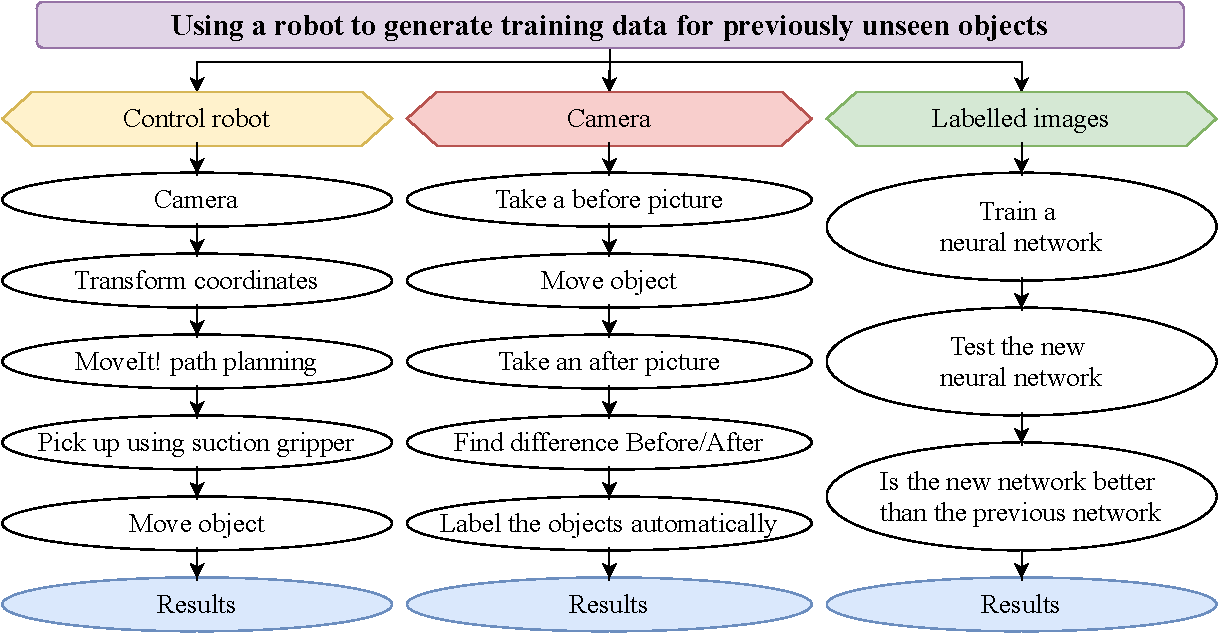
\includegraphics[width=1\textwidth]{graphics/meis.pdf}
    \caption{An flowchart that shows how the project is divided}
    \label{fig:project}
\end{figure}


\section{Background}
% \ifdraft{Provide background about the subject matter (e.g. How was morse code
% developed?  How is it used today?). 
% This is a place where there are usually many citations.
% It is suspicious when there is not.
% Include the purpose of the different equipment and your design intent. 
% Include references to relevant scientific/technical work and books.
% What other examples of similar designs exist?
% How is your approach distinctive?

% If you have specifications or related standards, these must be
% described and cited also.  As an example, you might cite the specific
% RoboSub competition website (and documents) if working on the lighting system for an AUV%\cite{guls2016auvlight}

% %% Glossary is broken, do not use --foley
% % \gls{auv}\footnote{Autonomous Undersea Vehicle}.

% % Notice that there is now information on the AUV in the Index and Acronyms.
% % It isn't in the \gls{glossary} because we didn't put it there.
% % \index{AUV}
% }{}

\subsection{Bin picking}\label{sec:binpicking}
Since the development of the first industrial robot, the automation of handling tasks has been an important scientific topic. In this context, one of the examples is the so-called “bin picking” problem\cite{buchholz_bin-picking_2016}. 
For humans, it is an easy task to pick up objects in a box, but it can be a very complex task for robots. 
Bin picking contains several subsections, including, scene analysis, object recognition, object localization, grasp planning, and path planning. 
Besides, robots must be able to grasp objects in an infinite number of directions and reach deep into the corners of the bin, at the same time avoiding collisions \cite{truebenbach_is_2019}.

Bin picking can be divided into three categories: \textit{Structured bin picking}, \textit{Semi-structured Bin picking}, and \textit{Random Bin picking}. The main difference between those categories is the difficulty level. In \textit{Structured bin picking} objects are placed in an organized pattern so that they can be identified and picked up effortlessly. In \textit{Semi-structured Bin picking} objects are placed with some organization to make picking easier. Finally, in the \textit{Random Bin picking}, objects have completely random positions, multiple directions, and can also overlap each other \cite{noauthor_future_nodate}.

For the bin picking to be fully automated it requires many technologies to work together. Including, a 3D model of the object, the bin, the robot end effector, the placement. Also, a model of ways to pick up the objects with the end effector and deposit it at the placement target. A 3D sensor to map the bin, image analysis software to locate each object and obstacle in the bin, path planning software to avoid collisions. Finally, a robot control software to maneuver the robot \cite{truebenbach_is_2019}.


In the setup and programming, there does the teaching takes place e.g. how to pick up an object, where to put it down, obstacles to avoid, etc. Path planning is another important task for system reliability, but this task is outside the scope of this thesis. 
To plan a unique, collision-free path for each object in the bin to the placement target. Path planning is the main determinant of system reliability because if it is not done well enough the objects can be dropped, left out in the bin, or missed targets and there can be collisions \cite{zeng_robotic_2019}.




\subsection{Computer Vision}
%% Úr bók A Guided Tour of computer vision.
The automatic deduction of the structure and properties of a possible complex three-dimensional universe from either a single or several two-dimensional representations of the world is known as computer vision or image comprehension\cite{nalwa_what_1994}. 
Computer vision (CV) is used to deduce the structure and properties of the three-dimensional universe, which include not only geometric properties but also material properties and the lighting of the world. 
The lightness or darkness of surfaces, their colors, textures, and material compositions are examples of geometric properties. Whereas the forms, sizes, and locations of objects are examples of material properties\cite{szeliski_computer_2010}. % úr bók af bókasafni

CV is an artificial intelligence-assisted paradigm that uses cameras, videos, and deep-learning methods to detect the digital world. Parallel to this, CV researchers have been working on mathematical methods for restoring the three-dimensional form and appearance of objects in images\cite{guo_lossy_2018}. 
Designers now have effective methods for constructing a partial 3D model of an area from thousands of partially overlapping images. Designers can construct accurate dense 3D surface models using stereo matching if they have a wide enough collection of views of a particular object or facade\cite{liu_detection_2020}. 
It also entails the development of specific technologies like image recognition, visual recognition, and facial recognition. Mostly, CV is used to achieve a high-level understanding of digital processing. The task of CV is to capture, examine, and recognize digital objects and extracts in higher dimensions\cite{manogaran_wearable_2019}.
%Designers can also follow a person's movements with a complex background. 

% \textbf{It is also possible to use a combination of face, clothes, and hair identification and recognition, to find and name all of the people in an image with moderate success. }\fxfatal{ÞARF AÐ LAGA Reference to old}

% \begin{figure}[ht]
%     \centering
%     % include first image
%     \subfloat[]{\includegraphics[width=0.2\textwidth]{graphics/compa.PNG}}
%     \hfill
%     %\subfloat[]{\includegraphics[width=0.2    \textwidth]{graphics/compb.PNG}}
%     %\hfill
%     \subfloat[]{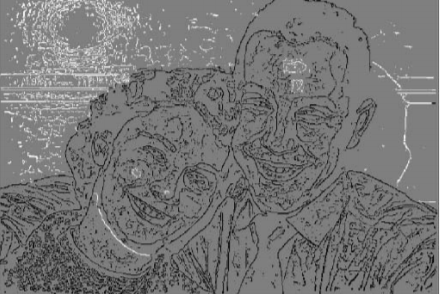
\includegraphics[width=0.2\textwidth]{graphics/compc.PNG}}
%     \hfill
%     \subfloat[]{\includegraphics[width=0.2\textwidth]{graphics/compd.PNG}}
%     \caption{fddsa}
%     \label{figure: computervision}
% \end{figure}
\begin{figure}[ht]
    \centering
    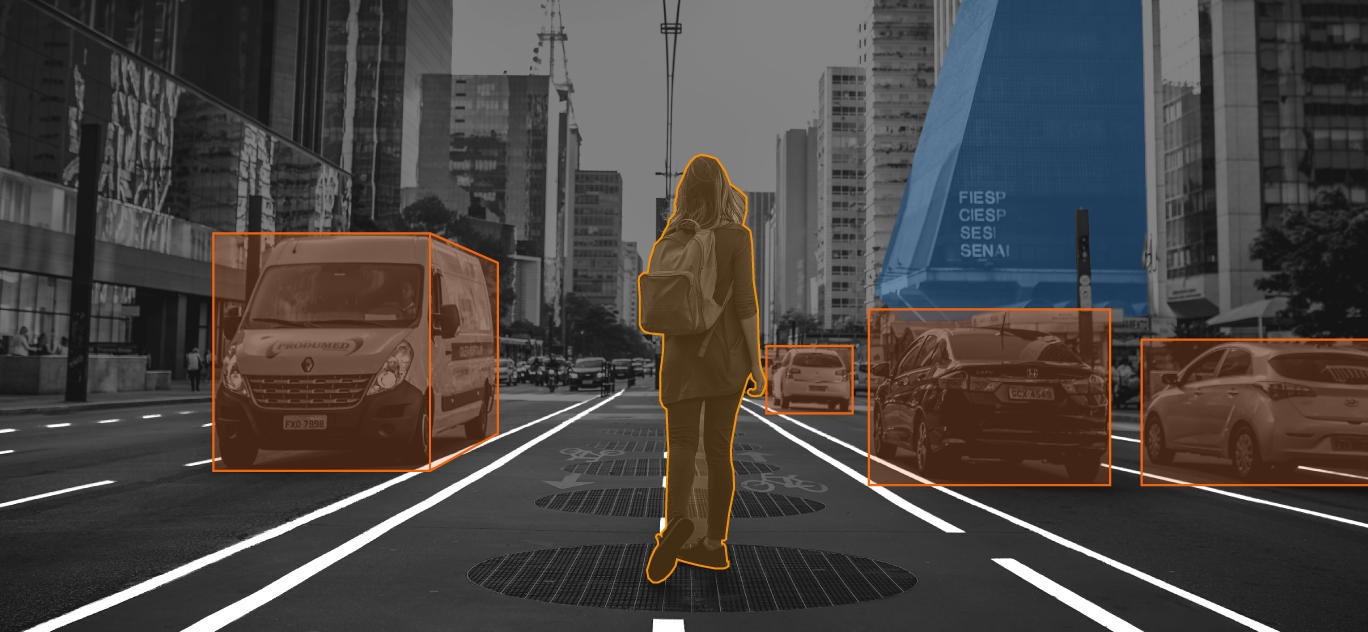
\includegraphics[width=0.85\textwidth]{graphics/mask.png}
    \caption{Computer vision plays a huge role in artificial intelligence, this is a example of a image that has been masked before using as a training data in a neural network  \cite{ambalina_5_2020}}
    \label{fig:mask}
\end{figure}

Computer vision is a branch of computer science that aims to replicate aspects of the complexity of the human vision system, allowing computers to recognize and process objects in images and videos in the same way that human eyes do. Pattern recognition is at the heart of computer vision. One method of teaching a computer to understand visual data is to feed it thousands of images, if not millions, of labeled images. Then subject the images to various software techniques, or algorithms, that allow the computer to search for patterns in all the elements that relate to those labels \cite{mihajlovic_everything_2019}.

The poster child of artificial intelligence is computer vision technology. Because of the resources and opportunities that technology can bring, this is the business area that attracts the most media coverage. From self-driving cars and drones to cancer detection and augmented reality, technologies that were once only seen in science fiction are now more accessible and available to us \cite{ambalina_5_2020}.




\subsubsection*{Edge detection} 
An image edge is a contour along which the image intensity suddenly changes and an image-intensity edge may or may not correlate to a physical edge of an object. The Canny operator\cite{nalwa_edge_1993} is a common edge detection operator that uses Gaussian smoothing. When the gradient magnitude exceeds a certain threshold, it detects edges at the zero-crossing of the smoothed image's second directional derivative in the direction of the gradient. Canny's filter is derived by optimizing a particular performance index that favors true positives, true negatives, and accurate localization of detected edges.

\begin{figure}[ht]
    \centering
    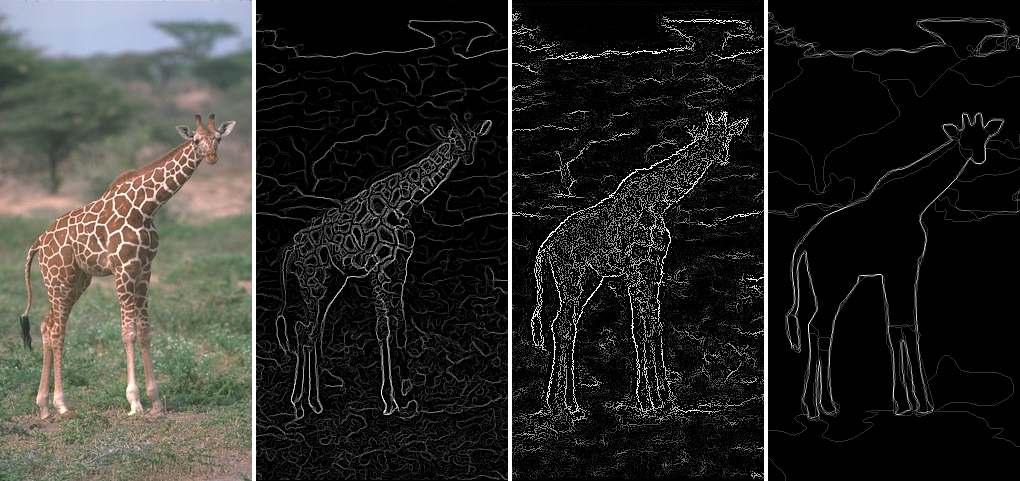
\includegraphics[width=0.8\textwidth]{graphics/canny.png}
    \caption{Example of edge detection \cite{nalwa_edge_1993}}
    \label{fig:edgedetection}
\end{figure}
%\subsubsection*{Point cloud}

%% Skoða hough transform...



% All edgel detectors seek to verify the existence of short linear edge segments that are postulated across image windows that have the same shape and size as the operator kernel. 


% skoða hough transform.
%% https://scholar.google.is/scholar?q=hough+transform+edge+detection&hl=en&as_sdt=0&as_vis=1&oi=scholart

%       \ifdraft{Hægt að sjá linka i links.tex}

%%%%%%%%%%%%%%%%%%%%%%%%%%%%%%%%%%%%%%%%%%%%%%%%%%%%%%%%%%%%%%%%%%
\subsubsection*{Convolutional neural network}
%\textbf{ÞARF AÐ BREYTA ÞESSUM kafla skoða comment fra martin}
% I think this chapter needs some more information about CNN:s (along with the appropriate references). What are they? How do they work? What does a typical CNN architecture look like? How many layers? What are the operations? What is the input? What is the output? etc.\textbf{It would be good to say something about why that is e.g. when using other machine learning methods like e.g. random forest you need to construct features}. 
In deep learning, a Convolutional Neural Network (ConvNet/CNN) is a class of deep neural networks that is most applied to images, assign importance to various objects in the image, and differentiating one from the other. In CNN the pre-processing is much lower as compared to other classification algorithms. While the filters for primitive methods are man-made, ConvNets can learn these filters/filters with adequate training. CNN's advantages include that it can successfully capture the spatial and temporal dependencies in an image through the application of relevant filters. CNN was inspired by the organization of the visual cortex and the connectivity pattern of neurons in the human brain\cite{saha_comprehensive_2018}. 

To detect objects, recognize faces, etc, CNN uses image recognition and classification. They consist of neurons with learning weights and preconditions. Each particular neuron received numerous inputs, then received a weighted sum, passed by an activation function, and replied with an output. CNN's are primarily used in the classification, grouping, and recognition of objects by similarities. Many CNN algorithms can recognize the faces, road signs, animals, etc\cite{bansari_introduction_2019}.

\begin{figure}[h]
    \centering
    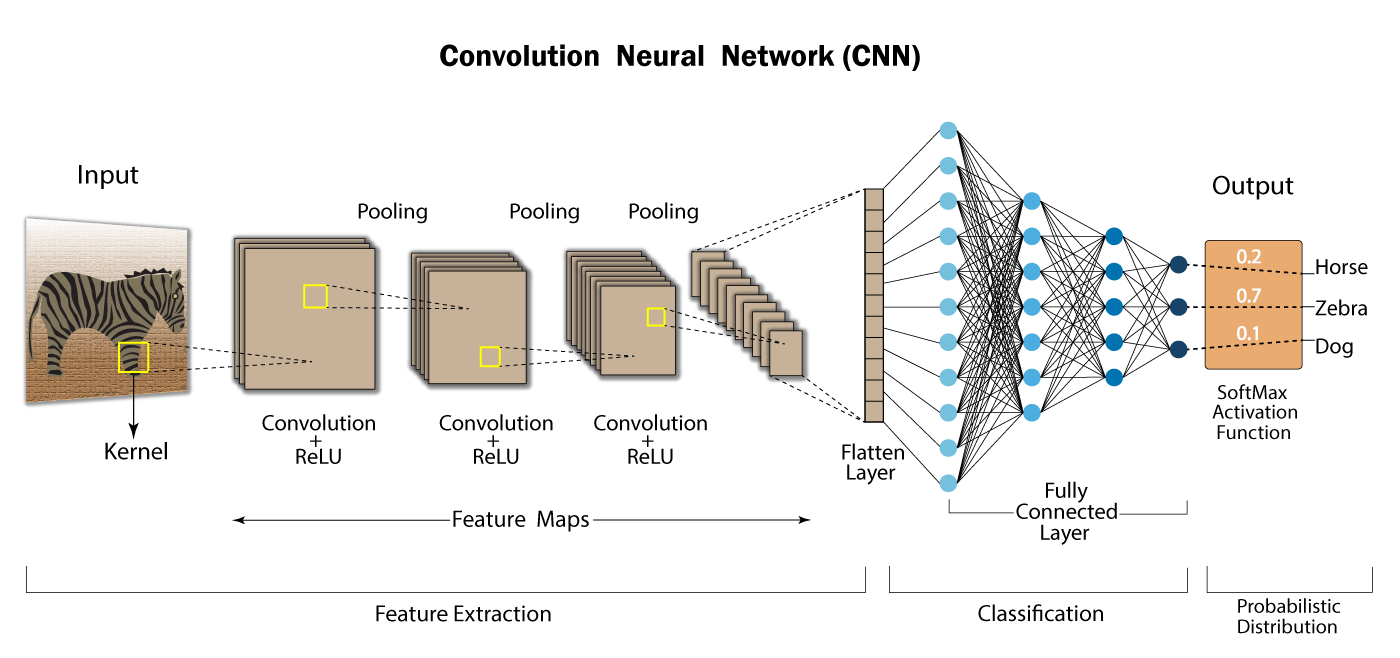
\includegraphics[width=1\textwidth]{graphics/methods/cnn.png}
    \caption{An example of how a CNN works\cite{swapna_convolutional_2020}}
    \label{fig:cnn}
\end{figure}

The CNN structure generally consists of two layers One feature is the extraction layer, each neuron input is connected to previous layers' local receptive fields, and the local feature is extracted. 
The position relation between this and other features will also be determined when the local features are extracted. The second is a map layer, and each network computer layer consists of a multi-function map. 
CNN is used primarily to indicate displacement, zoom, and other distorting graphical invariance forms. 
Since the CNN functional detection layer learns by training data, explicit extraction of functionality is avoided, and training data are taught when using CNN implicitly\cite{liu_implementation_2015}. An example of how a CNN works and looks like in \textit{Figure \ref{fig:cnn}}




\subsubsection*{Object detection}
Object detection is an important task for computer vision that deals with the detection of instances of certain class objects in digital images (e.g. people, animals, or cars) an example is shown in \textit{Figure \ref{fig:mask}}. Object detection aims to develop models and techniques for computer vision that offer one of the most basic information necessary for computer vision applications\cite{zou_object_2019}. \textit{Where are these objects?}

\begin{figure}[h]
    \centering
    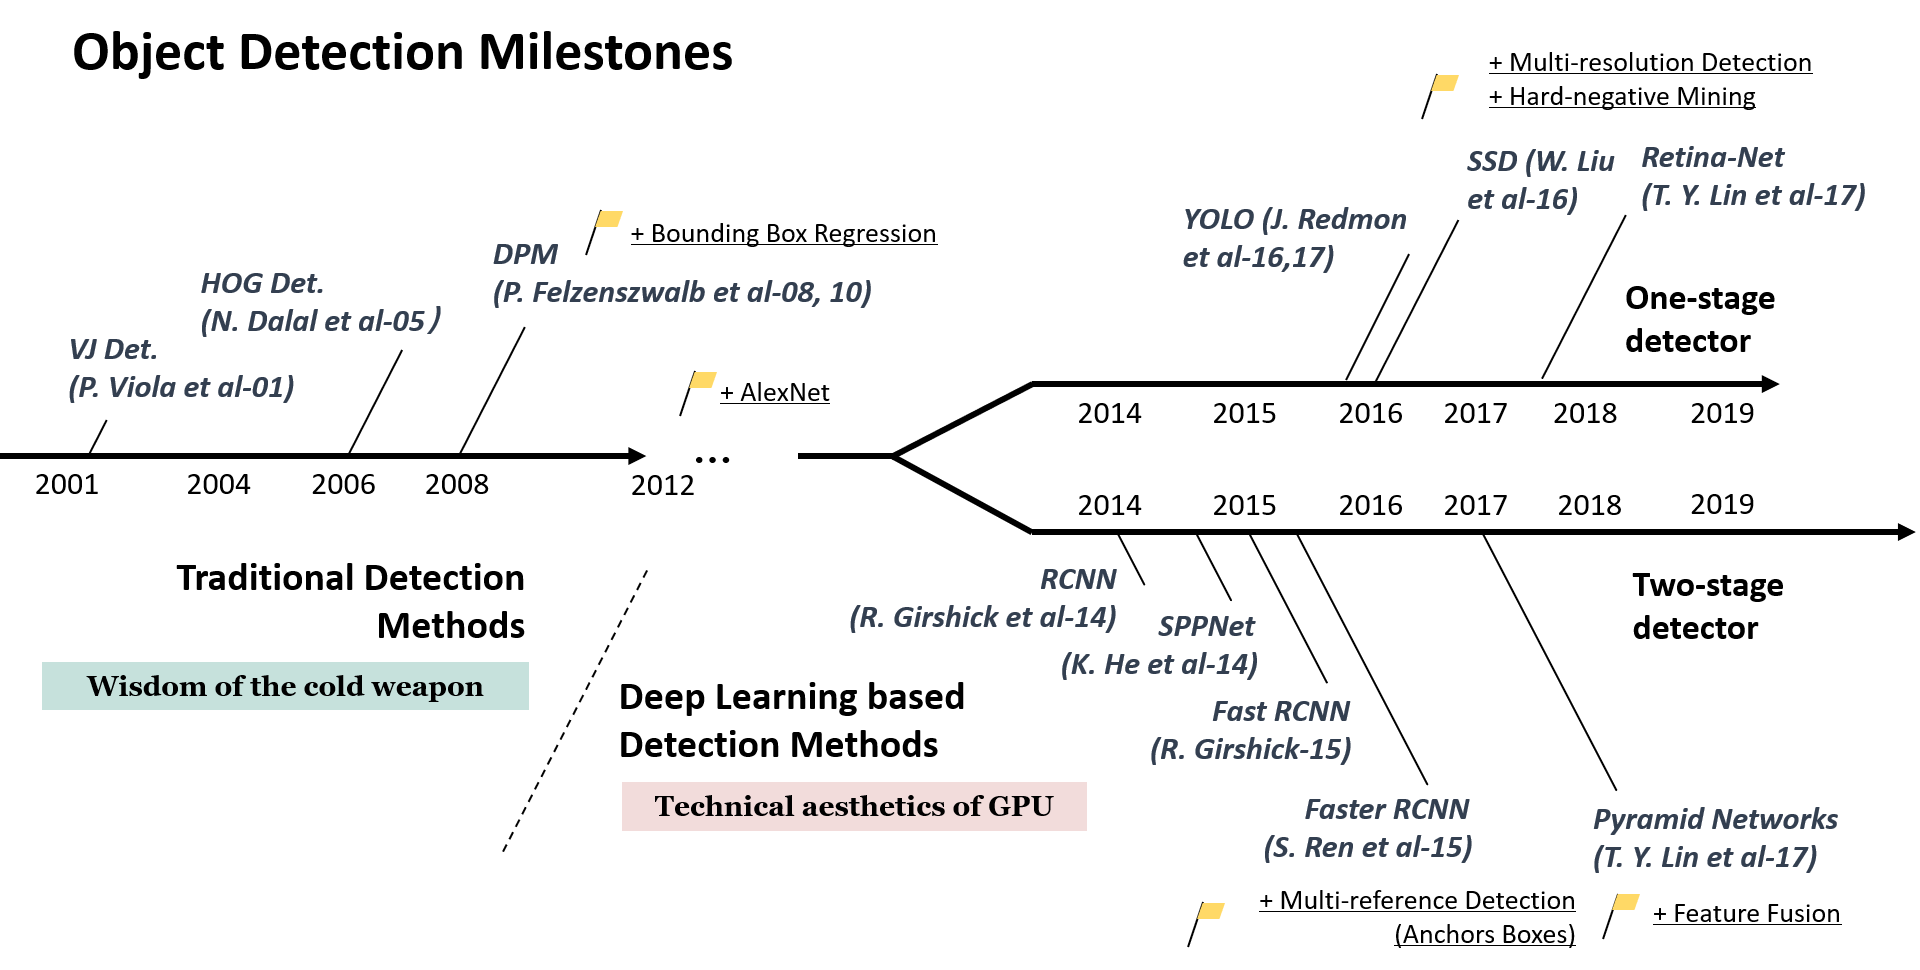
\includegraphics[width=0.9\textwidth]{graphics/objectdetection.png}
    \caption{Milestones in object detection \cite{zou_object_2019}}
    \label{fig:milestones}
\end{figure}
It has been widely accepted over the past two decades that the progress of object detection has usually been carried through two periods: the "traditional object detection (pre-2014)" and the "deep learning detection period" (post-2014). Milestones in object detections can be seen in \textit{Figure \ref{fig:milestones}}, in that figure it can be that there are many algorithms used for object detection. Some of the most commonly ones are \textit{Region-based Convolutional Neural Networks(R-CNN)}\cite{girshick_region-based_2016}, \textit{Fast R-CNN}\cite{girshick_fast_2015}, \textit{Faster R-CNN}\cite{ren_faster_2016}, \textit{Histogram of Oriented Gradients(HOG)}\cite{dalal_histograms_2005}, and \textit{You only look once(YOLO)}\cite{redmon_you_2016}.
%ÓKLÁRAÐ
\clearpage

% \subsection{Incremental Learning}
% \ifdraft{Hægt að sjá linka i links.tex}

%%%%%%%%%%%%%%%%%%%%%%%%%%%%%%%%%%%%%%%%%%%%%%%%%%%%%%%%%%%%%%%
\subsection{Robots}
Robots are getting smarter day by day and people wonder how much we can trust them in the industry. Collaborative Robots (Cobots) are more modern advances in which robots operate alongside humans rather than replacing them \cite{pickett_dont_2018}. 

Cobots assist operators by growing their capacities in terms of effort, enabling them to handle parts that are hot, heavy, bulky, or too fragile for precision handling. Besides, cobots are easier to program than industrial robots because they are capable of learning new jobs \cite{schmidbauer_teaching_2020}. A factory worker can easily re-program cobot, simply by moving his arm along the desired track. From there the cobot would learn the new movement and be able to replicate it on his own. Industrial robots can not be reprogrammed as easily and require the engineer to write a new code for any improvements in the process to be implemented.

Industrial automation is capable of achieving high productivity and repeatability in mass manufacturing. However, there is a lack of flexibility to overcome the uncertainties of workspaces arising from mass customization \cite{accorsi_application_2019}. Although humans can cope with such uncertainties and variability in such circumstances, their physical capacities are constrained in terms of repeatability, physical power, endurance, speed, etc. These constraints also lead to decreased performance and productivity. Therefore, a combination of automation and versatility is required to meet these overall manufacturing objectives through mass customization \cite{zaatari_cobot_2019}.   

\subsubsection*{Mathematical Robot Modeling:}
A mathematical representation must be built to generate trajectories and tasks for robots. This includes a model of the robot's geometry, mechanics, and electrical components. The mathematical model is developed to create a quantitative relationship between the sudden shift and the magnitude of the collision. The latter is represented by either an external impulsive force or an instantaneous change in the contact point's linear velocity. Second, as a result of the collision, large impulsive forces and constraint torques may develop within the system at each joint. These impulses can affect the system. A mathematical model is also established to create a quantitative relationship between the impulsive forces and torques of constraint and collision.  \cite{zheng_mathematical_1985}.

Robotic Manipulators are composed of two merged things, links, and joints that form a kinematic chain. In this context, links are the rigid sections that make up the mechanism and joints are the connection between two links. The kinematic manipulator chain is a combination of several cinematic pairs and the pair is a combination of two links connected by joint \cite{al-naimi_robotics_2018}.

\begin{figure}[h]
    \centering
    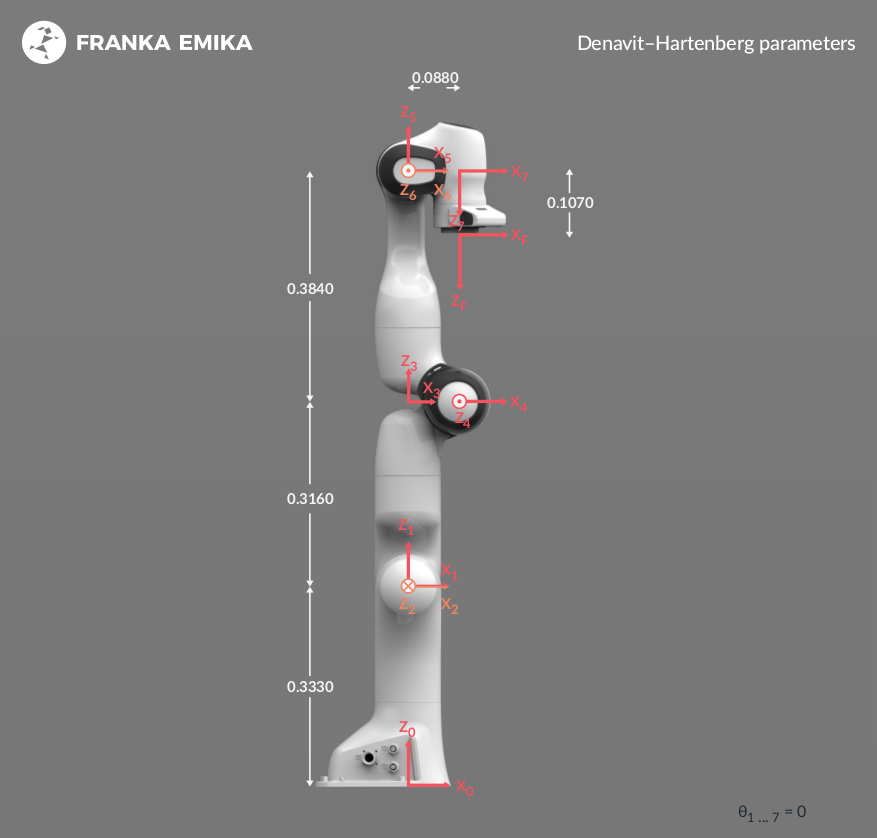
\includegraphics[width=0.7\textwidth]{graphics/pandakinematicchain.png}
    \caption{Panda’s kinematic chain \cite{noauthor_robot_2017}}
    \label{fig:pandachain}
\end{figure}

\subsubsection*{Coordinate frame Transformations}
 %\url{https://www.maplesoft.com/content/EngineeringFundamentals/13/MapleDocument_13/Position,%20Orientation%20and%20Coordinate%20Transformations.pdf}
A 3D space pose or link has a 6 degree degree (DOF), translation\textit{(x,y,z)} and rotation $R \in SO(3)$. Depending on the application, the rotations may be expressed in several formats. 
In robotics, rotation matrices, rotations of the axis, quaternions, and Euler angles are usually used to represent rotations.
A homogeneous matrix of transformation is a convenient way of bringing translations and rotations together to transform poses and coordinate frames\cite{cai_coordinate_2011}.

Three angles are the Euler angle of a rigid body which is introduced by Euler. Euler angles can describe the relative orientation between any two cartesian frames. After a rotation about the Z-axis, rotated Y-axis, and the rotated X-axis(or the so-called 3–2–1) the Euler angles are adopted and move the reference frame into the frame. These three Euler angles are also referred to as the yaw (or heading), pitch, and roll angles\cite{cai_coordinate_2011}.

The three matrices of relative rotation are given by:
\begin{equation}
    R_{int1/nv} = R_{z}(\psi) = \begin{bmatrix}
cos(\psi)  & sin(\psi) & 0\\ 
-sin(\psi) & cos(\psi) & 0 \\ 
0 & 0 & 1
\end{bmatrix},
\end{equation}\label{eq:rz}

\begin{equation}
    R_{int2/int1} = = R_{y}(\theta) =  \begin{bmatrix}
cos(\theta)  & 0 & -sin(\theta)\\ 
0 & 1 & 0 \\ 
sin(\theta) & 0 & cos(\theta)
\end{bmatrix},
\end{equation}\label{eq:ry}
and 
\begin{equation}
    R_{b/int2} = R_{x}(\phi) =\begin{bmatrix}
1  & 0 & 0\\ 
0 & cos(\phi) & sin(\phi) \\ 
0 & -sin(\phi) & cos(\phi)
\end{bmatrix}.
\end{equation}\label{eq:rx}


For each angle axis, the Equations (\ref{eq:rz}), (\ref{eq:ry}) and (\ref{eq:rx})  show rotation matrices that can then be used for rotating around a fixed body or axis. An intrinsic rotation is a rotation on a body frame, whereas the external rotation is defined as an elemental rotation around a defined coordinate axis.
\begin{equation}
    R_{z(\psi)y(\theta)x(\phi)} = R_{z(\psi)} R_{z(\theta)}R_{x(\phi)}
\end{equation}
%Skoða
%\url{https://sci-hub.se/10.1007/978-0-85729-635-1_2} ... Þarf að skrifa úr þessu 


\subsection{Robot Operating System (ROS)}
Robot Operating System (ROS) is an open-source flexible framework for developing robot applications. It is a set of software, libraries, and conventions aimed at making the challenge of developing dynamic and robust robot actions over a wide range of robotic platforms easier. ROS is not a conventional operating system in the context of process control and scheduling \cite{quigley_ros_2009}. ROS offers package processing, message services between devices, and a variety of libraries. ROS supports a variety of programming languages, including C++, Python, and Javascript. ROS has over 3000 packages available, including robot drivers, computer vision libraries, navigation applications, and many more.
% \\
% \\ Það á eftir að skrifa þessa kafla hér :::::
% \textbf{Collision Detection:}
% \newline
% \textbf{Motion Planning:}
% \newline

\begin{figure}[h]%left, bottom, right and top
    \centering
    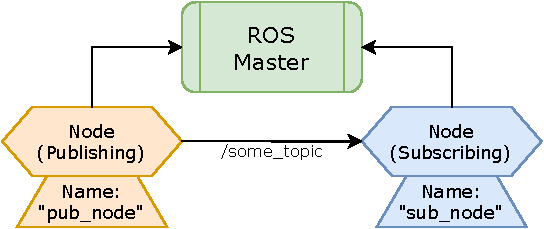
\includegraphics[width=0.8\textwidth]{graphics/rosmaster.pdf}
    \caption{This figure shows a basic ROS setup. The ROS master manages and establishes node connectivity. The correspondence is made by the subject /some\_topic in this example.}
    \label{fig:rosmaster}
\end{figure}

In a running ROS system, the \textbf{ROS Master} offers name and registration services to the other ROS nodes. It follows the topics and resources of the publishers and subscribers. The job of the master is to allow the location of individual ROS nodes. After these nodes are placed, they interact peer-to-peer\cite{wu_master_2018}. An example of an ROS master can been seen in \textit{Figure \ref{fig:rosmaster}}.


\textbf{ROS nodes} are modules of the program which execute an operation. 
The nodes are autonomous and can be programmed in a programming language while also communicating in a different language with other nodes\cite{meier_understanding_2019}. An example of an ROS nodes can been seen in \textit{Figure \ref{fig:rosmaster}}.


The \textbf{ROS topics} are buses that exchange messages between nodes, implemented as named shared memory locations. Anonymous subjects have semantics publish/subscribe that decouple data output from consumption. Nodes are not generally aware of who they talk to. Instead, nodes interested in data subscribe to the subject concerned, and nodes that generate data publish to a specific topic. Many publishers and subscribers may participate in an issue\cite{foote_topics_2019}. An example of an ROS topic can been seen in \textit{Figure \ref{fig:rosmaster}}.

A set of software packages integrated with the ROS and designed specifically to be aware of their surroundings and avoid collisions with humans and other obstacles is called \textbf{MoveIt!}. MoveIt! package implements solutions to the path planning problems that were mentioned in \textit{Section \ref{sec:binpicking}}. 
By using data fused from 3-D and other sensors, MoveIt! will allow robots to build up a representation of their environment. Also, generate motion plans that effectively and safely move the robot around in the environment, and execute the motion plans while constantly monitoring the environment for changes. 
%In other words, MoveIt! is an evolution arm navigation packages which were designed for motion planning and to create trajectories for simple paths with a single goal pose. 
MoveIt! provides a framework e.g., manipulation, kinematics, and motion planning. To calculate inverse and forward kinematics for path planning, and MoveIt packages use Unified Robot Description Format(URDF). Configurations can then be created using the MoveIt set up assistant \cite{chitta_moveit_2012}.

%------------------------------------
\section{Evaluation metrics}
\subsection{Intersection over union}
Intersection over Union (IoU) is known to be a good metric for overlapping two bounding boxes or masks and is used to measure object detector accuracy on a certain dataset. If the estimate is correct, then IoU = 1. The lower the IoU, the worse is the results \cite{sheremet_intersection_2020}.

\begin{figure}[h]
    \centering
    % include first image
    \subfloat[An example of a stop sign being detected in a picture. The prediction bounding box is red and the bounding box of the ground-truth is green. ]{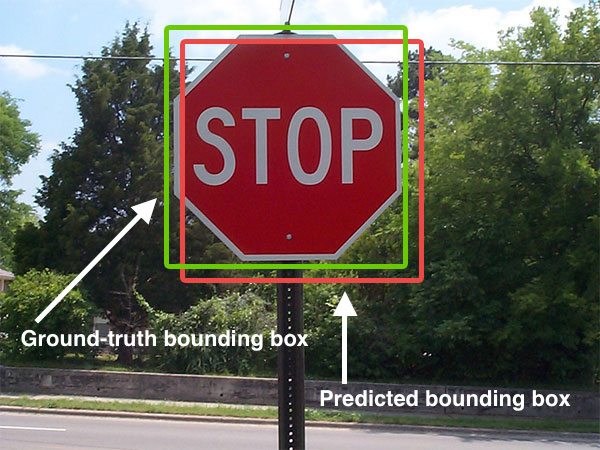
\includegraphics[width=0.48\textwidth]{graphics/iou_stop_sign.jpg}}
    \hfill
    \subfloat[The Intersection of Union are as simple as dividing the overlap zone between boundaries by the union area]{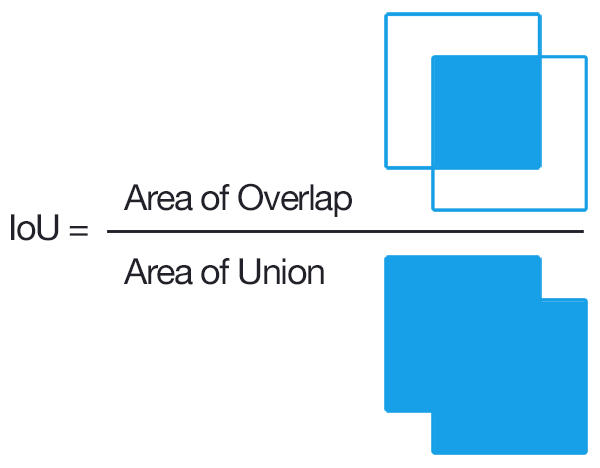
\includegraphics[width=0.48\textwidth]{graphics/iou_equation.png}\label{figure: ioueq}}
    \caption{Intersection over Union for object detection \cite{rosebrock_intersection_2016}}
    \label{figure: iou}
\end{figure}

\begin{equation}
    IoU = \frac{Area\ of\ Overlap}{Area\ of\ Union} \label{eq: ioueq}
\end{equation}
\vspace{0.5cm}

Intersection over Union is simply a ratio between the area of overlap and area of the union when looking at \textit{Equation \ref{eq: ioueq}}.
In the numerator, the area of overlap is calculated between the predicted bounding box and the bounding box.
The denominator is the area of union or, rather, the area covered by both the foreseen boundary and the bottom-wheel boundary\cite{uavs_comparing_2019}.
%\vspace{1cm}
\subsection{Recall, Precision, and F1}
When tests of the performance on the retrieval systems were first developed, an empirical tendency was noticed for recall (completeness) and accuracy (cleanliness of retrieval), both of which appeared to be inversely connected\cite{buckland_relationship_1994}. \textit{Figure \ref{fig:precisionrecall}} explains the precision and recall.



\begin{itemize}
    \item True Positive (TP): The actual positive class is predicted positive.
    \item True Negative (TN): The actual negative class is predicted negative.
    \item False Positive (FP): The actual class is negative but the predicted class is Positive
    \item False Negative (FN): The actual class is positive but the predicted class is negative.
\end{itemize}

\begin{figure}[h]
    \centering
    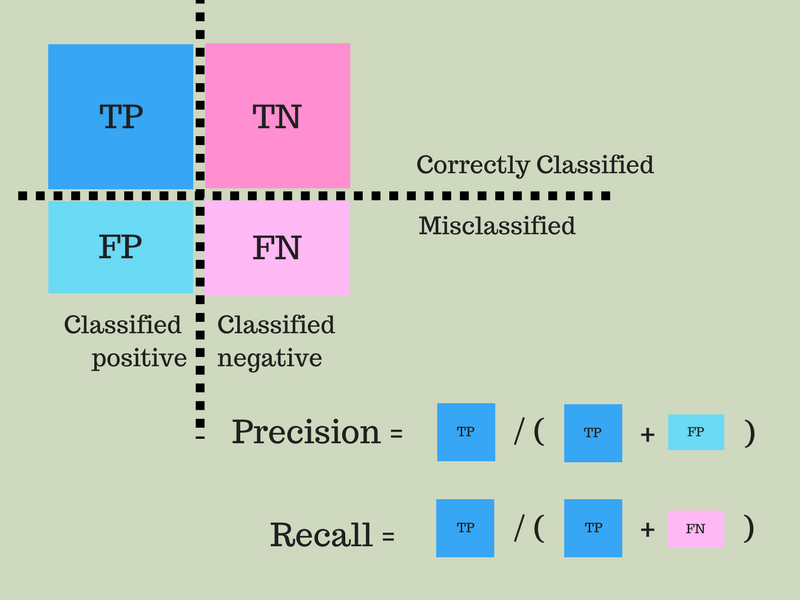
\includegraphics[width=0.8\textwidth]{graphics/Precisionrecall.png}
    \caption{Precision and recall explained \cite{mittapally_whats_2019}}
    \label{fig:precisionrecall}
\end{figure}



Precision is the ratio between the True Positives and all the Positives. In this project, the precision was measured by the number of bottles that were correctly identified out of all the bottles in the bin. It can bee seen in \textit{Equation \ref{eq:precision}}. Precision shows a measure of relevant data points\cite{shung_accuracy_2018}.
\begin{equation}
    Precision = \frac{True\ Positive(TP)}{True\ Positive(TP)+False \ Positive(FP)}
    \label{eq:precision}
\end{equation}


The recall is the measurement of the model that identifies true positives properly. Recall calculates the number of the correct detections divided by the number of actual detections\cite{shung_accuracy_2018}. Recall quantifies the number of positive class predictions made out of all positive examples in the dataset. An example of how recall is calculated can be seen in \textit{Equation \ref{eq:recall}}.
\begin{equation}
    Recall = \frac{True\ Positive(TP)}{True\ Positive(TP)+False \ Negative(FN)}
    \label{eq:recall}
\end{equation}

The F-score is a measure of the precision of a model on a dataset. This evaluation is done to evaluate binary classification systems, classifying examples into positive or negative classification systems. 
The F-score combined the precision and recall of the model and is described as the harmonic mean to the precision and recall of the model\cite{wood_f-score_2019}.
An example of how F-score is calculated can be seen in \textit{Equation \ref{eq:f1score}}.
\begin{equation}
    F- score = F_1 = 2 \cdot \frac{Precision \cdot Recall}{Precision + Recall}
    \label{eq:f1score}
\end{equation}


\section{Objectives}
The objective of this project was to answer the following research questions:
\begin{enumerate}[i.]
    \item Is it possible to generate new arrangements of objects using a robot manipulator?
    \item Is it possible to annotate objects automatically,  determining the extent of the objects in the images?
    \item Is it possible to improve the performance of a Convolutional Neural Network using automatically generated training data from a robot? %How will the accuracy of object detection be, using a deep neural network trained on the robot-generated data?
\end{enumerate}%%RUM: Introduction
\chapter{Methods}
This chapter describes the basic principles and strategies used to achieve the project objectives. 
\section{Software tools}
%\textit{Hér skrifa ég hvað ég notaði og hvernig og referenca í undirkafla í hvert skipti}

This chapter includes a brief overview of the software that was used in this project. 
ROS will be used to communicate between nodes and programs, the ROS distribution version will be the \textit{ROS Melodic Morenia}\cite{noauthor_melodic_nodate}. 
The main software programming language will be Python version 2.7 \cite{noauthor_python_nodate}, since that is a version that is supported by ROS Melodic.
In \textit{Figure \ref{fig:roswork}} shows the ROS setup in a flowchart that shows how the nodes communicate in this project.
\begin{figure}[h]
    \centering
    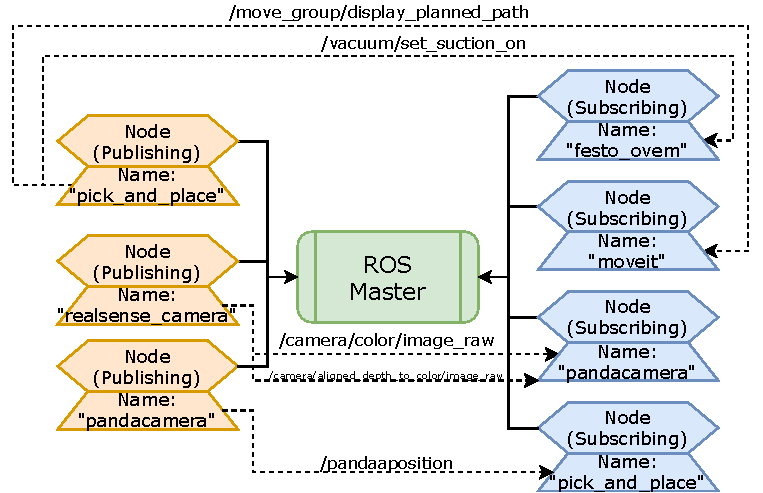
\includegraphics[width=0.7\textwidth]{graphics/ros.pdf}
    \caption{ROS setup}
    \label{fig:roswork}
\end{figure}

%The main hardware parts will be explained in several subsections: robot manipulator (\ref{subsec:robot}), robot end effector (\ref{subsec:robotend}) and a camera (\ref{subsec:camera}). 

\subsection{Data Annotation}
COCO Annotator is a web-based image annotation application that allows you to mark up images rapidly and conveniently to create training data for image localization and object detection. It has a variety of unique features, such as the ability to label an image segment, monitor object instances, label objects with disconnected visible sections, and store and export annotations in the well-known COCO format. An intuitive and customizable interface guides you through the annotation process, which includes a range of resources for constructing accurate datasets \cite{brooks_jsbrokscoco-annotator_2021}.
% \begin{figure}[h]
%     \centering
%     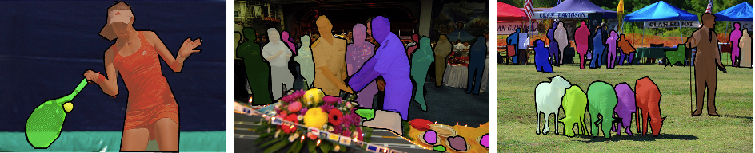
\includegraphics[width=1\textwidth]{graphics/coco.png}
%     \caption{An example of how images are annotated by hand}
%     \label{fig:coco}
% \end{figure}
% \linespread{0}

\subsection{Object detection}


You only look once (YOLO) is a real-time object detection system that is at the cutting edge of technology. 
It was first developed by Josep Redmon and is a convolutional neural network.
Object identification, classification, and localization are all performed in a single network pass with YOLO. 
As a result, it is more computationally efficient and robust than other networks that only perform one or two of these tasks at the same time. 
With the help of dimension clusters, YOLO predicts classes and bounding boxes (convolutional neural network). 
It's so computationally powerful that it can operate on a live image stream, which comes in handy when operating on a robot in real time \cite{redmon_yolov3_2018}.
\begin{figure} [ht]
    \centering
    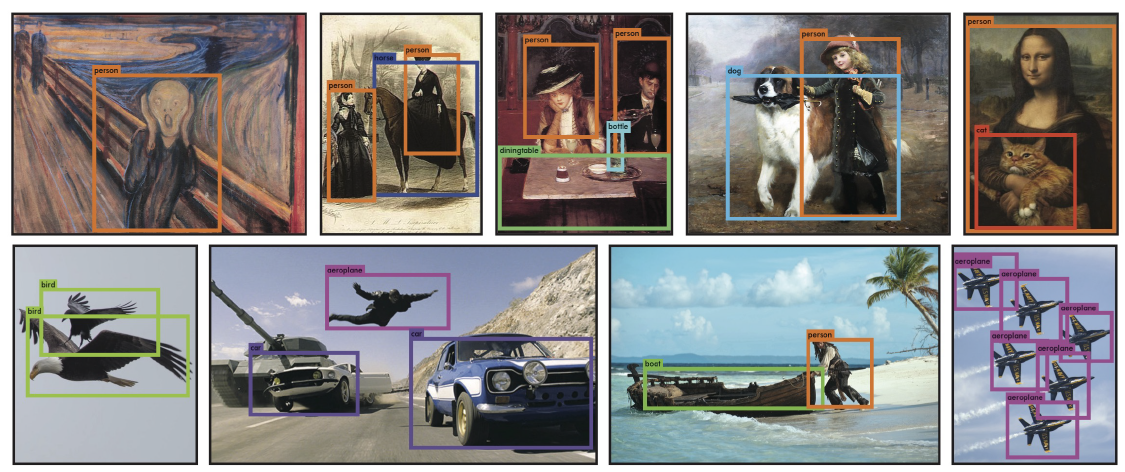
\includegraphics[width = 0.75 \textwidth]{graphics/yolo.PNG}
    \caption{You Only Look Once: Unified, Real-Time Object Detection \cite{redmon_you_2016}}
    \label{fig:yolo}
\end{figure}


In this project \textit{YOLOv4}\cite{bochkovskiy_yolov4_2020} algorithm was used to detect objects in the bin and mark a rectangle around them. 
YOLO algorithm was chosen since it is easy to use and the major advantage of YOLO is its excellent speed, it also understands the general representation of objects. YOLO algorithm outperforms other detection algorithms, including \textit{Deformable Parts Model(DPM)} and \textit{R-CNN}, when generalizing natural pictures from artworks to other fields\cite{zou_object_2019}.

%When the YOLO has found an object with high accuracy it sends to the robot coordinates of the center point, and then there is possible to get the depth from the camera.

% \begin{figure}[h]
%     \centering
%     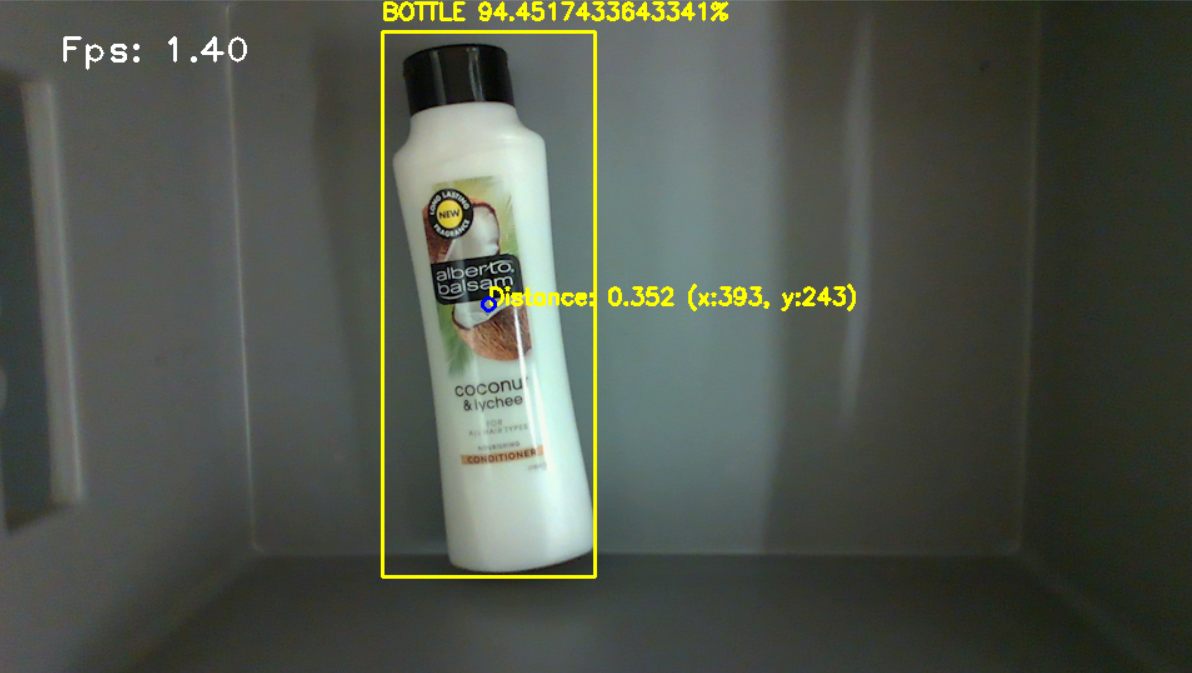
\includegraphics[width=0.4\textwidth]{graphics/detectandmeasure.PNG}
%     \caption{Here is an example of an YOLO detect application}
%     \label{fig:yolodetect}
% \end{figure}

\subsection{OpenCV}
OpenCV is a cross-platform library that allows one to build real-time computer vision applications. It is primarily concerned with image recognition, video capturing, and interpretation, with features such as face detection and object detection. OpenCV is a free and open-source library of programming functions primarily for real-time computer vision \cite{noauthor_opencv_nodate}.

One of OpenCV's aims is to provide an easy-to-use computer vision infrastructure that allows people to easily create fairly complex vision applications. Over 500 functions in the OpenCV library cover a wide range of vision applications, including factory product inspection, medical imaging, security, user interface, camera calibration, stereo vision, and robotics. Since computer vision and machine learning often go hand in hand, OpenCV includes a comprehensive, general-purpose Machine Learning library \cite{kaehler_what_2016}.

\begin{figure}[h]
    \centering
    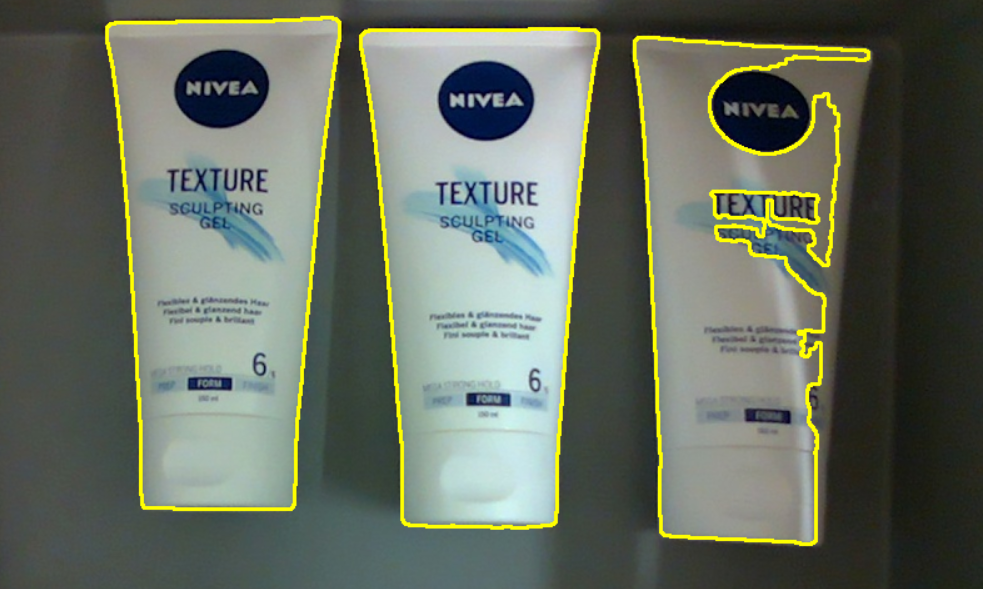
\includegraphics[width=0.65\textwidth]{graphics/contour.PNG}
    \caption{An example of how OpenCV can find contours}
    \label{fig:opencvcontour}
\end{figure}

OpenCV was used in this project to work on images from the camera, the main functions that were used in this project were \textit{structural simularity} to compute the difference between two images,  \textit{threshold} to threshold the difference image followed by finding contours to obtain the regions of the two input images that differ and then the \textit{findContours} function to find the contours, draw around the objects and measure the objects.
% breyta, say why I used each function and why opencv was used in that part....and so on44
% segja meira um hvern function t.d. structural simu og finna reference

\clearpage
\section{Hardware \label{sec:hardware}}
%\ifdraft{\textit{Hér skrifa ég hvað ég notaði og hvernig og referenca í undirkafla í hvert skipti (Má lesa yfir\\}}
This chapter includes a brief overview of the hardware that was used in this project. The main hardware parts will be explained in several subsections: robot manipulator \textit{(Sec:\ref{subsec:robot})}, robot end effector \textit{(Sec:\ref{subsec:robotend})} and a camera \textit{(Sec:\ref{subsec:camera})}. The setup can been seen in \textit{Figure \ref{fig:setupproject}}.

\begin{figure}[h]
    \centering
    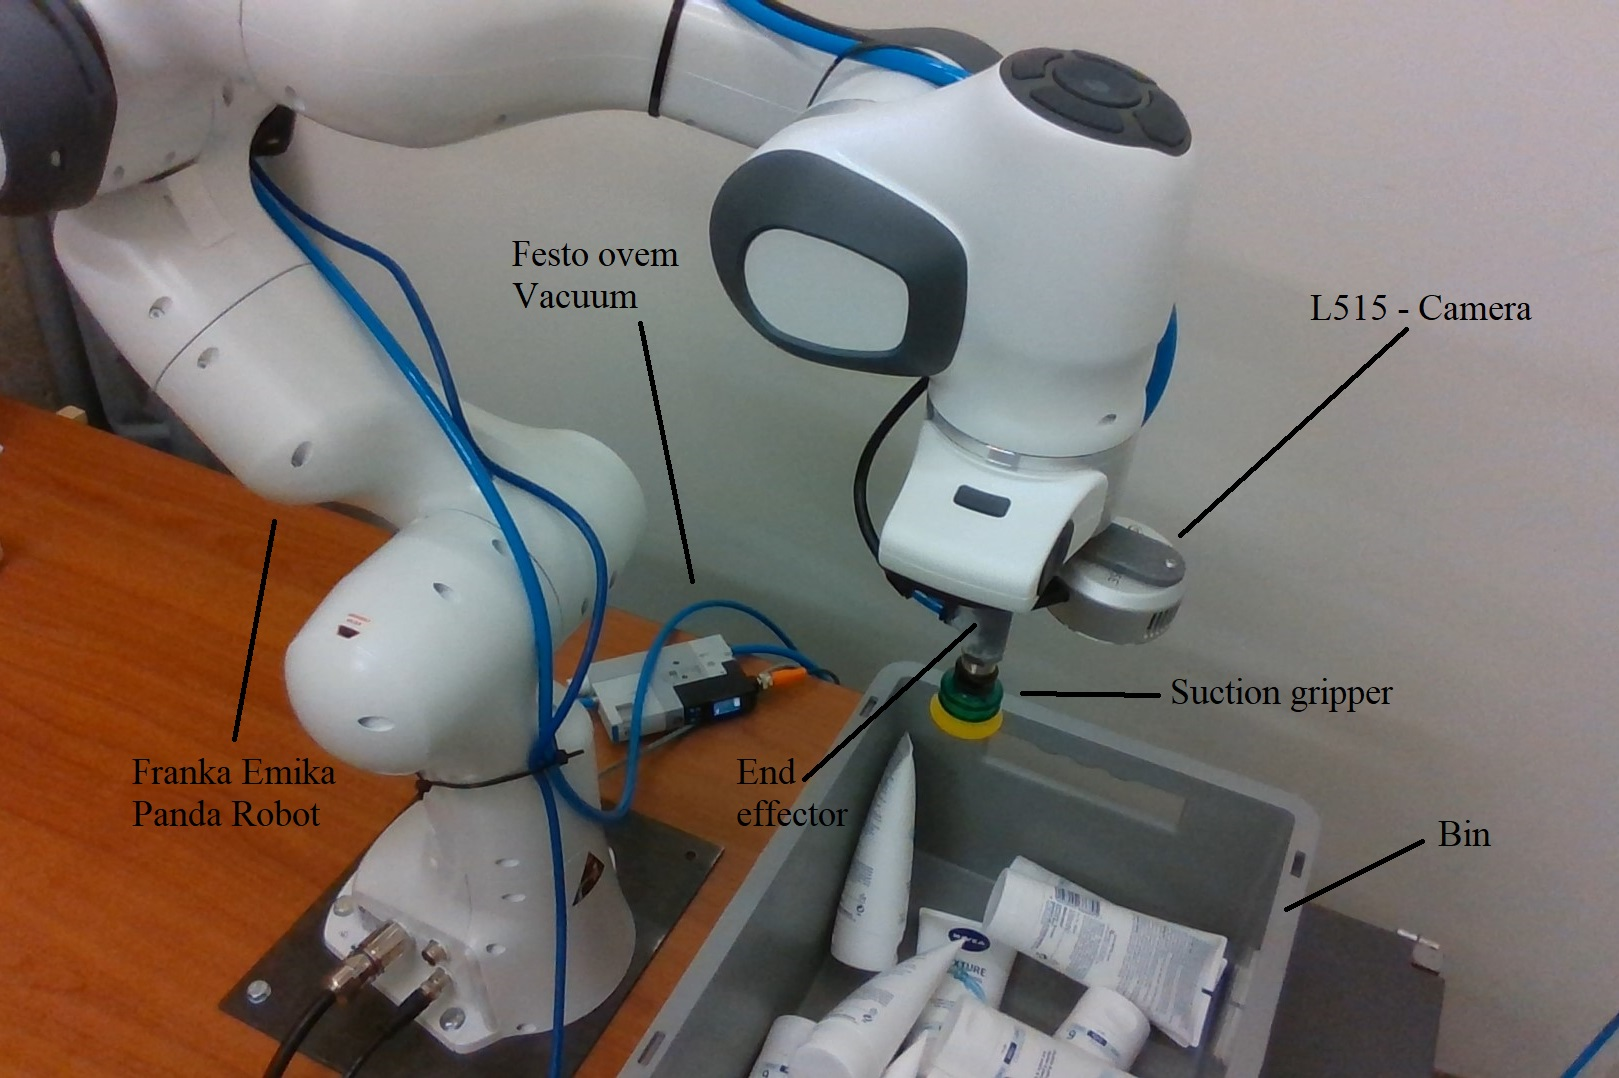
\includegraphics[width = 0.65\textwidth]{graphics/setup.jpg}
    \caption{The hardware setup for this project}
    \label{fig:setupproject}
\end{figure}
\linespread{0}
\subsection{PC cores}
\vspace{0.8cm}
\subsubsection*{Training neural networks}
The GPU for training neural networks will be the \textit{NVIDIA GeForce RTX 2080 Ti}\cite{noauthor_graphics_nodate}.
A GPU is nearly necessary to train neural networks. The GeForce RTX 2080 Ti is a budget-friendly option for the dense system configuration with a blower size. Titan RTX, Tesla V100, Titan V, GTX 1080 Ti, and Titan Xp provide the best price versus performance. Its performance at training neural networks is close to Tesla V100 speed, which is one of the world's most powerful GPU\cite{noauthor_deep_2018}. 

\subsubsection*{Computer to control the robot}
The computer that will be used in this project to control the robot is a \textit{Lenovo ThinkCentre M83 SFF Pro Desktop}\cite{noauthor_thinkcentre_nodate} computer, it was chosen since it has ROS and had already been used to program the Franka Emika robot. 

\clearpage

\subsection{Robot manipulator\label{subsec:robot}}
The Robot manipulator that was used in this project is a Franka Emika Panda robot, an research robot located at the RU(Reykjavik University) Robot Interaction Lab. Franka Emika Panda is a Cobot that has 7 working axes with torque sensors in all 7 axes \cite{gmbh_franka_nodate}. Panda includes the characteristics of a conventional stiff industrial robot with a repeatability of +/- 0.1 mm even at elevated velocities of up to 2 m/s with a negligible direction variance. This enables accurate, resilient, and quick manufacturing method execution. 
% \begin{figure}[h]
%     \centering
%     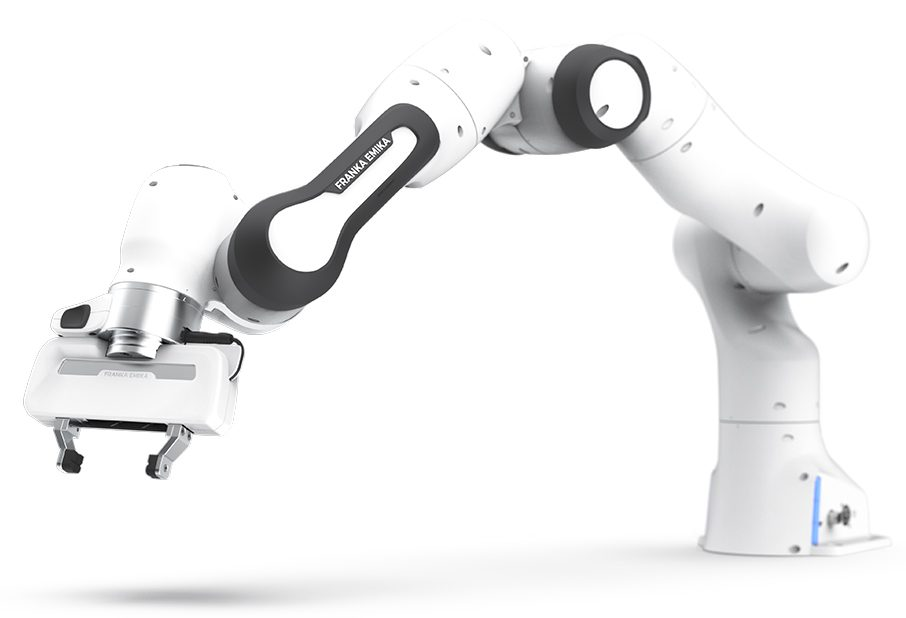
\includegraphics[width=0.8\textwidth]{graphics/frankapanda.jpg}
%     \caption{Franka Emika Panda}
%     \label{fig:frankaemika}
% \end{figure}
\begin{figure}[h]
    \centering
    % include first image
    \subfloat[Franka Emika Panda ]{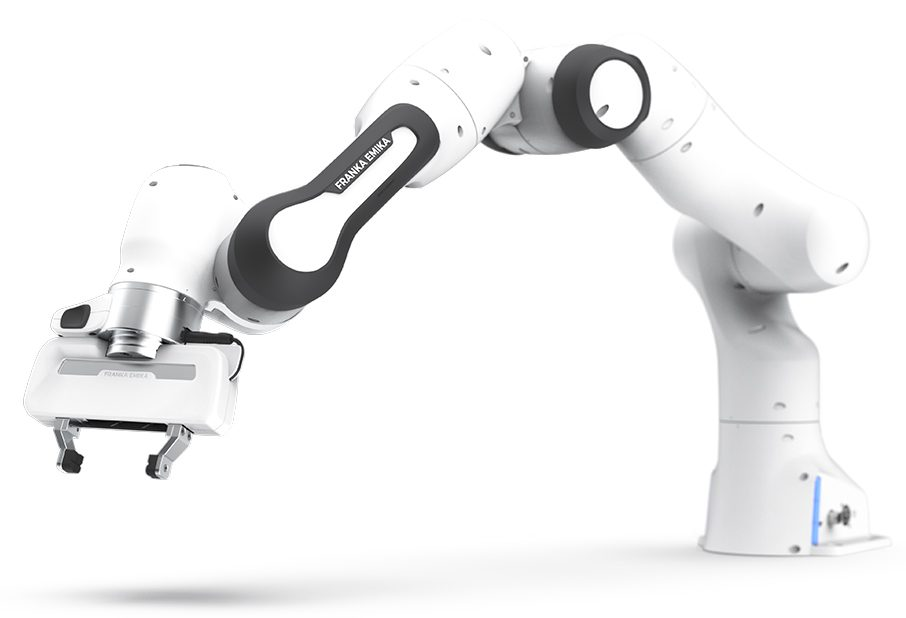
\includegraphics[width=0.6\textwidth]{graphics/frankapanda.jpg}}
    \hfill
    \subfloat[Franka Emika Panda setup]{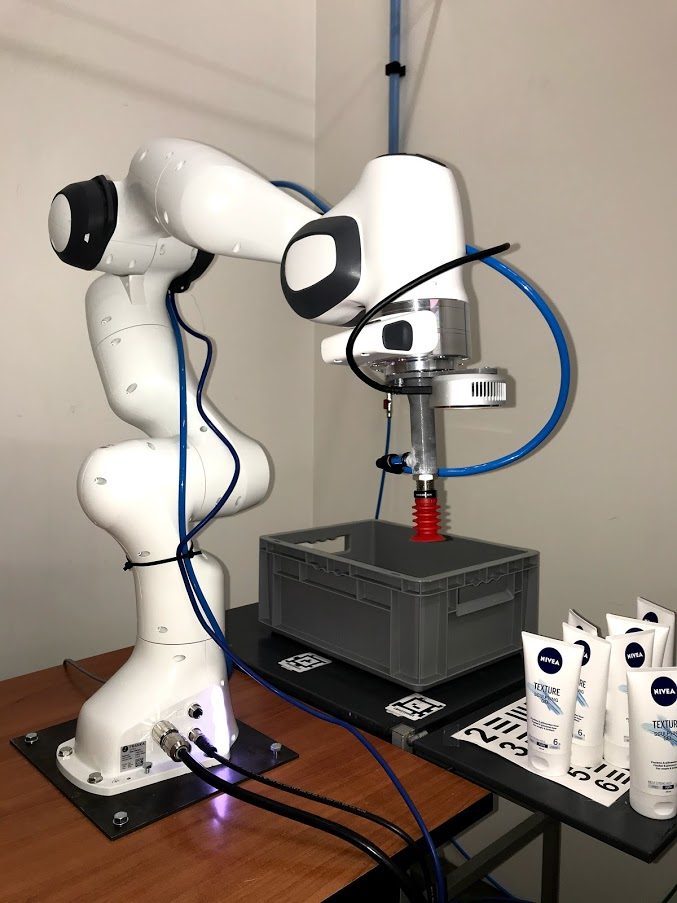
\includegraphics[width=0.35\textwidth]{graphics/pandarobot.jpg}}
    \caption{Robot manipulator}
    \label{figure: frankaemika}
\end{figure}
% Má eyða seinna\begin{itemize}
%     \item \url{https://www.franka.de/}
%     \item Franka Emika Panda in Gazebo with ROS and Docker \cite{wallkotter_franka_2020}
% \end{itemize}

\subsection{Robot end effector\label{subsec:robotend}}
A peripheral device that connects to a robot's wrist and allows it to communicate with its mission is known as an end effector. Grippers, process tools, and sensors are all examples of end effectors, which are mechanical or electromechanical \cite{wilson_relative_1996}. 

An suction gripper was designed and fabricated for use in the experiments, shown in \textit{Figure \ref{figure: endeffector}}.
It was designed in Autodesk Inventor \cite{noauthor_inventor_nodate} and 3D printed in TEVO Nereus 3D printer that Reykjavik University owns. At the end of the effector there is a suction cup connected to Festo Vacuum generator OVEM with an 8mm tube.
\begin{figure}[ht]
    \centering
    % include first image
    \subfloat[Inventor drawing ]{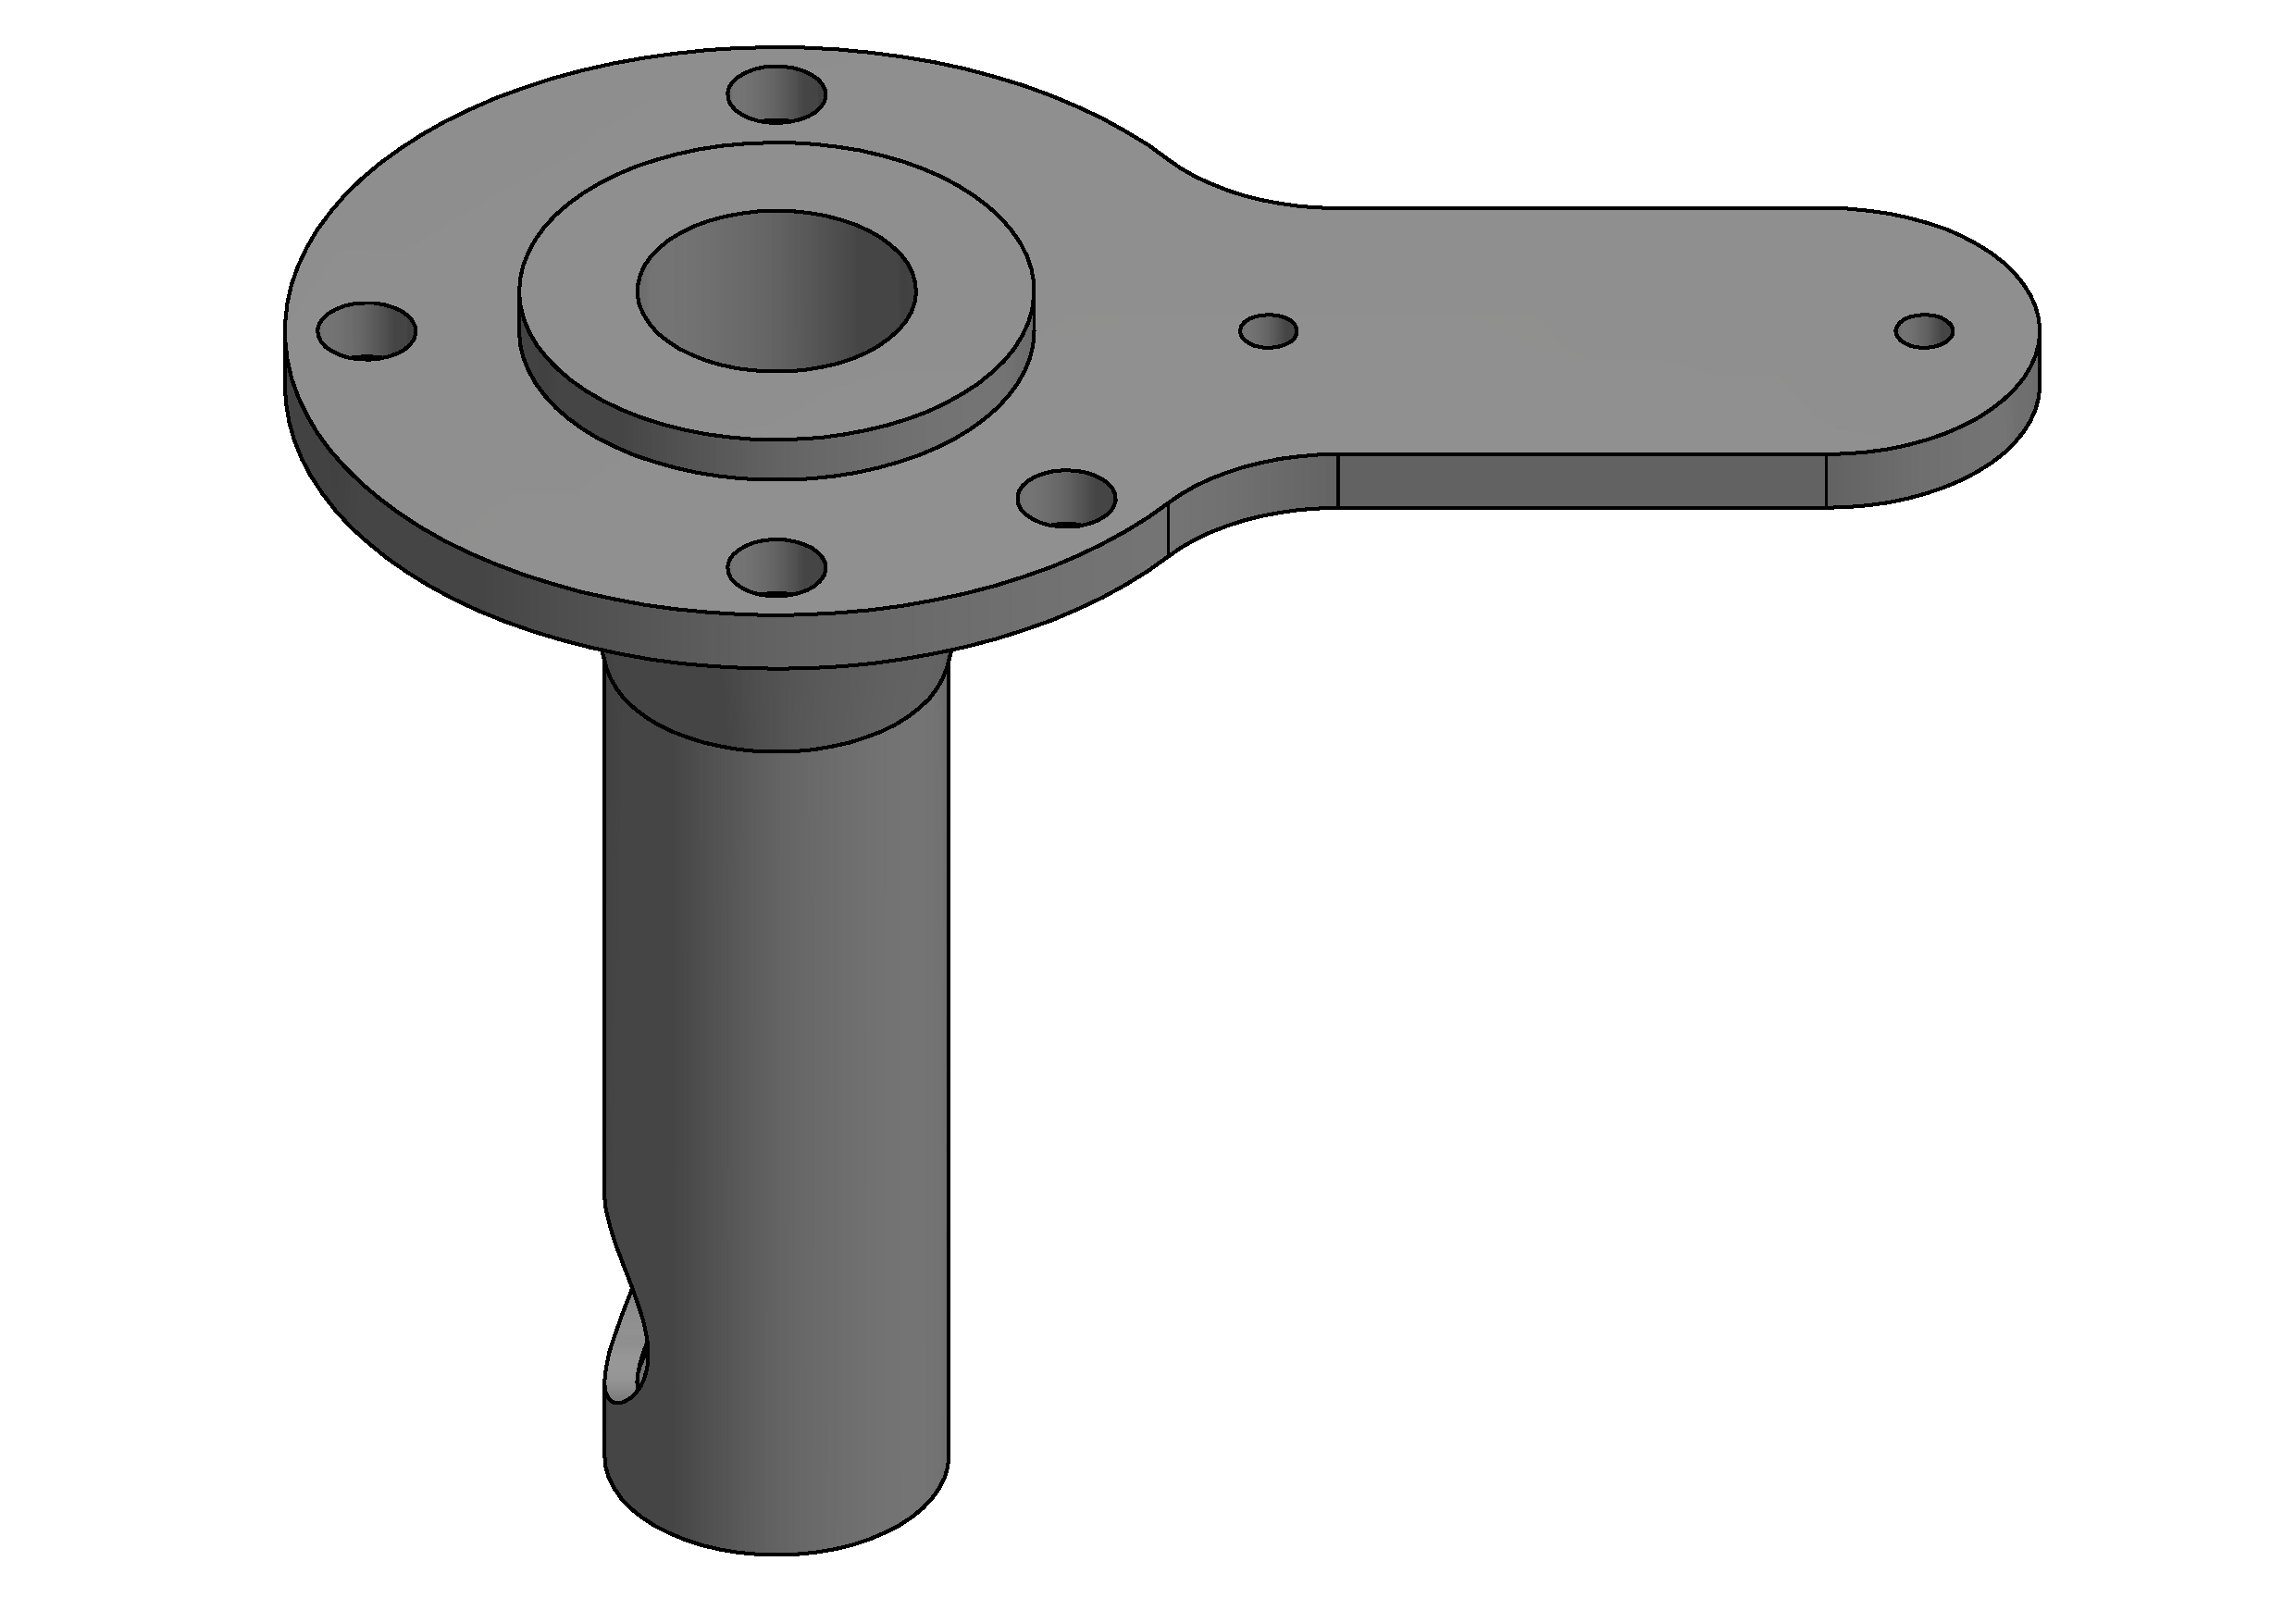
\includegraphics[width=0.48\textwidth]{graphics/single.pdf}}
    \hfill
    \subfloat[Completed end effector mounted on the robot]{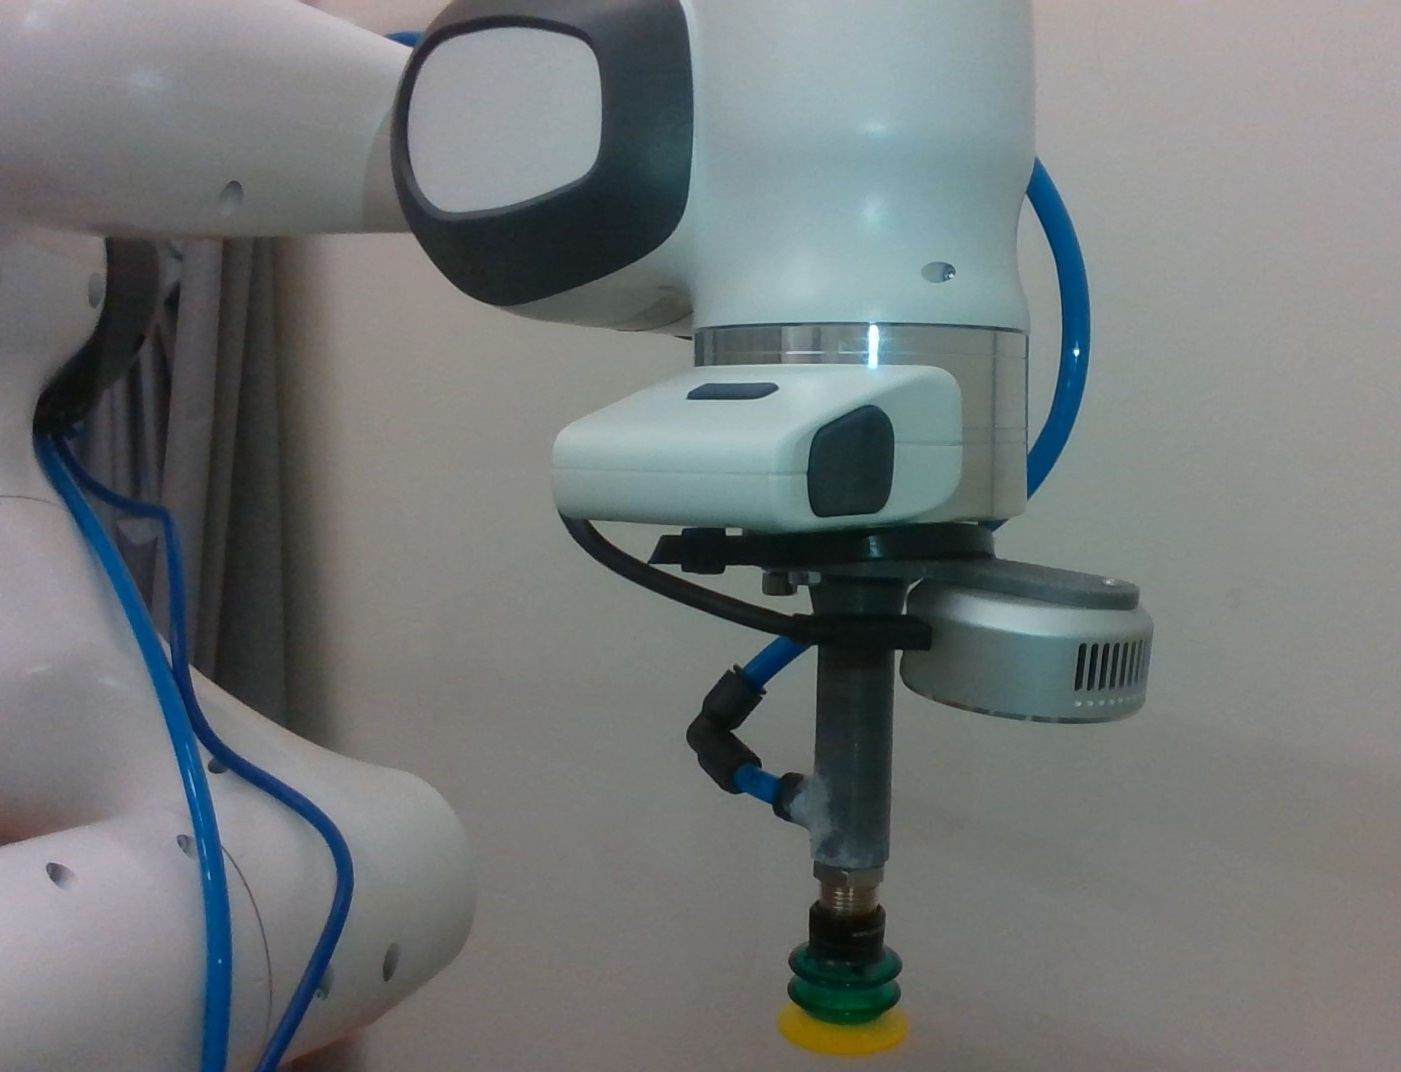
\includegraphics[width=0.48\textwidth]{graphics/endeffector.jpg}}
    %\hfill
    %\subfloat[Real image of the end effector]{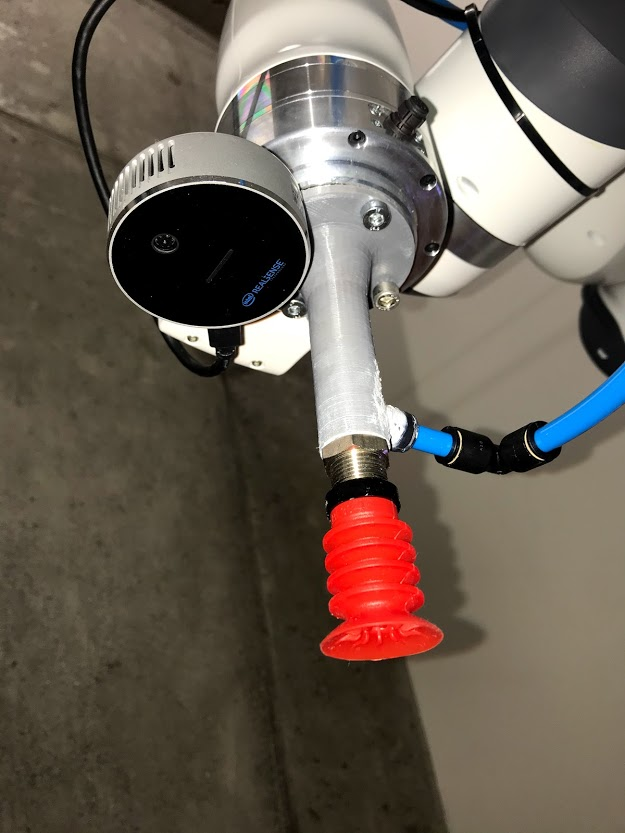
\includegraphics[width=0.25\textwidth]{graphics/rani.jpg}}
    \caption{Robot end effector}
    \label{figure: endeffector}
\end{figure}

\subsection{Camera\label{subsec:camera}} 
In this project, the Intel RealSense LiDAR Camera was used because it generates point clouds with depth information as well as color information from the embedded RGB cameras. LiDAR camera has the potential to provide a dense depth map even in homogeneous areas, where cameras based on passive stereo vision struggle to provide any measurement of depth. The Intel RealSense LiDAR Camera makes use of a proprietary MEMS mirror scanning technology that increases laser power quality. The Intel RealSense LiDAR Camera has a high-resolution FHD RGB camera and an IMU for more reliable handheld scanning. With low power consumption and the ability to produce 23 million precise depth points per second, it's ideal for a wide range of applications. The LiDAR Camera L515 is designed for indoor use with adjustable lighting \cite{noauthor_intel_nodate}.
\begin{figure}[h]
    \centering
    % include first image
    \subfloat[Depth image]{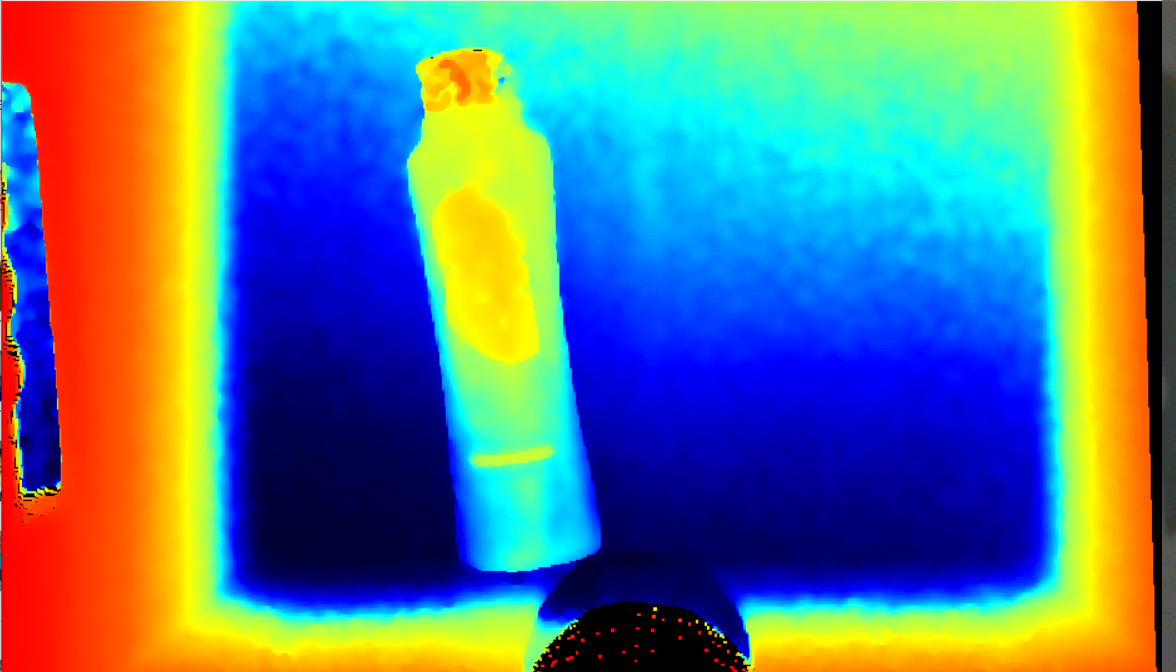
\includegraphics[width=0.33\textwidth,trim={4cm 0 4cm 0},clip]{graphics/methods/depth.png}\label{fig:l515depth}}
    \hfill
    \subfloat[RGB image]{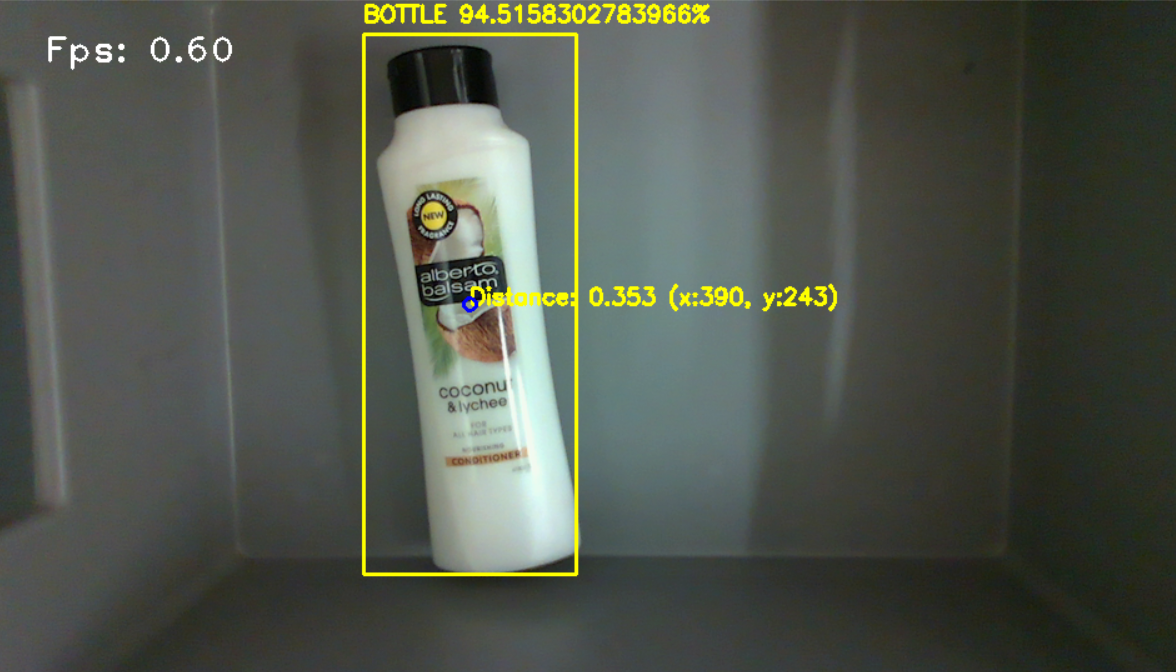
\includegraphics[width=0.33\textwidth,trim={4cm 0 4cm 0},clip]{graphics/methods/color.png}\label{fig:l515color}}
    \hfill
    \subfloat[The camera coordinates system]{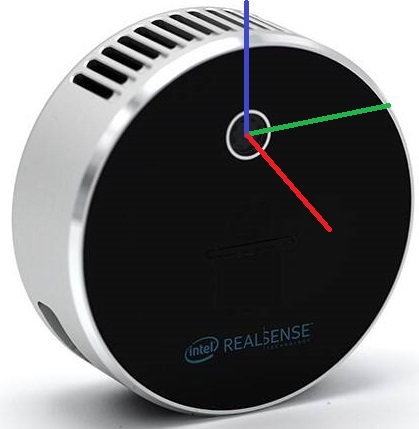
\includegraphics[width=0.3\textwidth]{graphics/lidar515.jpg}\label{fig:l515cor}}
    \caption{Intel RealSense LiDAR Camera L515 \cite{noauthor_intel_nodate}}
    \label{figure: lidar}
\end{figure}
\clearpage

\section{Software implemented for the experiments}
%% \
%\fxfatal{Start by stating what the implemented software is supposed to do and connect this to the objectives.  Then proceed to describe how the software is divided into three components and describe each one in broad terms.}
The software implemented for the project experiments were three codes and one launch file, and were created to answer the research questions. There were implemented two softwares(\textit{pick\_and\_place and find\_pickpoint}) to generate new arrangements of objects using a robot manipulator, and one code to annotate objects automatically, determining the extent of the objects in the images(\textit{difference)}.

The panda\_bringup was used to launch the robot, camera, the suction, and the motion planner\textit{(Sec:\ref{sec:pandabringup})}. 
The pick\_and\_place code controls the robot \textit{(Sec:\ref{sec:robot})}, find\_pickpoint which talks to the camera and uses data to locate items \textit{(Sec:\ref{camera})} and then the difference which finds the difference between before and after picture and labels the images \textit{(Sec:\ref{labelimg})}.

\begin{figure}[h]
    \centering
    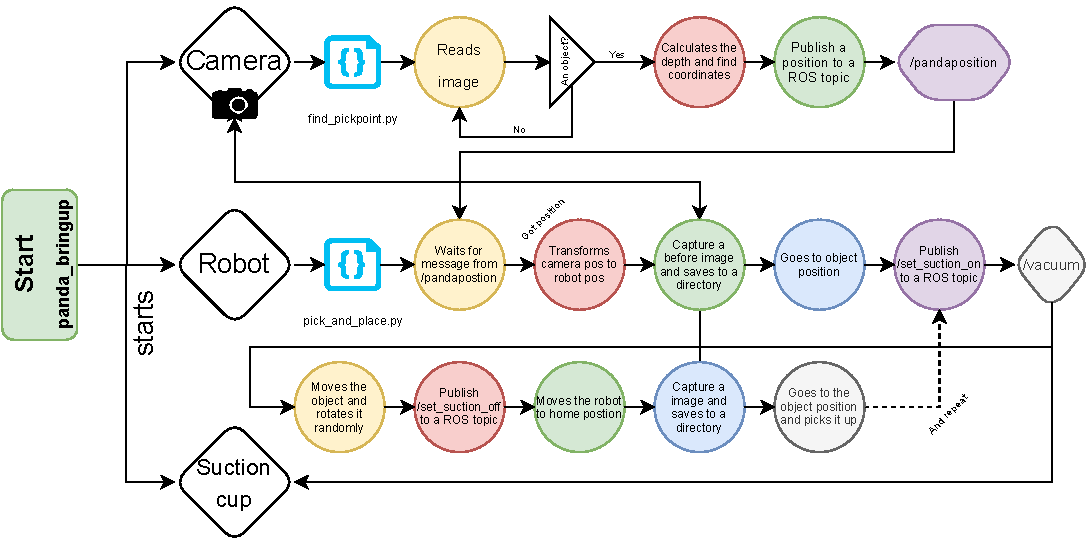
\includegraphics[width=0.9\textwidth]{graphics/softwareDiagram.pdf}
    \caption{Software diagram that shows how the panda\_bringup works}
    \label{fig:softwarediagram}
\end{figure}

A summary of the software diagram, the camera reads images and calculates the depth, the robot picks the object at the desired position and moves it to another position and the suction cup takes commands from the robot.

\subsection{Automatic generation of training images}\label{sec:robot}
Two versions of software were created to control the robot. One that only moved one object around inside of the bin and captured images, this version was used when the bin had one object in the bin. The second version picked up one object and moved that object to another bin, this version was used when the bin had multiple object in the bin.

The robot manipulator was programmed in python and used ROS to communicate with the robot, the two versions of the software can be found in the \textit{Appendix \ref{sec:pickandplace}} and \textit{Appendix \ref{sec:v2pickandplace}}, known as \textit{pick\_and\_place.py} and \textit{v2pick\_and\_place.py}. 
Both versions of the software, start by creating two ROS publishers, one that talks to the Festo vacuum suction cup and the other that talks to the MoveIt! motion planner. 
It also to creates a TF(transform) listener so it is possible to read the current positions and orientations, also it can transform poses between the coordinate frames attached to each link of the robot. The robot coordinates system is explained in \textit{Figure \ref{fig:pandachain}} 

\subsubsection{Training images with one object in the bin}\label{robotcontrol}
This version is the first version of the software, and it moves one object inside of the bin. The software has an loop that runs while ROS is running. 
Where the robot waits for a message from the find\_pickpoint.py through a ROS topic where it gets an object position from the camera.
The TF listener then transforms the object position in camera coordinates to world coordinates. The robots then move to the object position and pick up the object using the suction cup. When the robot has picked up the object successfully it moves the object to another position and rotates the object by a random amount. When the robot has successfully moved the object it goes to the fixed home position and takes an image and saves it into a directory. 

\begin{figure}[h]
    \centering
    % include first image
    \subfloat[Starts in home position and capture an image]{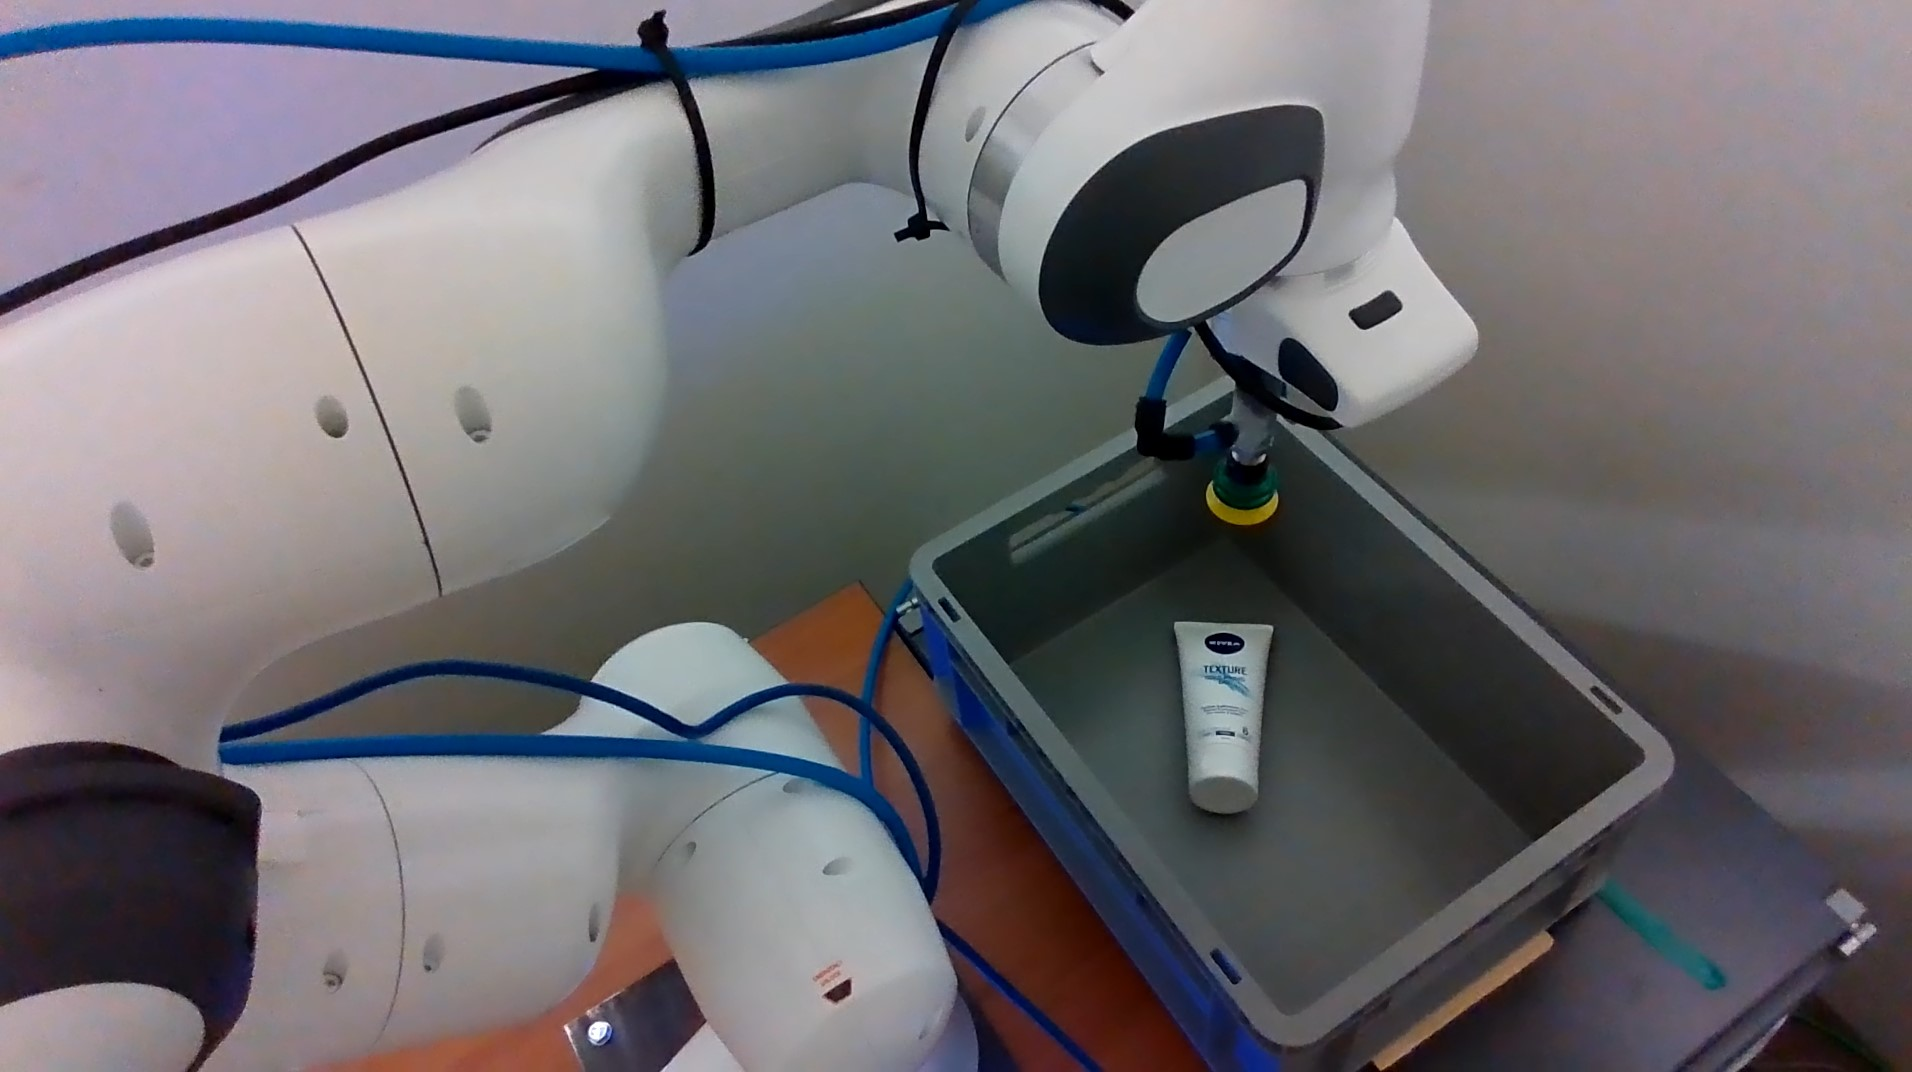
\includegraphics[width=0.33\textwidth]{graphics/results/1home.jpg}}
    \hfill
    \subfloat[Goes to the object]{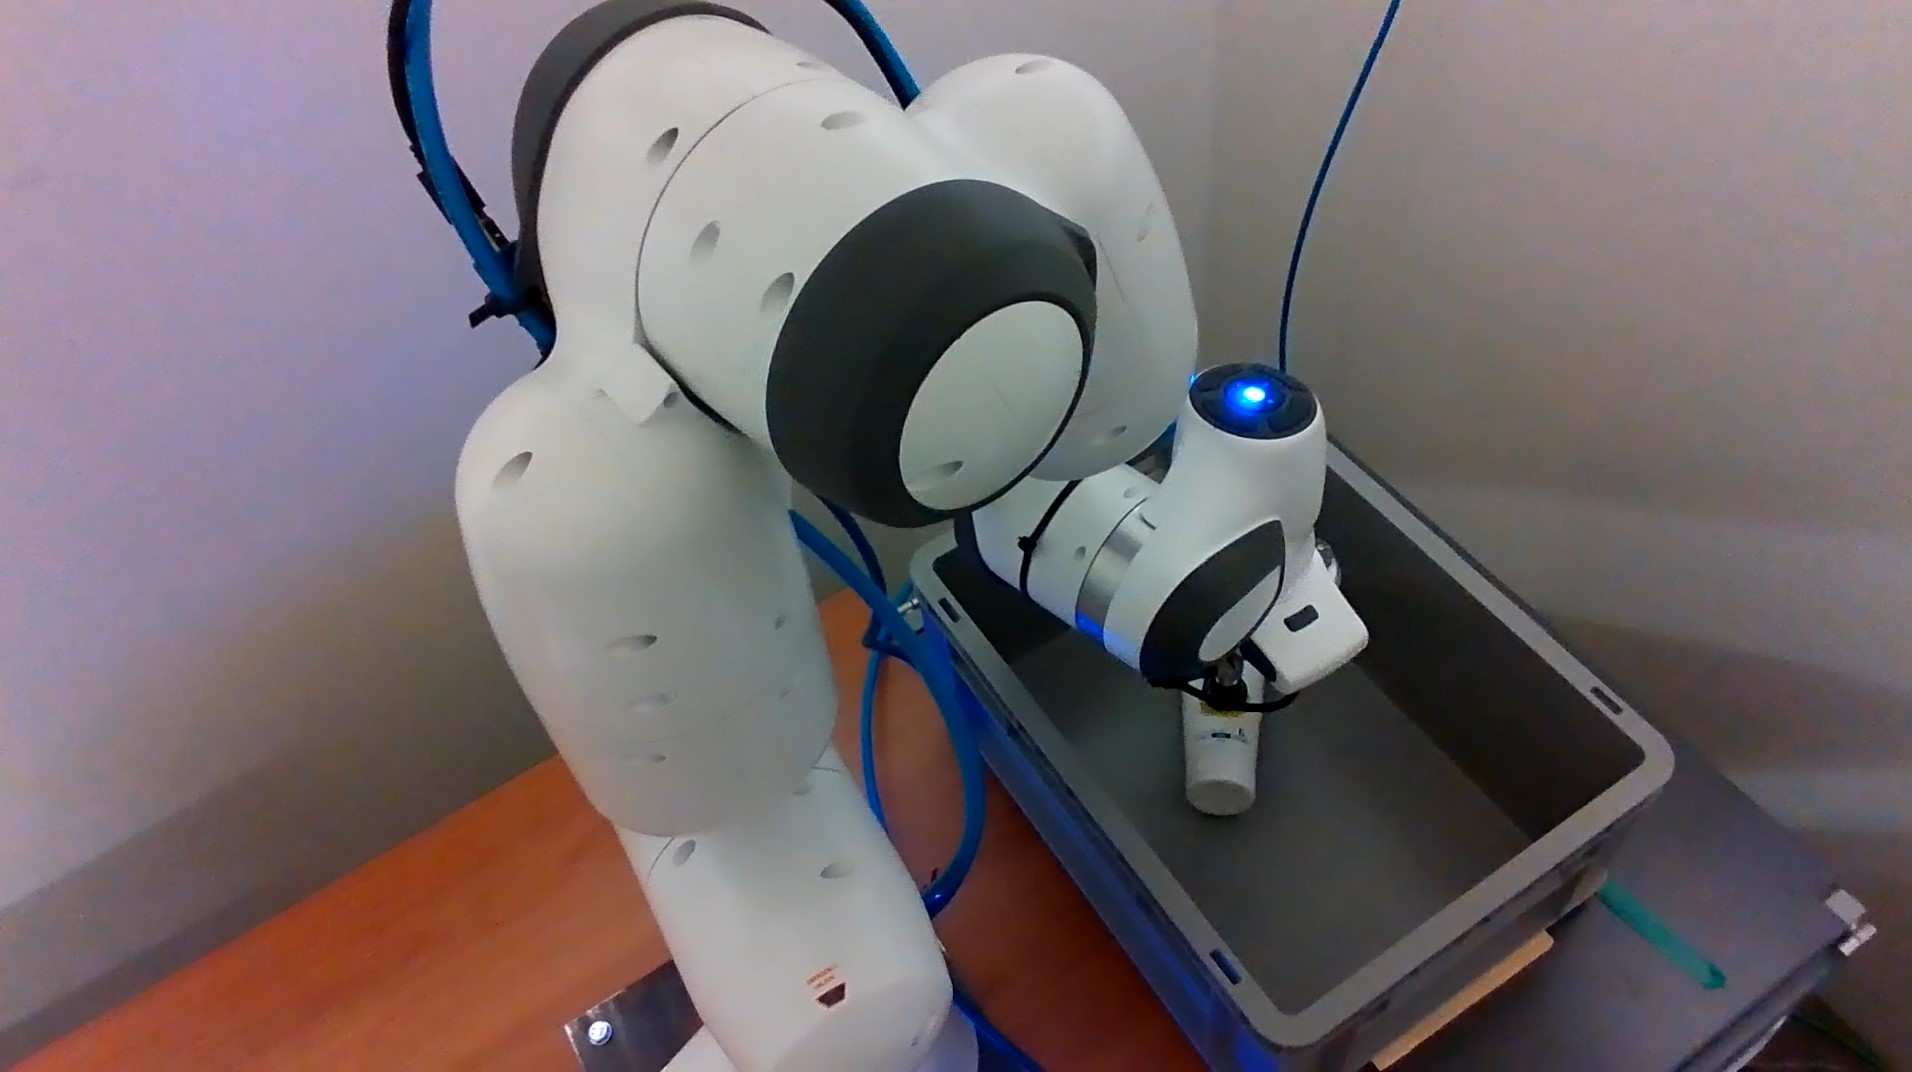
\includegraphics[width=0.33\textwidth]{graphics/results/2pick.jpg}}
    \hfill
    \subfloat[Picks up the object]{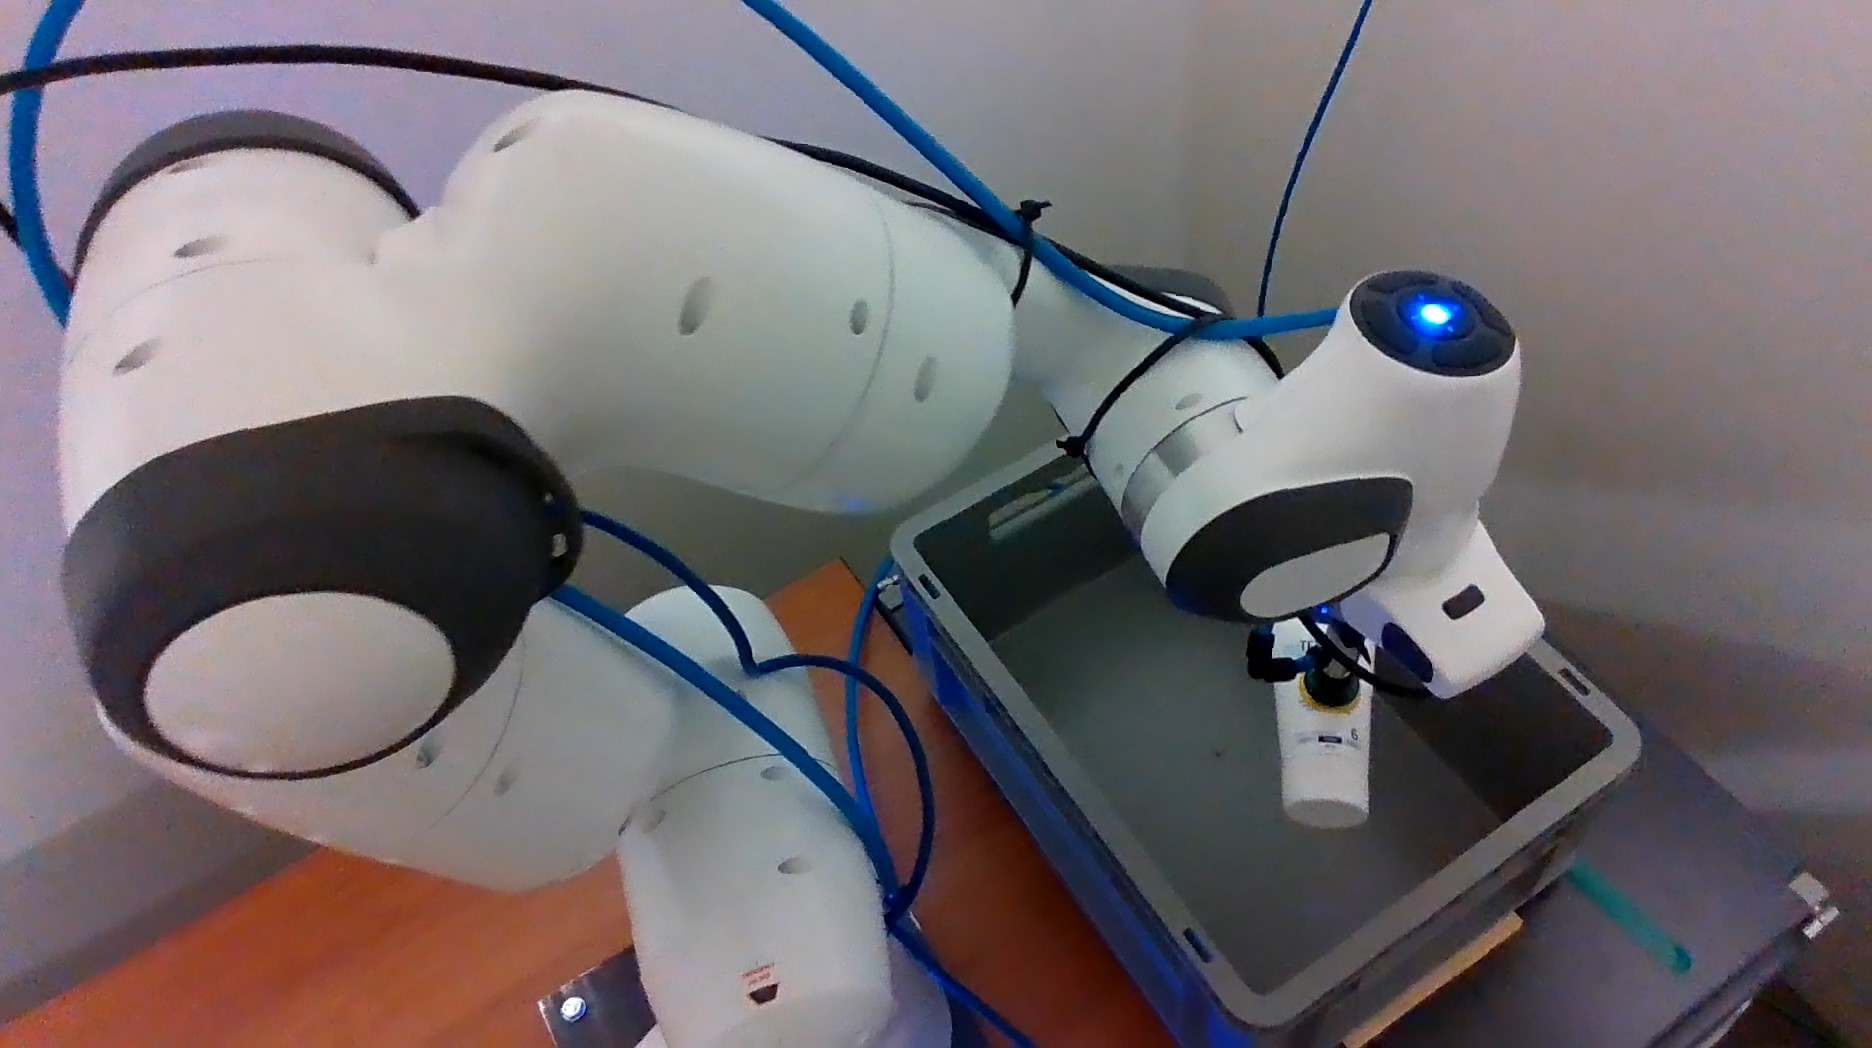
\includegraphics[width=0.33\textwidth]{graphics/results/3move.jpg}}
    \hfill
    \subfloat[Moves the object to another position]{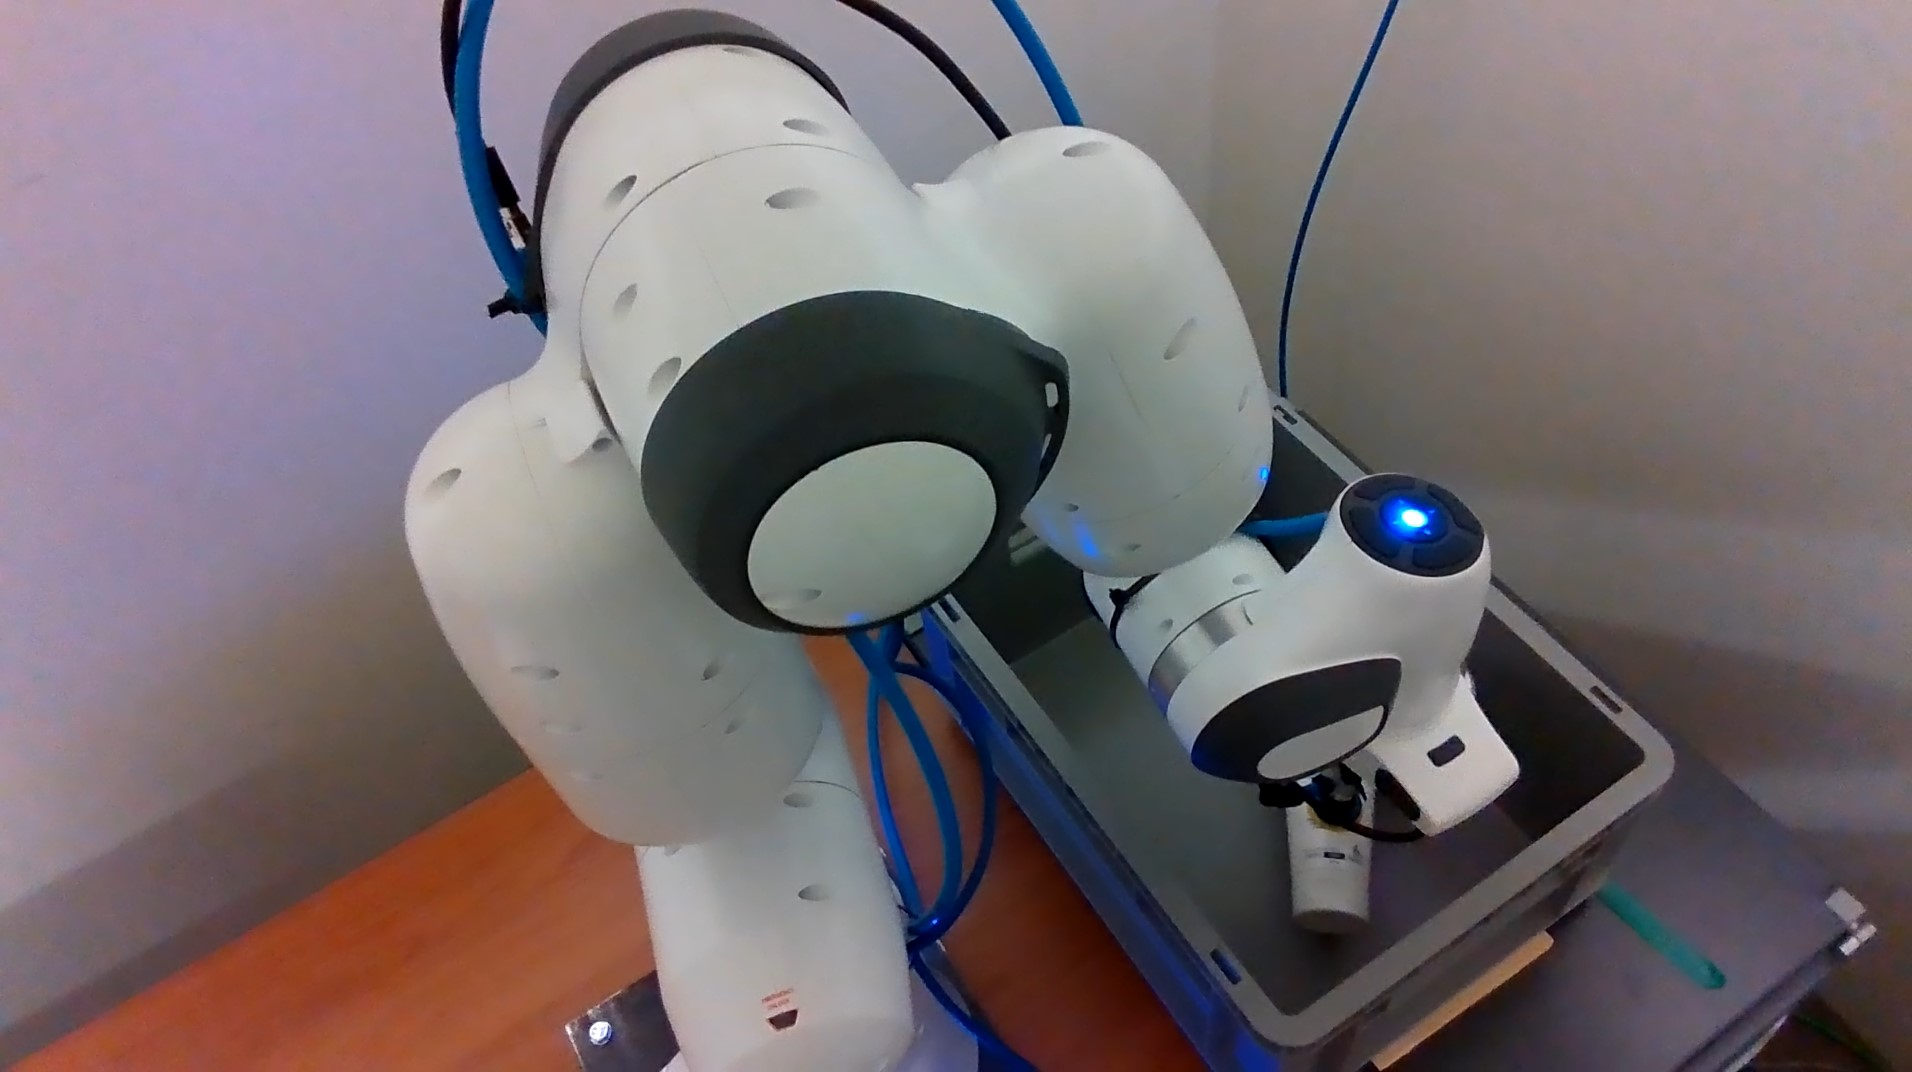
\includegraphics[width=0.33\textwidth]{graphics/results/4above.jpg}}
    \hfill
    \subfloat[Rotates the object and drops it]{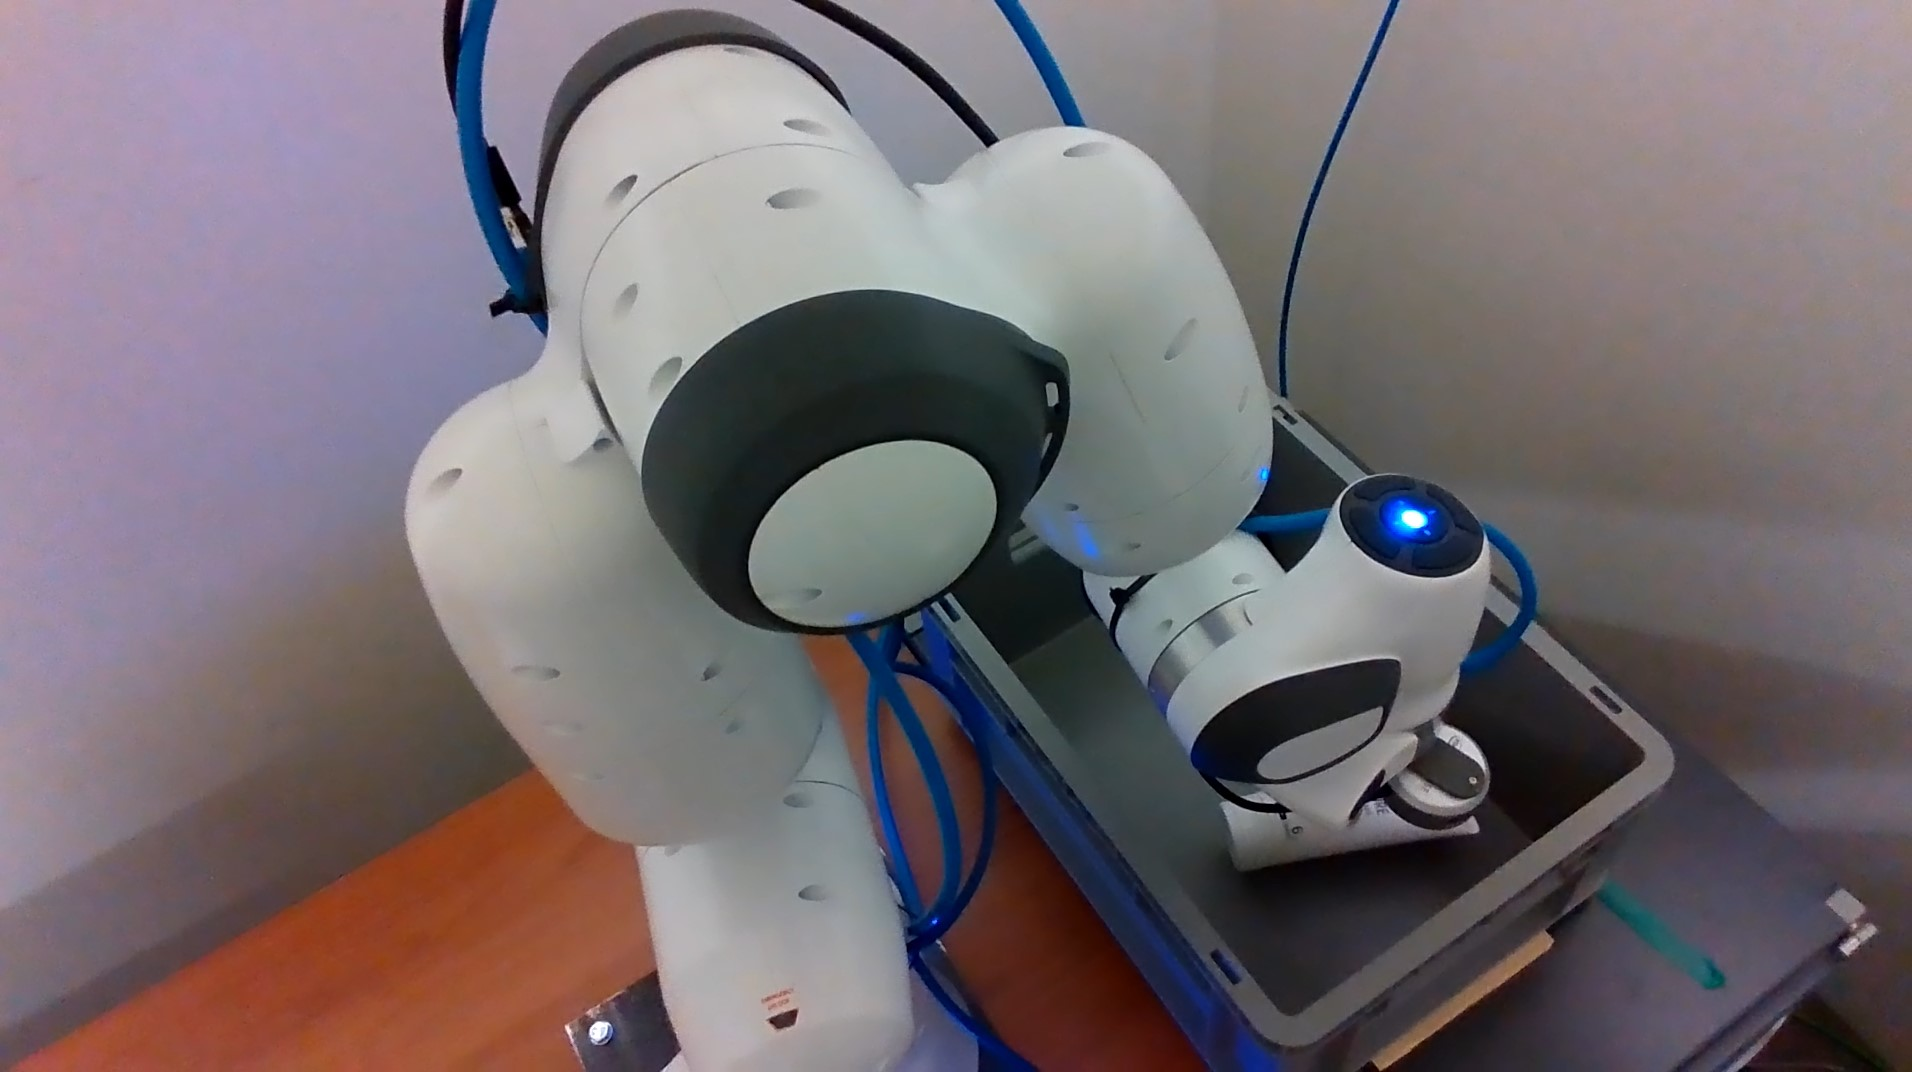
\includegraphics[width=0.33\textwidth]{graphics/results/6rotate.jpg}}
    \hfill
    \subfloat[Goes to home position and capture another image]{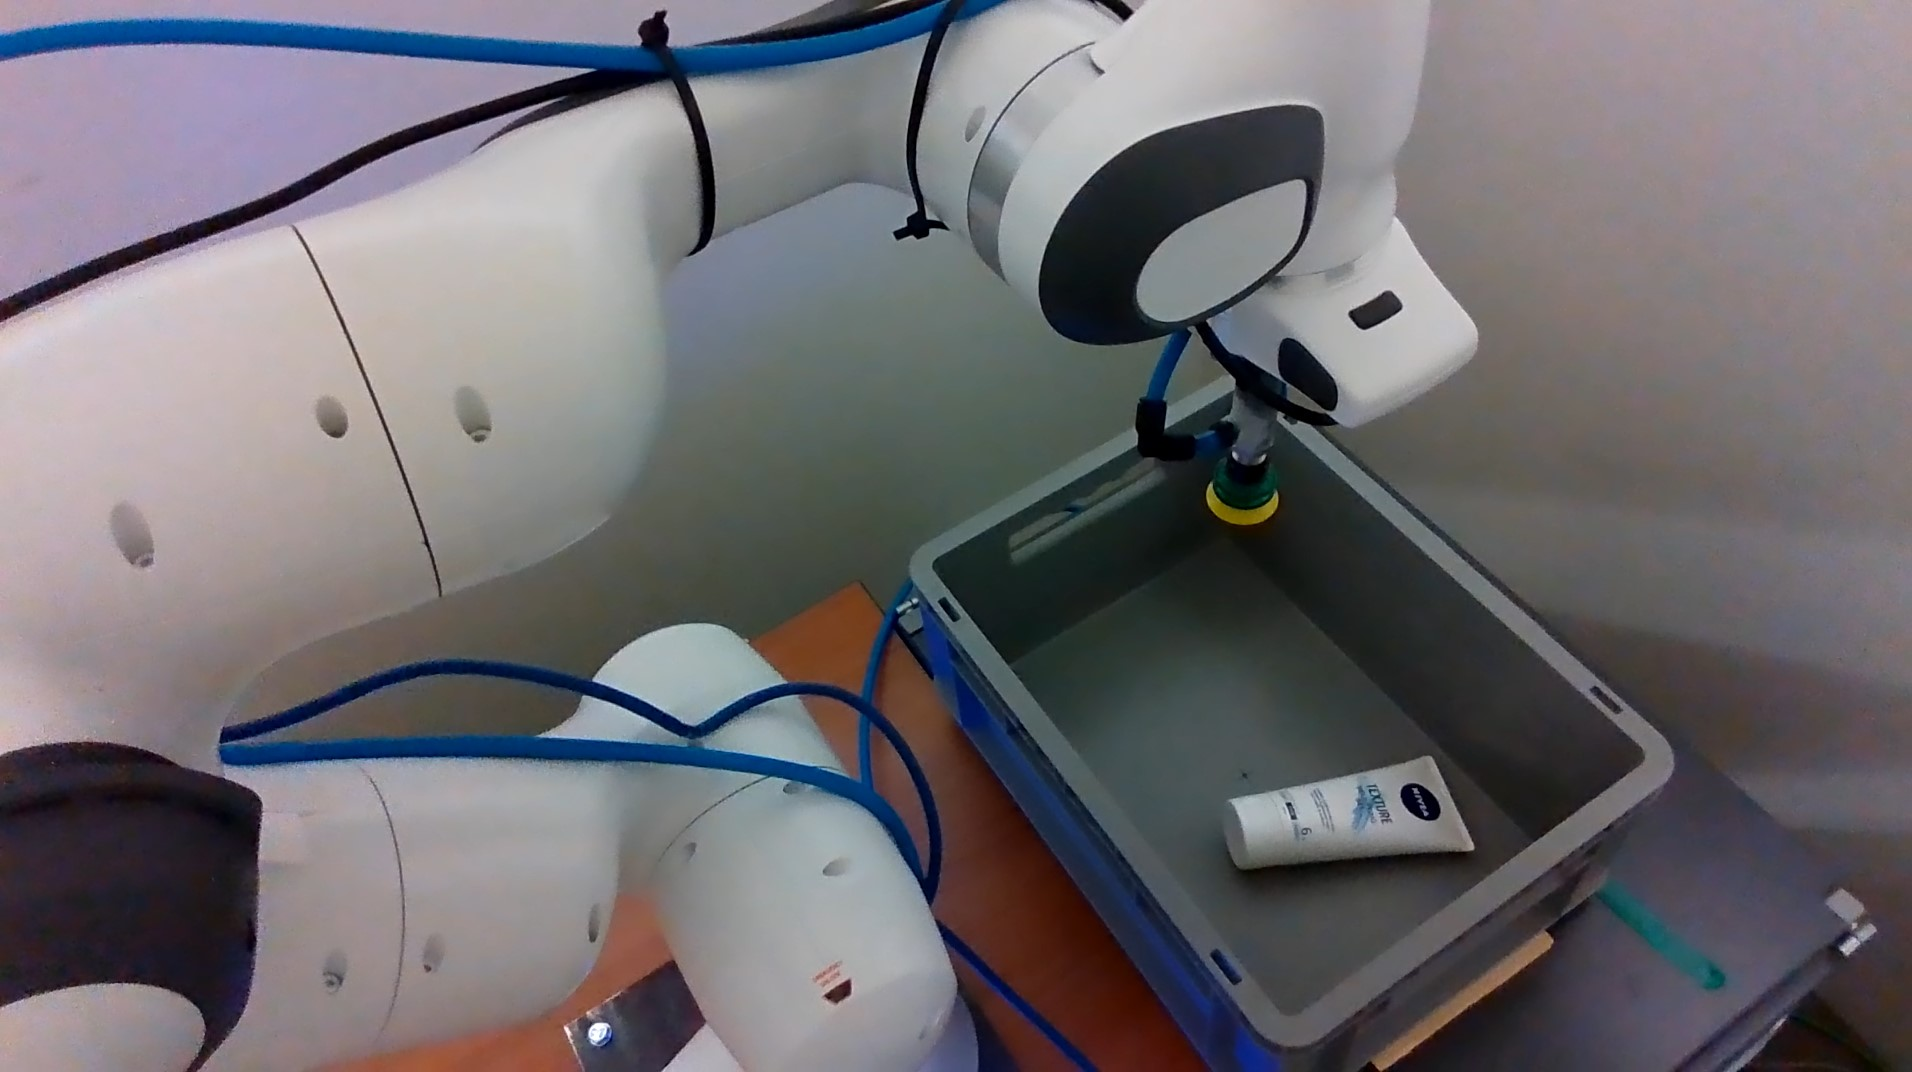
\includegraphics[width=0.33\textwidth]{graphics/results/5drop.jpg}}
    \caption{How the robots works}
    \label{figure: robotworking}
\end{figure}

\subsubsection{Training images with multiple objects in the bin}
This version is the second version of the software, and it picks up one object inside of the bin and moves it to another bin.


% The software has an loop that runs while ROS is running. 
% Where the robot waits for a message from the find\_pickpoint.py through a ROS topic where it gets an object position from the camera.
% The TF listener then transforms the object position in camera coordinates to world coordinates. The robots then move to the object position and pick up the object using the suction cup. When the robot has picked up the object successfully it moves the object to another position and rotates the object by a random amount. When the robot has successfully moved the object it goes to the fixed home position and takes an image and saves it into a directory. 
\fxfatal{skrifa }


\subsection{Image collection and visual guidance}\label{camera}
%\fxfatal{Also make sure that you state clearly that you start from an initial arrangement, in which the object can be detected by the current model, and then proceed to generate (and label) novel arrangements, some of which are not handled by the current model.}
The camera was used to find the pick point of an object and it was coded in Python and used ROS communication, the code can be found in the \textit{Appendix \ref{sec:findpickpoint}} known as \textit{find\_pickpoint.py}. 
The program starts by initializing a CVBridge class so it can work on images with OpenCV. It then initializes a neural network, so it can find objects in an image. At last, it creates a subscriber to the "/camera/color/image\_raw" topic with the function "image\_callback" as a callback and creates a publisher "pandaposition" that talks to the robot manipulator. Then a loop keeps the program from shutting down unless ROS is shut down.

When the callback gets an image it waits for an aligned depth to a color image so it can read a depth at a certain point. It then goes into a find objects function that finds the object in the image using the neural network, which locates the center of an object. When the program has found pixel coordinates of the object it can find the depth at that point and can create real-world coordinates(X, Y, Z) in meters at the camera location. At last, the programs send the real-world coordinates to a "pandaposition" publisher so the robot manipulator uses the coordinates.

\begin{figure}[h]
    \centering
    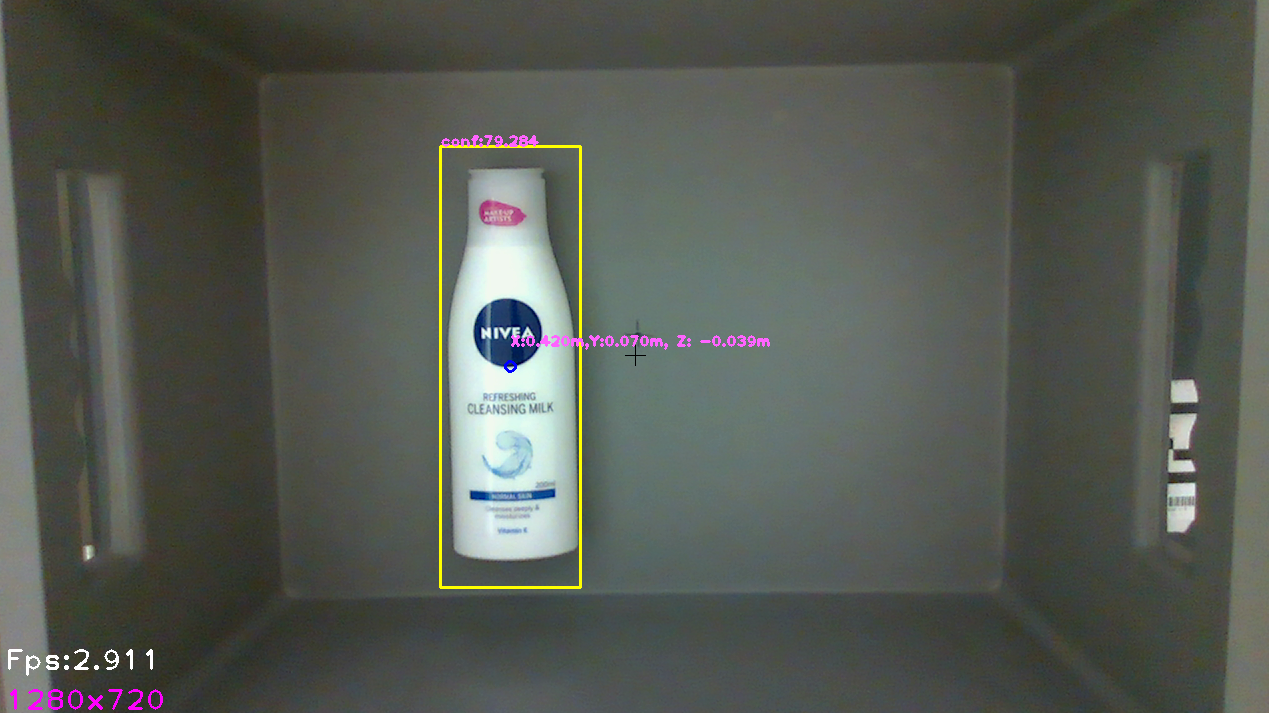
\includegraphics[width=0.8\textwidth]{graphics/findpickpoint.png}
    \caption{An example of the output from the find\_pickpoint.py code}
    \label{fig:findpickpoint}
\end{figure}

From \textit{Figure \ref{fig:findpickpoint}} you can see the confidence, frames per second(Fps), image size, X which is forward length or depth, Y and Z is the distance from the center of the camera in meters. 
The camera coordinates system can been seen in \textit{Figure \ref{fig:l515cor}}.


\subsection{Automatic image labelling}\label{labelimg}
When the robot manipulator and camera had captured images from a fixed home position, the images were put in a software called \textit{difference.py} which finds the difference between images, and can be found in the \textit{Appendix \ref{sec:difference}}. That program was coded in Python and works individually. The program locates objects in the images and labels them. 
\subsubsection*{Before vs. After}\label{beforeandafter}
The first method used before- and after- image, the bottle was moved to the other side and then found the difference. It calculates the Structural Similarity Index (SSIM) between the two images, SSIM\cite{datta_all_2021} is used as a metric to measure the similarity between two given images. The OpenCV threshold and contours were used to draw the contours. Then iterate around the contour area, and get a bounding area and draw a rectangle around.
An example of input images can been seen in \textit{Figure \ref{figure: beforeafter}}, and try's to find the difference between before and after.
\begin{figure}[h]
    \centering
    % include first image
    \subfloat[Before]{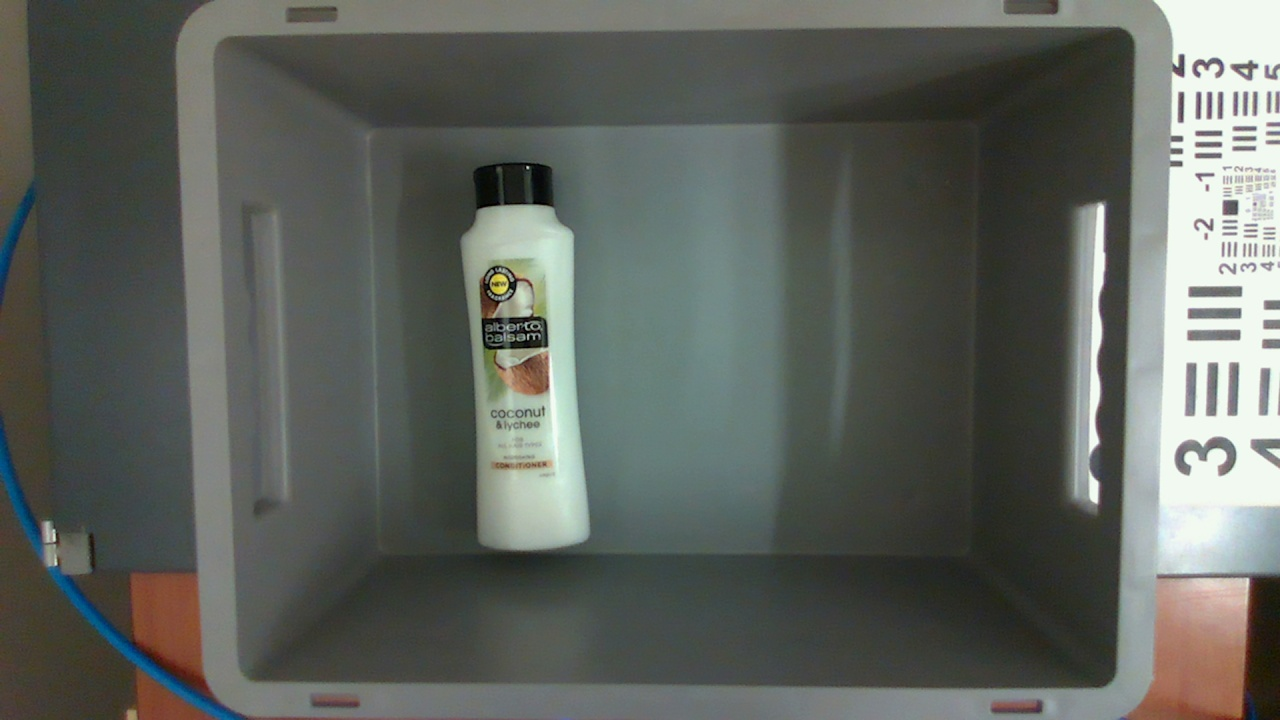
\includegraphics[width=0.45\textwidth]{graphics/methods/frame0000.jpg}}
    \hfill
    \subfloat[After]{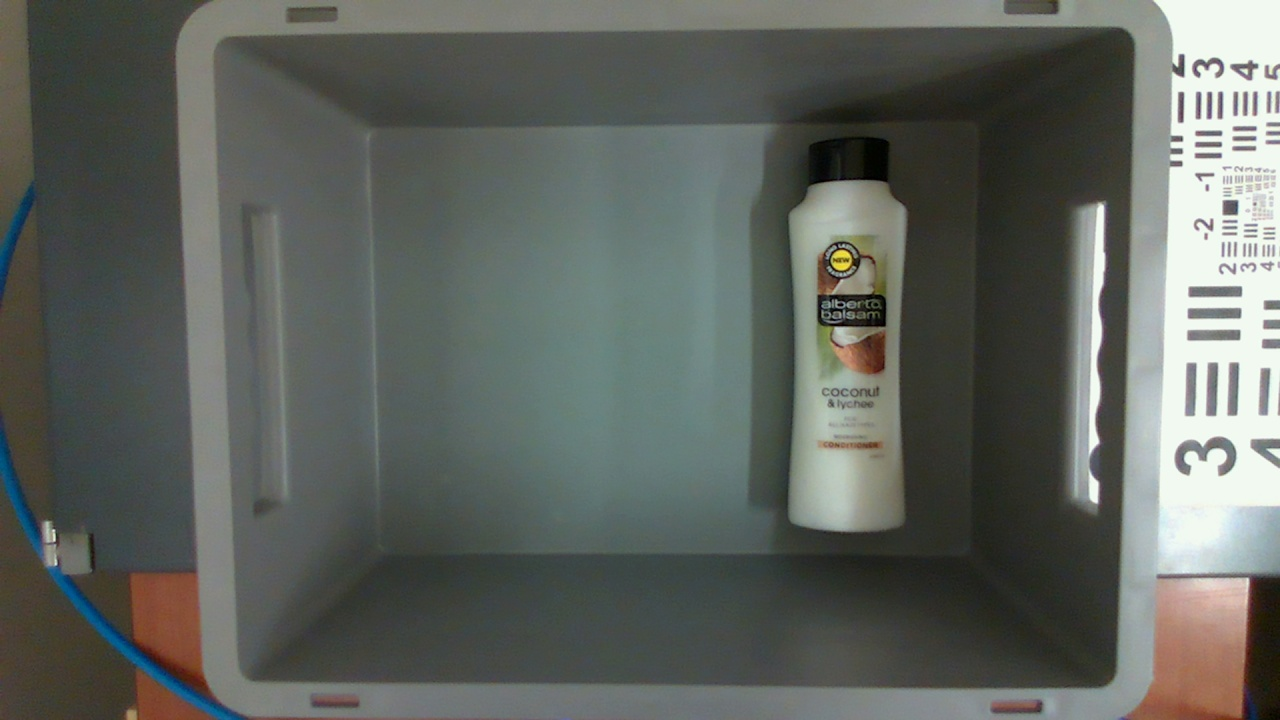
\includegraphics[width=0.45\textwidth]{graphics/methods/frame0001.jpg}}
    \caption{An example of input images}
    \label{figure: beforeafter}
\end{figure}

\subsubsection*{Empty bin vs. item in the bin}\label{emptyvsitem}
The second method uses two functions to find objects in the image, one is to find the difference between an empty bin and a bin with an object inside and the other is to find contours in the image. 
The function that delivers better results is used or if the results are similar average values are used. 
In this program, OpenCV and Skicit-image are used. 
So the program starts by getting an image of an empty bin and then the images with an object in it. 
Then it finds uses \textit{cv2.Canny} to find the edges, creates a binary threshold image with \textit{cv2.threshold} and finds the contours from the threshold image.  
When the contours have been found it goes to a function that checks if the contour has four corners to check if it is a rectangle. 
If it has four corners and the area is within area marks it saves the location\textit{(center point, width, and height relative to the image size)} of the object in a text file named the same as the image. 
When the program has finished with the all images an text file with locations of objects for each image, is saved and can be used to train the neural network. An example of input images can been seen in \textit{Figure \ref{figure: emptyafter}}.
\begin{figure}[h]
    \centering
    % include first image
    \subfloat[Empty bin]{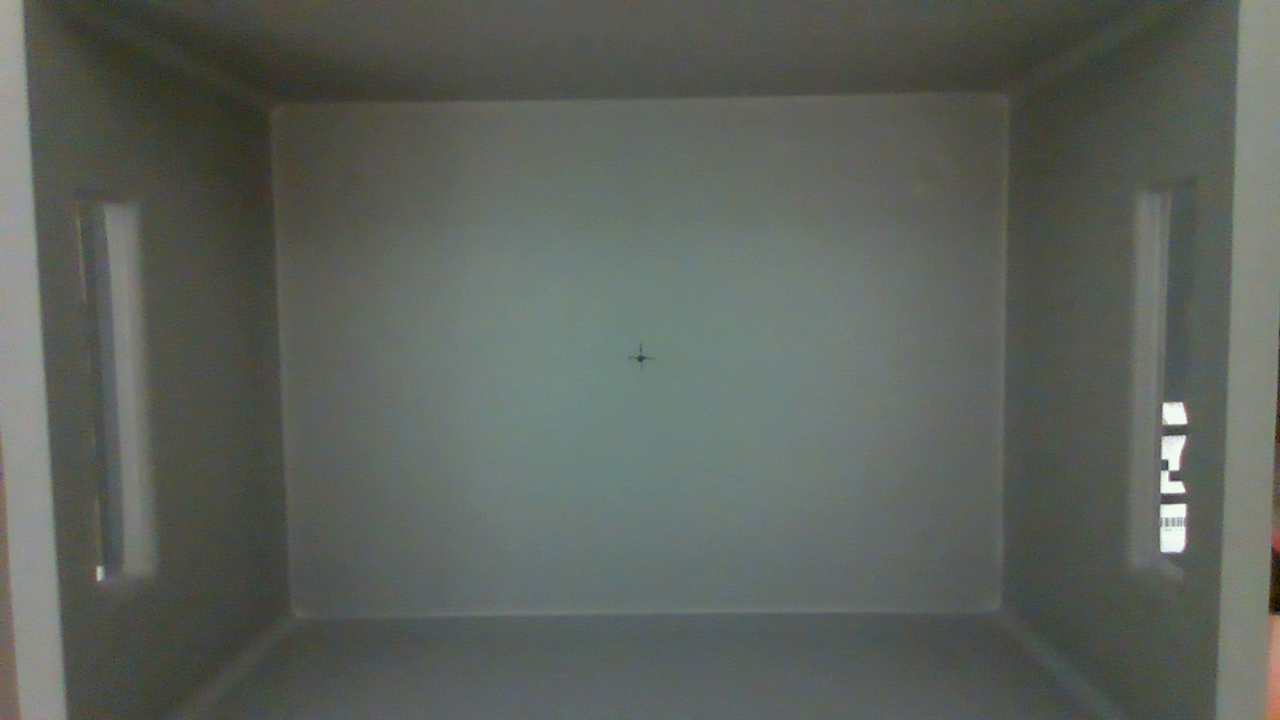
\includegraphics[width=0.45\textwidth]{graphics/methods/0000.png}}
    \hfill
    \subfloat[Item in the bin]{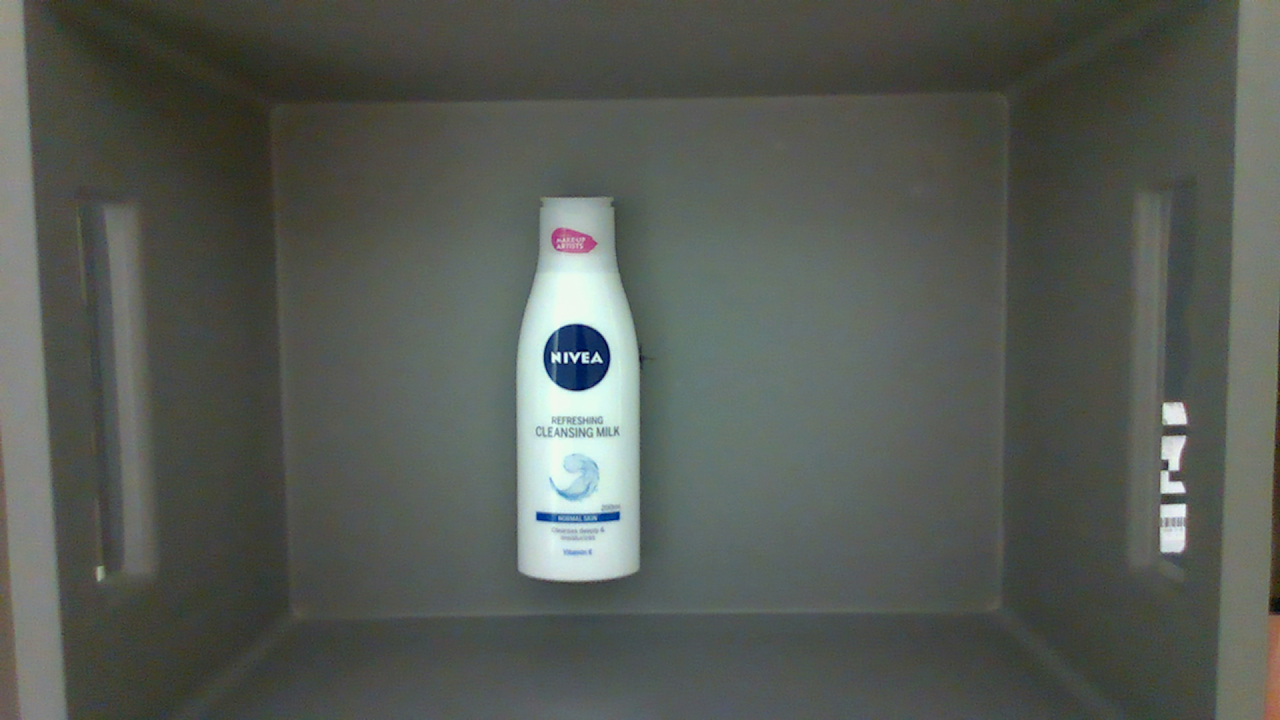
\includegraphics[width=0.45\textwidth]{graphics/methods/0001.png}}
    \caption{An example of input images}
    \label{figure: emptyafter}
\end{figure}
\clearpage
\section{Dataset}
Annotated datasets are intended to add metadata to a dataset. The metadata is normally tagged. Tags may be added to any data type, including texts, images and videos. There are many ready-made datasets online such as the COCO - Common objects in context \cite{noauthor_coco_nodate} and Google’s Open Images dataset \cite{noauthor_open_nodate}.

Most ready-made datasets for object detection are better suited for self-driving cars and image classification. They focus more on items such as, people, animals and large objects such as cars and bikes. For this project, the emphasis was on object that are sold at online retails stores.
\subsection{Automatically generated dataset with one object in the bin} \label{sec:firstdataset}
The first dataset was made out of bottles which were available in the team’s research department in the basement at Reykjavik University. It included 4 types of products and consists of 376 images, \textit{Alberto Balsam}(101 images), \textit{Nivea Cleansing Milk}(102 images), \textit{Nivea Elastic}(72 images) and \textit{Nivea Texture}(101 images). 
This is a robot-generated dataset with automatically generated labels, which has only one object in the bin. 
These products were moved, rotated and then captured in home position to achieve more images to add to the dataset. 
These products can be seen in \textit{Figure \ref{figure: products}}.

\begin{figure}[h]
    \centering
    % include first image
    \subfloat[Alberto Balsam ]{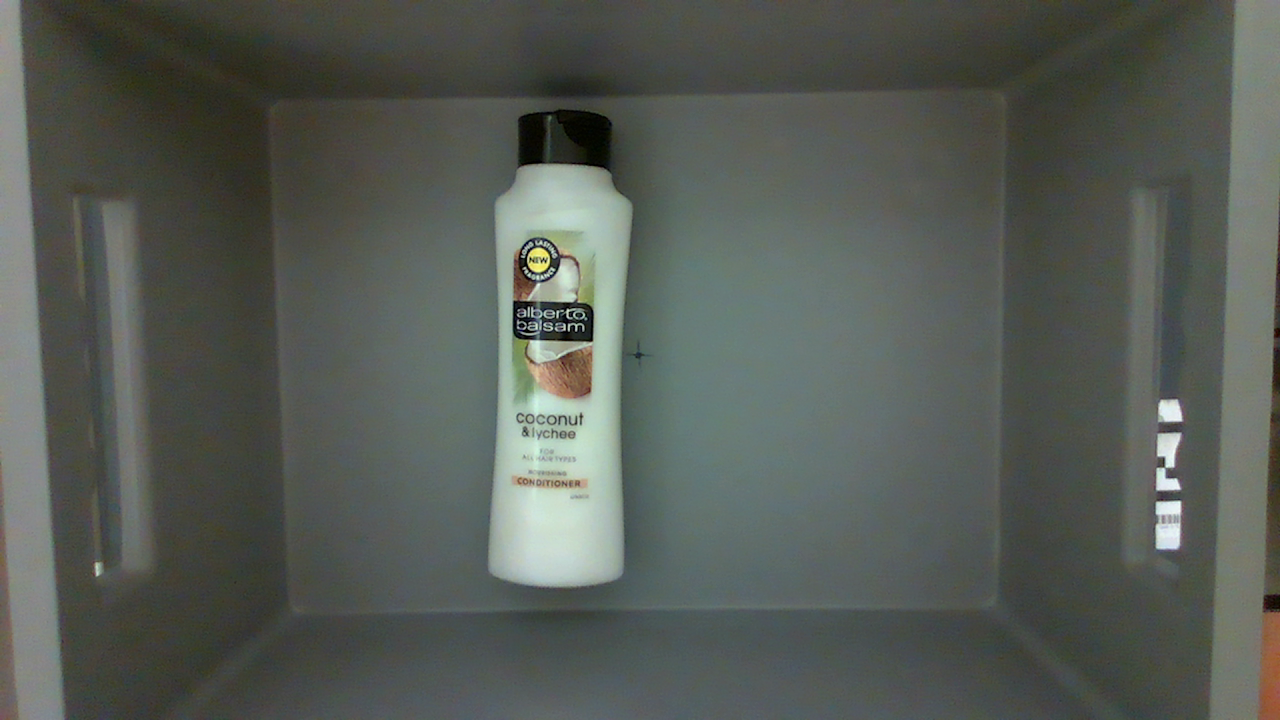
\includegraphics[width=0.37\textwidth]{graphics/methods/b0001.png}}
    %\hfill
    \hspace{2 cm}
    \subfloat[Nivea Cleansing Milk]{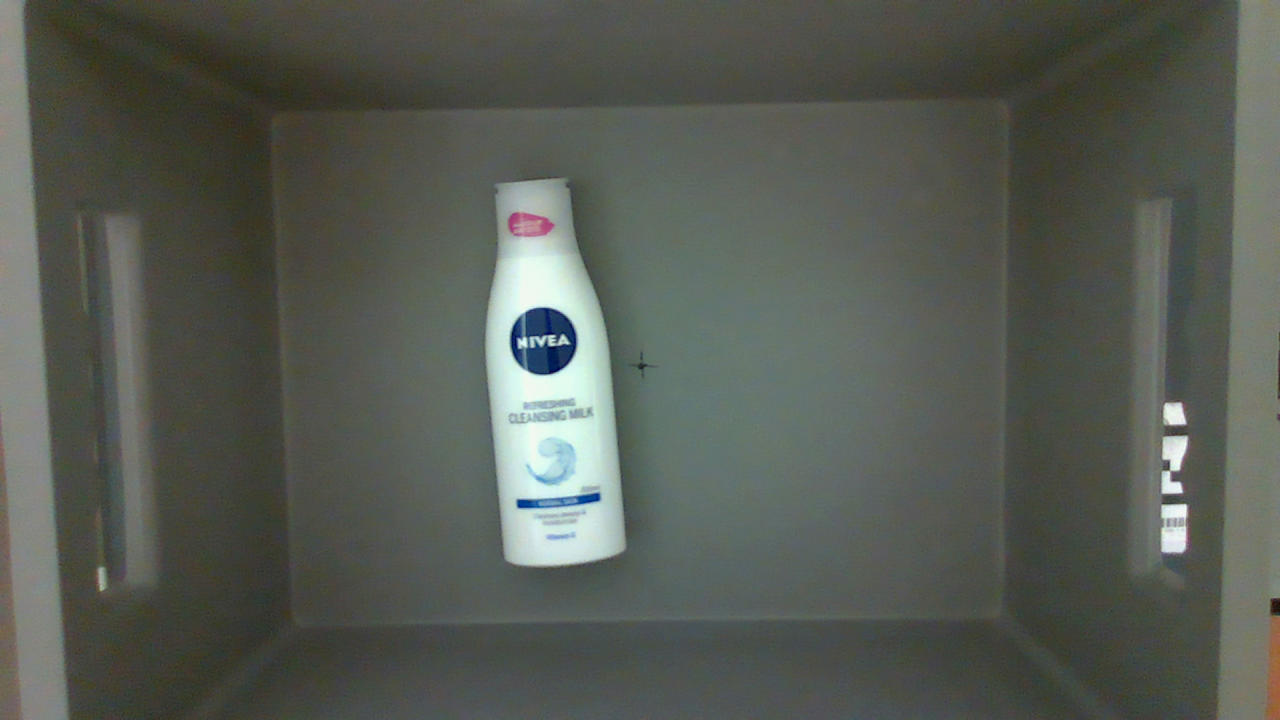
\includegraphics[width=0.37\textwidth]{graphics/methods/b0144.png}}
    %\hfill
    \hspace{2 cm}
    \subfloat[Nivea Elastic]{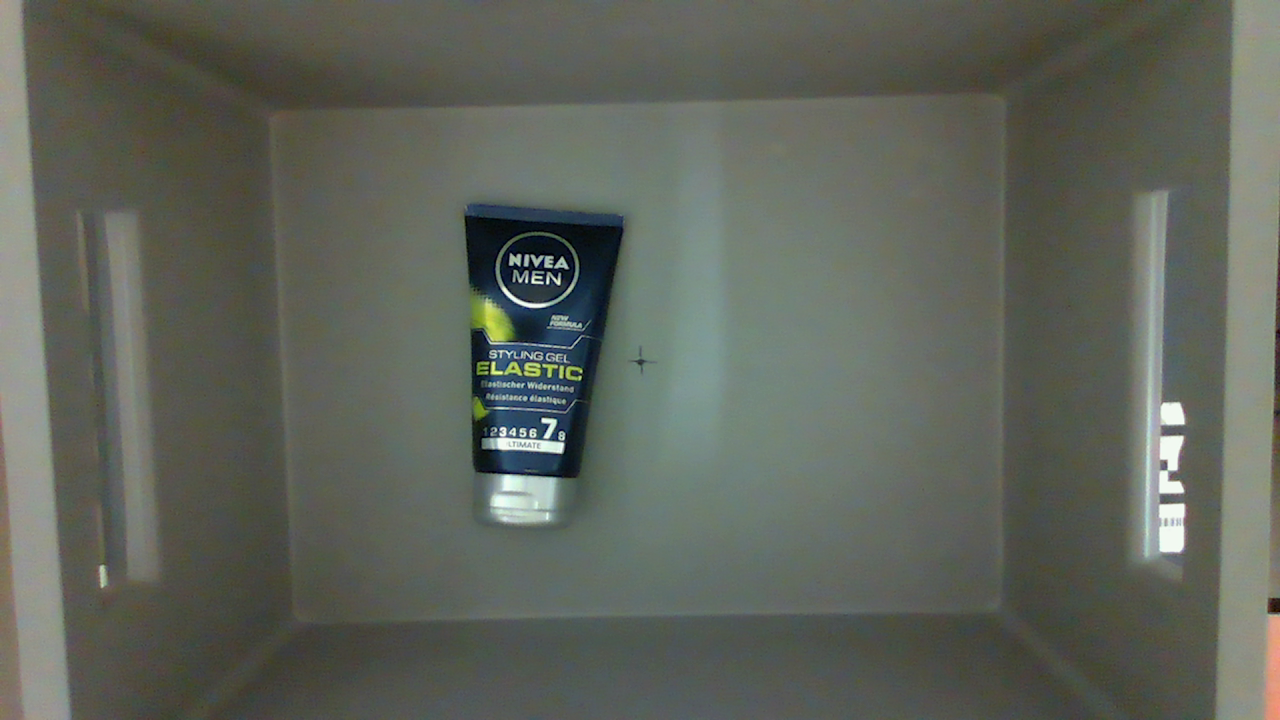
\includegraphics[width=0.37\textwidth]{graphics/methods/b0209.png}}
    %\hfill
    \hspace{2 cm}
    \subfloat[Nivea Texture]{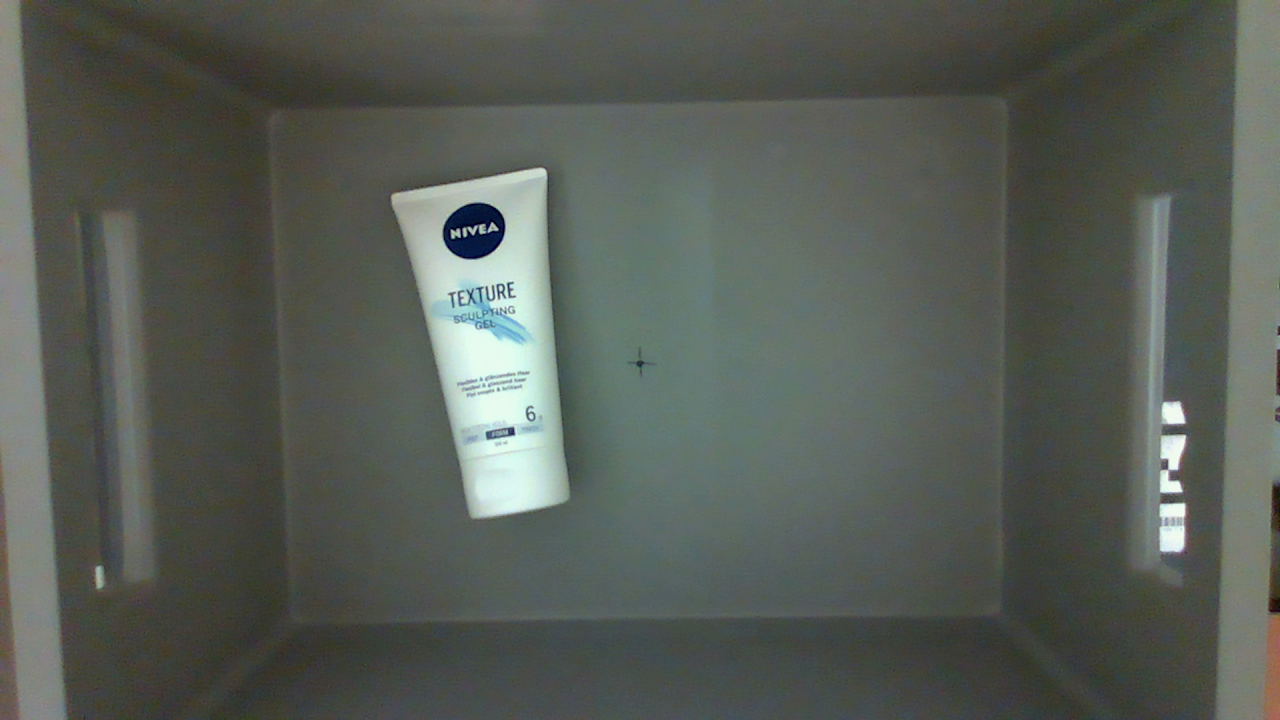
\includegraphics[width=0.37\textwidth]{graphics/methods/b0358.png}}
    \caption{The first dataset contained 4 products, with only one object in the bin}
    \label{figure: products}
\end{figure}

\subsection{Automatically generated dataset with multiple objects in the bin} \label{sec:multidataset}
The first dataset was made out of bottles which were available in the team’s research department in the basement at Reykjavik University. It included 4 types of products and consists of 72 images, \textit{Alberto Balsam}(18 images), \textit{Nivea Cleansing Milk}(18 images), \textit{Nivea Elastic}(18 images) and \textit{Nivea Texture}(18 images). 
This is a robot-generated dataset with automatically generated labels, which has multiple objects in the bin. 
These objects were picked up and moved to another box. When the robot had moved the object to another bin an image was captured of the items bin in an fixed home position and  added to the dataset. Then it was possible to find an difference(between before and after) and locate the object.
An example of before and after images can be seen in \textit{Figure \ref{figure: multiproducts}}. 

\begin{figure}[h]
    \centering
    % include first image
    \subfloat{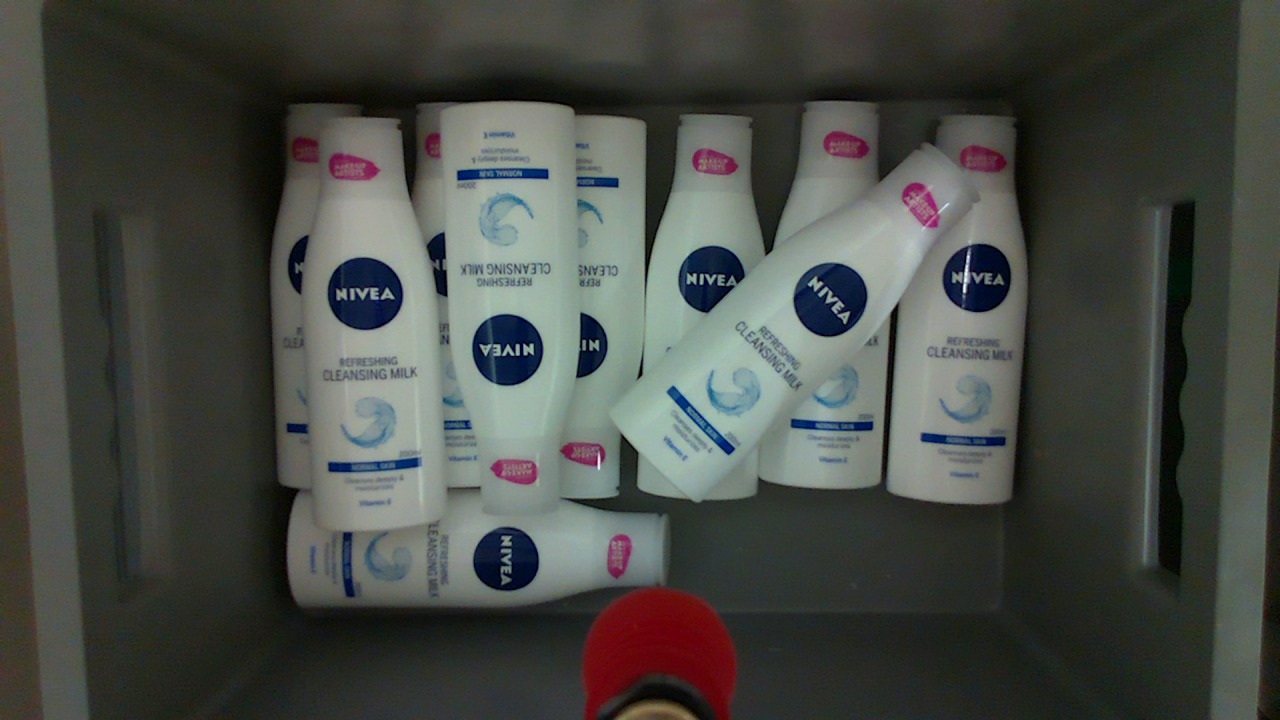
\includegraphics[width=0.37\textwidth]{graphics/results/0000.png}}
    %\hfill
    \hspace{2 cm}
    \subfloat{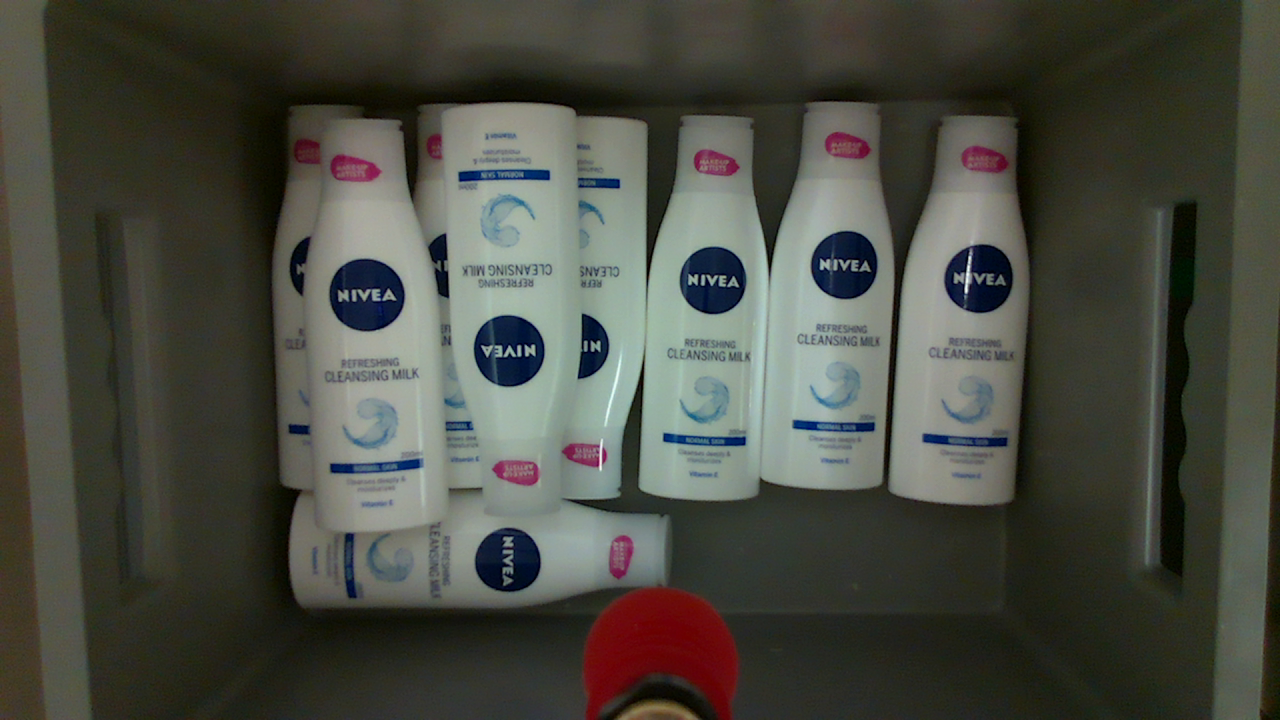
\includegraphics[width=0.37\textwidth]{graphics/results/0001.png}}
    %\hfill
    \hspace{2 cm}
    \subfloat{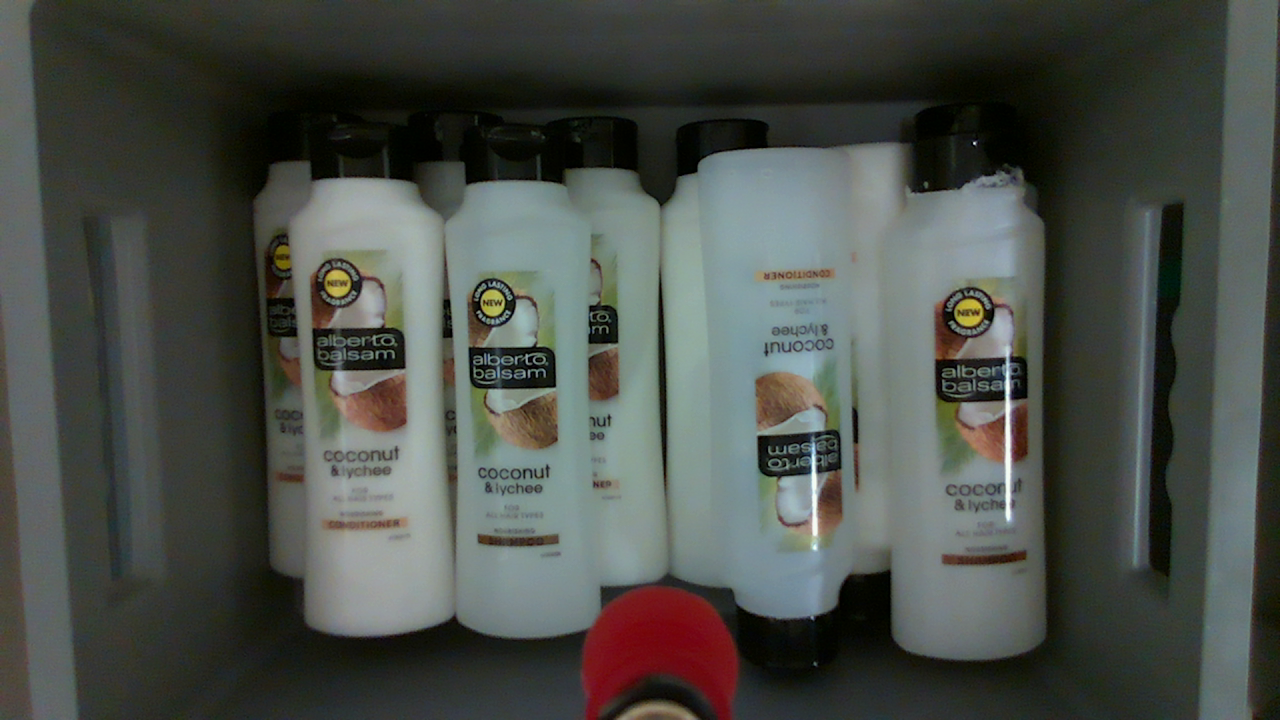
\includegraphics[width=0.37\textwidth]{graphics/results/0027.png}}
    %\hfill
    \hspace{2 cm}
    \subfloat{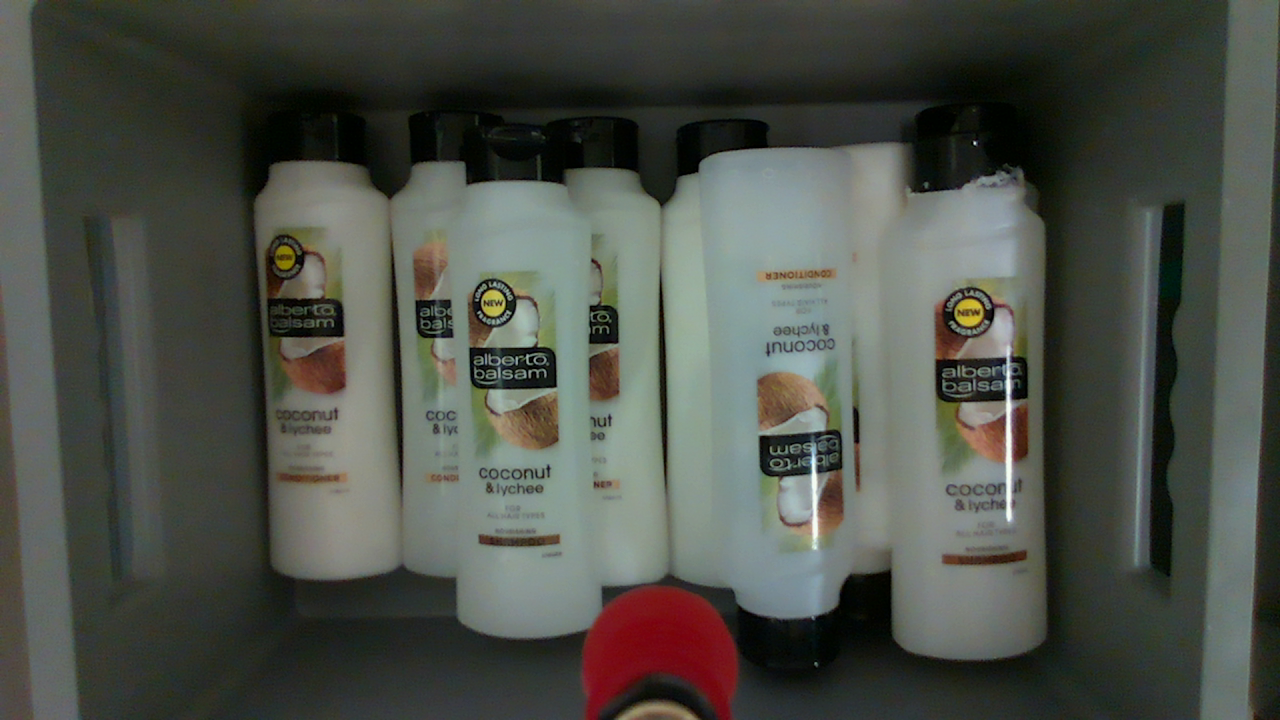
\includegraphics[width=0.37\textwidth]{graphics/results/0028.png}}
    \hspace{2 cm}
    \subfloat{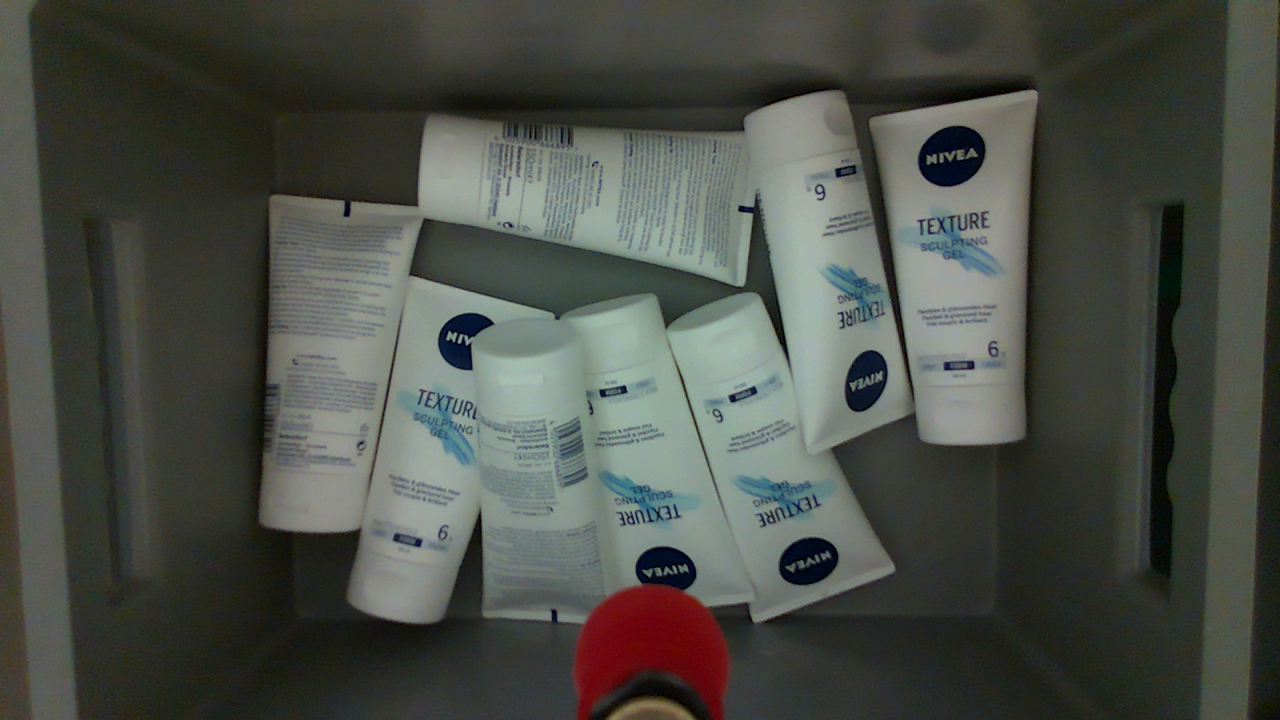
\includegraphics[width=0.37\textwidth]{graphics/results/0146.png}}
    %\hfill
    \hspace{2 cm}
    \subfloat{\includegraphics[width=0.37\textwidth]{graphics/results/0147.png}}
    \hspace{2 cm}
    \subfloat{\includegraphics[width=0.37\textwidth]{graphics/results/0075.png}}
    \hspace{2 cm}
    \subfloat{\includegraphics[width=0.37\textwidth]{graphics/results/0076.png}}
    %\hfill
    
    \caption{The second dataset contained 4 products with multiple objects in the bin}
    \label{figure: multiproducts}
\end{figure}

\subsection{Beiersdorf dataset}\label{sec:beiersdorfdataset}
A Beiersdorf dataset\cite{bjarnason_1984-_detecting_2021} was used in this project as a test dataset, it was created by a former master's student in Reykjavík University. 
The dataset consists of 15 products and included 145 images per item, up to total 2,175 images. This dataset was diverse, with similar items and also items that have different shapes. It should therefore provide a good indication of the expected performance of a trained model in a warehouse setting. \textit{Figure \ref{fig:beiersdorf}} shows the items that are in the dataset.

% \begin{figure}[h]
%     \centering
%     \includegraphics[width=1\textwidth]{graphics/methods/sverrirdataset.PNG}
%     \caption{Beiersdorf dataset contains 15 items\cite{bjarnason_1984-_detecting_2021}}
%     \label{fig:beiersdorf}
% \end{figure}

\begin{figure}[h]
    \centering
    % include first image
    \subfloat[Item 1]{\includegraphics[width=0.2\textwidth]{graphics/beiersdorf/i0001.png}}
    \hfill
    \subfloat[Item 2]{\includegraphics[width=0.2\textwidth]{graphics/beiersdorf/0155.png}}
    \hfill
    \subfloat[Item 3]{\includegraphics[width=0.2\textwidth]{graphics/beiersdorf/0300.png}}
    \hfill
    \subfloat[Item 4]{\includegraphics[width=0.2\textwidth]{graphics/beiersdorf/0450.png}}
    \hfill
    \subfloat[Item 5]{\includegraphics[width=0.2\textwidth]{graphics/beiersdorf/0650.png}}
    \hfill
    \subfloat[Item 6]{\includegraphics[width=0.2\textwidth]{graphics/beiersdorf/0750.png}}
    \hfill
    \subfloat[Item 7]{\includegraphics[width=0.2\textwidth]{graphics/beiersdorf/0950.png}}
    \hfill
    \subfloat[Item 8]{\includegraphics[width=0.2\textwidth]{graphics/beiersdorf/1050.png}}
    \hfill
    \subfloat[Item 9]{\includegraphics[width=0.2\textwidth]{graphics/beiersdorf/1250.png}}
    \hfill
    \subfloat[Item 10]{\includegraphics[width=0.2\textwidth]{graphics/beiersdorf/1350.png}}
    \hfill
    \subfloat[Item 11]{\includegraphics[width=0.2\textwidth]{graphics/beiersdorf/1470.png}}
    \hfill
    \subfloat[Item 12]{\includegraphics[width=0.2\textwidth]{graphics/beiersdorf/1650.png}}
    \hfill
    \subfloat[Item 13]{\includegraphics[width=0.2\textwidth]{graphics/beiersdorf/1750.png}}
    \hfill
    \subfloat[Item 14]{\includegraphics[width=0.2\textwidth]{graphics/beiersdorf/1950.png}}
    \hfill
    \subfloat[Item 15]{\includegraphics[width=0.2\textwidth]{graphics/beiersdorf/2050.png}}
    \caption{Beiersdorf dataset contains 15 items\cite{bjarnason_1984-_detecting_2021}}
    \label{fig:beiersdorf}
\end{figure}
The dataset includes manually annotated object masks in the form of polygons tracing the outline.  For use with Yolo, a bounding boxes were generated from the masks as the minimum and maximum vertex coordinate of each polygon.
It takes 2-10 minutes to annotate an image, averaging approximately 5 minutes per image. When the images are 2175 it takes around 181 hours to annotate all the images. Which is a lot of manpower for annotating images. \textit{Figure \ref{fig:beiersdorfanno}} shows how the dataset was annotated with a COCO annotator\cite{brooks_jsbrokscoco-annotator_2021}.
\begin{figure}[h]
    \centering
    \includegraphics[width=1\textwidth,  angle =0]{graphics/methods/sverrirannotated.PNG}
    \caption{Beiersdorf dataset annotated\cite{bjarnason_1984-_detecting_2021}}
    \label{fig:beiersdorfanno}
\end{figure}


%----------------
\section{Experiment setup}
A set of experiments were conducted with the aim to provide answers to the research questions.  In particular i) Is it possible to annotate objects automatically, determining the extent of the objects in the images? ii) Is it possible to generate new arrangements of objects using a robot manipulator? iii) Is it possible to improve the performance of a Convolutional Neural Network using automatically generated training data from robot? Those experiments will be explained in more detail in this section. 
\subsection{Robot performance}
In this experiment, one test was done on the Franka Emika robot and that was time performance over few iterations. In this particular test, there was only one object in the bin at a time. The time performance was tested on two items \textit{Alberto Balsam} and \textit{Nivea Cleansing Milk}, first with 100 iterations and then with 300 iterations. Which gave us the movement time for one object. In addition, it was checked if the robot needed some help to pick up the item. The robot code and how it works is explained in \textit{Section \ref{robotcontrol}}. 

\subsection{Automatic labelling performance}
The automatic labelling is not simple, since you need to look at few things such as lighting conditions, light reflection from objects, shades, etc. 
%So two methods were tested that were described in the methods chapter. 
In the automatic labeling experiment, two tests were performed on two methods that were mention in \textit{Sections \ref{beforeandafter}}

One test was performed on the \textit{Before vs After}. That test was simple and was only a visual inspection executed on the output images, to see how this method would affect the results.

The other test was performed on the \textit{Empty vs Item in the bin}. That test was executed by a visual inspection on the output images to check if the image has a good or bad annotations. An example of a good and bad annotation is shown in \textit{Figure \ref{figure: goodandbad}}. The time that it takes to annotate the images was also measured.

\begin{figure}[h]
    \centering
    \subfloat[Good annotation ]{\includegraphics[width=0.495\textwidth]{graphics/methods/albertobalsam100_0006box.png}}
    \hfill
    \subfloat[Bad annotation]{\includegraphics[width=0.495\textwidth]{graphics/methods/albertobalsam100_0050box.png}}
    \caption{An example of how good and bad annotations would look like}
    \label{figure: goodandbad}
\end{figure}
\vspace{1cm}

\subsection{Trained neural network performance}
\fxfatal{Describe here or refer to earlier description of the training setup, including network architecture (Yolov4), relevant sizes, image resolution, and implementation framework (with references).  Make special note of any relevant changes in hyper parameter values and refer to the config files in the appendix.}



\fxfatal{Nefna að ég hafi þjálfað netið tvisvar með sama data seti, einu sinni þar sem ég var búinn að eyða út vondum myndum og einu sinni þar sem þær voru inni !!!}
Three neural networks were trained from an automatically labeled datasets. 
First two neural networks uses almost the same dataset, but were trained on the automatically generated dataset with one object in the bin. But when training the first neural network bad annotations were removed from the dataset. 
So the difference between them are one is fully automatic and the other has human intervention on bad annotations.
The third neural network were trained on the automatically generated dataset with multiple objects in the bin.

When the neural networks had been trained three tests were done on the neural networks, IoU test, one visually, and an accuracy test(precision, recall, F1-score). These tests were made to see if the neural networks would improve. 

The first test was to measure which epochs model of the neural network would give us the best IoU on the test images. Epochs are the number of times the training set has been presented to the network.

The second test was done by comparing visually before and after results on the neural network, to find out if the trained neural network was better than the original network.

The third test was measuring the accuracy of object detection using a deep neural network trained on the robot-generated data. Measuring the IoU, recall, precision, and F-score and compare it to the results of manual labeling. 


\subsubsection{First neural network}
Before training the first neural network model using the automatically generated dataset with one object in the bin, it was split into a 75\% train dataset and 25\% test dataset. Images that had bad annotations were removed from the dataset. 


\subsubsection{Second neural network}
The second neural network was trained as the first neural network but, the difference was the second neural network was trained on all of the automatically generated dataset with one object in the bin. Before training the second neural network model using the automatically labeled dataset it was split into a 75\% train dataset and 25\% test dataset, which had both bad annotations and good annotations. 



\subsubsection{Third neural network}
The third neural network was trained on the automatically generated dataset with multiple objects in the bin. The automatically labeled dataset with multiple objects in the bin was split into a 75\% train dataset and 25\% test dataset before training the third neural network. %%RUM: "Methods"
%\part{The Second Part}
\chapter{Results}
% \textit{\ifdraft{In this section you discuss any issues that came up while developing
% the system. If you found something particularly interesting,
% difficult, or an important learning experience, put it here. This is
% also a good place to put additional figures and data.}}
The experimental results and evaluation of the proposed concept are covered in this chapter. Section \ref{resrobotcontrol} shows how the robot performed moving objects and creating new arrangements. Section \ref{rescamera} shows results from the automatically labelling. Section \ref{sec:resneural} shows results from the neural networks on images with objects in a bin. 

\section{Using a robot to create image data set}\label{resrobotcontrol}
%\textbf{Robot manipulator performance was measured by making tests on two products and measuring time, iterations, and interventions needed.} 
The performance of the Robot manipulator can be seen in \textit{Table \ref{tab:testonrobot}}, it has the item name, start position of the item in world-coordinates, how often the robot moved the object, how often the operator needed to interfere with the robot and help the robot to pick the object, time in seconds, whether the robot finished all the iterations without failing, how long it takes the robot to move one object and how often it needed intervention versus iterations. 


\vspace{1cm}
\begin{table}[h]
\caption{Test made on the robot and code performance.}
\resizebox{\textwidth}{!}{%
\begin{tabular}{clccccccc}
\hline
\textit{Test\#} &
 \textit{Item} &
 \textit{\begin{tabular}[c]{@{}c@{}}Start pos\\ {[}x, y, z{]}\end{tabular}} &
 \textit{Iterations} &
 \textit{\begin{tabular}[c]{@{}c@{}}Operator\\ intervention\end{tabular}} &
 \textit{\begin{tabular}[c]{@{}c@{}}Time \\ {[}sec{]}\end{tabular}} &
 \textit{\begin{tabular}[c]{@{}c@{}}Did it \\ finish?\end{tabular}} &
 \textit{\begin{tabular}[c]{@{}c@{}}Movement \\ time {[}sec{]}\end{tabular}} &
 \textit{\begin{tabular}[c]{@{}c@{}}Intervention\\ vs. Iterations\end{tabular}} \\ \hline
\multicolumn{1}{c|}{1} &
 \begin{tabular}[c]{@{}l@{}}Nivea \\ Cleansing Milk\end{tabular} &
 \begin{tabular}[c]{@{}c@{}}{[}0.336, \\ 0.045, \\ 0.097{]}\end{tabular} &
 100 &
 2 &
 1277.2 &
 Yes &
 12.77 &
 2.00\% \\
\multicolumn{1}{c|}{2} &
 \begin{tabular}[c]{@{}l@{}}Alberto \\ Balsam coconut\end{tabular} &
 \begin{tabular}[c]{@{}c@{}}{[}0.343, \\ 0.043, \\ 0.107{]}\end{tabular} &
 100 &
 0 &
 1254.2 &
 Yes &
 12.54 &
 0.00\% \\
\multicolumn{1}{c|}{3} &
 \begin{tabular}[c]{@{}l@{}}Nivea \\ Cleansing Milk\end{tabular} &
 \begin{tabular}[c]{@{}c@{}}{[}0.340 , \\ 0.044, \\ 0.098{]}\end{tabular} &
 300 &
 6 &
 3799.1 &
 Yes &
 12.66 &
 2.00\% \\
\multicolumn{1}{c|}{4} &
 \begin{tabular}[c]{@{}l@{}}Alberto \\ Balsam coconut\end{tabular} &
 \begin{tabular}[c]{@{}c@{}}{[}0.333 , \\ -0.040, \\ 0.118{]}\end{tabular} &
 300 &
 1 &
 3774.4&
 Yes &
 12.58 &
 0.33\% \\ \hline
\multicolumn{7}{r}{\textbf{Average:}} &
 12.64 &
 1.08\% \\ 
\end{tabular}%
}

\label{tab:testonrobot}
\end{table}
The most common intervention situations are when the robot would not pick the object, or some part of the robot end-effector crashed into the bin. To prevent that from happening the end effector was extended by 14 cm. The new extended end effector can be seen in the method chapter in \textit{Figure \ref{figure: newendeffector}}. When the robot end effector had been extended the robot worked every time without any operator intervention.
\clearpage
%%%%%%%%%%%%%%%%%%%%%%%%%%%%%%%%%%%%%%%%%%%%%%%%%%%%%%%%%%%%%%%%%%%%%
\section{Automatic labelling}\label{rescamera}
This section shows results from the automatically labelling for two different methods.

\subsection{Before vs. after}\label{subsec:beforeafter}
\begin{figure}[ht]
 \centering
 % include first image
 \subfloat[Before]{\includegraphics[width=0.35\textwidth]{graphics/results/tbefore.png}}
 \hspace{0.5cm}
 \subfloat[After]{\includegraphics[width=0.35\textwidth]{graphics/results/tafter.png}}
 \hspace{0.5cm}
 \subfloat[Contours]{\includegraphics[width=0.35\textwidth]{graphics/results/tmask1.png}}
 \hspace{0.5cm}
 \subfloat[Masked]{\includegraphics[width=0.35\textwidth]{graphics/results/tmasked.png}}
 \caption{Image Difference with OpenCV and Python, example of good annotation.}
 \label{figure: imagework1}
\end{figure}

\begin{figure}[ht]
 \centering
 % include first image
 \subfloat[Before]{\includegraphics[width=0.35\textwidth]{graphics/9before.png}}
 \hspace{0.5cm}
 \subfloat[After]{\includegraphics[width=0.35\textwidth]{graphics/9after.png}}
 \hspace{0.5cm}
 \subfloat[Contours]{\includegraphics[width=0.35\textwidth]{graphics/9filled.png}}
 \hspace{0.5cm}
 \subfloat[Masked]{\includegraphics[width=0.35\textwidth]{graphics/9masked.png}}
 \caption{Image Difference with OpenCV and Python, example of bad annotation.}
 \label{figure: imagework2}
\end{figure}

\textit{Figure \ref{figure: imagework1}} and \textit{Figure \ref{figure: imagework2}} show an example of good and bad automatic annotation. The figures show the items in before and after positions with only one object in the bin. In the bottom row the contoured difference and masked contour area can be seen. 
\clearpage
\begin{figure}[ht]
 \centering
 % include first image
 \subfloat[Before]{\includegraphics[width=0.4\textwidth]{graphics/results/newmulti-0019.png}}
 \hspace{0.5cm}
 \subfloat[After]{\includegraphics[width=0.4\textwidth]{graphics/results/newmulti-0020.png}}
 \hspace{0.5cm}
 \subfloat[Contours]{\includegraphics[width=0.4\textwidth]{graphics/results/newmulti-0019diff.png}}
 \hspace{0.5cm}
 \subfloat[Annotated]{\includegraphics[width=0.4\textwidth]{graphics/results/newmulti-0019marked.png}}
 \caption{Image Difference with OpenCV and Python, example of good annotation, with multiple objects in the bin.}
 \label{figure: multiimagework1}
\end{figure}

\begin{figure}[ht]
 \centering
 % include first image
 \subfloat[Before]{\includegraphics[width=0.4\textwidth]{graphics/results/newmulti-0051.png}}
 \hspace{0.5cm}
 \subfloat[After]{\includegraphics[width=0.4\textwidth]{graphics/results/newmulti-0052.png}}
 \hspace{0.5cm}
 \subfloat[Contours]{\includegraphics[width=0.4\textwidth]{graphics/results/newmulti-0051diff.png}}
 \hspace{0.5cm}
 \subfloat[Annotated]{\includegraphics[width=0.4\textwidth]{graphics/results/newmulti-0051marked.png}}
 \caption{Image Difference with OpenCV and Python, example of bad annotation, with multiple objects in the bin.}
 \label{figure: multiimagework2}
\end{figure}

\textit{Figure \ref{figure: multiimagework1}} and \textit{Figure \ref{figure: multiimagework2}} show an example of good and bad automatic annotation. The figures show an example of a before and after image when removing one object where there are multiple items in the bin. In the bottom row, the contoured difference and annotated object area can be seen. %The reason for bad annotation is because the two objects moved and not only one. 

\clearpage
\subsection{Empty bin vs. Object in the bin} \label{subsec:emptybin}
\begin{figure}[h]
 \centering
 % include first image
 \subfloat[Before annotation]{\includegraphics[width=0.37\textwidth]{graphics/results/9img3.png}}
 \hspace{0.5cm}
 \subfloat[Contours]{\includegraphics[width=0.37\textwidth]{graphics/results/9diff.png}}
 \hspace{0.5cm}
 \subfloat[Masked]{\includegraphics[width=0.37\textwidth]{graphics/results/9img1.png}}
 \hspace{0.5cm}
 \subfloat[After annotation]{\includegraphics[width=0.37\textwidth]{graphics/results/9img2.png}}
 \caption{An example of good annotation, from the empty bin vs. one item in the bin method.}
 \label{figure: labelling}
\end{figure}

\begin{figure}[h]
 \centering
 % include first image
 \subfloat
 [Before annotation]{\includegraphics[width=0.37\textwidth]{graphics/results/48img3.png}}
 \hspace{0.5cm}
 \subfloat[Contours]{\includegraphics[width=0.37\textwidth]{graphics/results/48diff.png}}
 \hspace{0.5cm}
 \subfloat[Masked]{\includegraphics[width=0.37\textwidth]{graphics/results/48img1.png}}
 \hspace{0.5cm}
 \subfloat[After annotation]{\includegraphics[width=0.37\textwidth]{graphics/results/48img2.png}}
 \caption{An example of bad annotation, from the empty bin vs. one item in the bin method.}
 \label{figure: badlabelling}
\end{figure}
%As can been seen in the \textit{Figure \ref{figure: labelling}} this method can be used to find the bounding box and to create a automatic labelled data. 
\textit{Figure \ref{figure: labelling}} and \textit{Figure \ref{figure: badlabelling}} show examples of successful and failed boundary box annotation, as determined by visual inspection. 

\clearpage

% Results from that test can been seen in \textit{Table \ref{tab:timediff}} and also it takes on average 0.85 second to label one image.

% Consider saying Figure 3.2 shows examples of successful and failed boundary box detection, as determined by visual inspection. A single example does not warrant stating that a method can be used. Leave this to the discussion, where you consider the results of the visual inspection. Consider adding more examples and a table with the number of successful and failed boundary box detections.



\begin{table}[h]
\caption{Measured time when using the difference.py.}
\resizebox{\textwidth}{!}{%
\begin{tabular}{clrrr}
\hline
\multicolumn{1}{l|}{\textit{Test \#}} &
 \textit{Item} &
 \multicolumn{1}{l}{\textit{Images}} &
 \multicolumn{1}{l}{\textit{Total time {[}s{]}}} &
 \multicolumn{1}{l}{\textit{Time per image {[}s{]}}} \\ \hline
\multicolumn{1}{c|}{1} & \begin{tabular}[c]{@{}l@{}}Nivea cleansing milk\end{tabular} & 300 & 255.99 & 0.85 \\
\multicolumn{1}{c|}{2} & \begin{tabular}[c]{@{}l@{}}Nivea cleansing milk\end{tabular} & 102 & 92.68 & 0.91 \\
\multicolumn{1}{c|}{3} & \begin{tabular}[c]{@{}l@{}}Nivea  elastic\end{tabular} & 72 & 56.31 & 0.78 \\
\multicolumn{1}{c|}{4} & \begin{tabular}[c]{@{}l@{}}Alberto Balsam coconut\end{tabular} & 102 & 88.30 & 0.87 \\ \hline
\multicolumn{4}{r}{\textbf{Average:}} & 0.85
\end{tabular}%
}

\label{tab:timediff}
\end{table}
A test was made on how long it would take to annotate one image. \textit{Table \ref{tab:timediff}} shows the results from that test. The average time to label one image is 0.85 seconds.

\begin{table}[h]
\caption{Annotation on the automatically generated dataset with one object in the bin.}
\resizebox{\textwidth}{!} \\ \hline
\multicolumn{1}{l|}{Alberto Balsam} & 101 & 95 & 6 & 5.9\% \\
\multicolumn{1}{l|}{Nivea Cleansing} & 102 & 102 & 0 & 0.0\% \\
\multicolumn{1}{l|}{Nivea Elastic} & 72 & 72 & 0 & 0.0\% \\
\multicolumn{1}{l|}{Nivea Texture} & 101 & 100 & 1 & 1.0\% \\ \hline
\multicolumn{4}{r}{\textbf{Average:}} & 1.9\%
\end{tabular}%
}
\label{tab:annotation}
\end{table}

In \textit{Table \ref{tab:annotation}} the annotation performance is shown where it can be seen that this method returned good annotation in 98.1\% cases on average. Six automatic labelled images did not have good annotation and they were images 34, 50, 71, 73, 83, and 93 of the Alberto Balsam. Bad annotation is when the bounding box does not frame the object tightly and is extremely bad when the center point is unsuitable for picking.



\clearpage
%%%%%%%%%%%%%%%%%%%%%%%%%%%%%%%%%%%%%%%%%%%%%%%%%%%%%%%%%%%%%%%%%%%%%
\section{Trained neural network}\label{sec:resneural}
This section shows how the neural networks performed on images with objects in a bin.

\subsection{Results from the first neural network} \label{sec:firstneural}
\begin{figure}[h]
 \centering
 \includegraphics[width=0.7\textwidth, trim={5cm 0 4cm 0},clip]{graphics/results/neuralnetworkauto.png}
 \caption{IoU is measured over the test set on the automatically generated dataset with one object in the bin, every 1000 epochs.}
 \label{fig:neuralnetwork}
\end{figure}
\textit{Figure \ref{fig:neuralnetwork}} shows how the IoU score developed over the number of epochs, when measuring over the test set. The best average IoU score can be seen in the red point and is 0.9584 at 38000 epochs. The average IoU is measured when running through the automatically generated dataset with one object in the bin (with only good annotations).

\begin{figure}[h]
 \centering
 % include first image
 \subfloat[The prior model]{\includegraphics[width=0.3\textwidth, trim={0 0.6cm 0 2cm},clip ]{graphics/results/beforetraining.png}}
 \hfill
 \subfloat[The prior model]{\includegraphics[width=0.3\textwidth, trim={0 0.6cm 0 2cm},clip]{graphics/results/beforetraining1.png}}
 \hfill
 \subfloat[The prior model]{\includegraphics[width=0.3\textwidth, trim={0 0.6cm 0 2cm},clip]{graphics/results/beforetraining2.png}}
 \hfill \newline
 \subfloat[The posterior model]{\includegraphics[width=0.3\textwidth, trim={0 0.6cm 0 2cm},clip]{graphics/results/aftertraining.png}}
 \hfill
 \subfloat[The posterior model]{\includegraphics[width=0.3\textwidth, trim={0 0.6cm 0 2cm},clip]{graphics/results/aftertraining1.png}}
 \hfill
 \subfloat[The posterior model]{\includegraphics[width=0.3\textwidth, trim={0 0.6cm 0 2cm},clip]{graphics/results/aftertraining2.png}}
 \caption{The prior model trained on the COCO dataset and the posterior model trained on the robot generated dataset by transfer learning, starting from the weights of the prior model.}
 \label{figure: beforeaftertraining}
\end{figure}
\textit{Figure \ref{figure: beforeaftertraining}} shows visually how the performance changed before and after training, images in top row shows the results from the prior model trained on the COCO dataset and images in the bottom row shows the results from the first neural network that was trained on these products.

\pagebreak
\subsubsection{Single known items}\label{sec:resontrained}
\begin{figure}[h]
 \centering
 % include first image
 \subfloat[Alberto Balsam]{\includegraphics[width=0.5\textwidth, trim={0.6cm 0 0.6cm 0},clip]{graphics/results/albertobalsamIOU.png}}
 \hfill
 \subfloat[Nivea Cleansing Milk]{\includegraphics[width=0.5\textwidth, trim={0.6cm 0 0.6cm 0},clip]{graphics/results/niveacleansingIOU.png}}
 \hfill
 \subfloat[Nivea Elastic]{\includegraphics[width=0.5\textwidth, trim={0.6cm 0 0.6cm 0},clip]{graphics/results/niveaelasticIOU.png}}
 \hfill
 \subfloat[Nivea Texture]{\includegraphics[width=0.5\textwidth, trim={0.6cm 0 0.6cm 0},clip]{graphics/results/niveatextureIOU.png}}
 \caption{Scatter plot for IoU on images of single items of known products.}
 \label{figure: knownproducts}
\end{figure}
\textit{Figure \ref{figure: knownproducts}} shows raw IoU data from detection run on the training and test set from the first dataset \textit{(Sec: \ref{sec:firstdataset})}, it also shows an average IoU line on each scatter plot.

\begin{table}[h]
\caption{Detection results when tested on the training and test set from the first dataset (\textit{Sec: \ref{sec:firstdataset}}) using the first neural network.}
\resizebox{\textwidth}{!}{% 
\begin{tabular}{l|rrrrrrrr}
\hline
\textit{Item} &
 \textit{Products} &
 \textit{Detections} &
 \textit{True Positive} &
 \textit{False Positive} &
 \textit{Avg-IoU} &
 \textit{Avg-Precision} &
 \textit{Avg-Recall} &
 \textit{Avg-F-score} \\ \hline
Alberto Balsam & 101 & 101 & 101 & 0 & 0.9468 & 1 & 1 & 1 \\
Nivea C. Milk & 102 & 102 & 102 & 0 & 0.9652 & 1 & 1 & 1 \\
Nivea Elastic & 101 & 101 & 101 & 0 & 0.9679 & 1 & 1 & 1 \\
Nivea Texture & 72 & 72 & 72 & 0 & 0.9620 & 1 & 1 & 1 \\ \hline
\multicolumn{5}{r}{\textbf{Average:}} & \textit{0.9605} & \textit{1} & \textit{1} & \textit{1} 
\end{tabular}%
}
\label{tab:ready}
\end{table}

\textit{Table \ref{tab:ready}} shows the results applying the model on the training and test set from the first dataset \textit{(Sec: \ref{sec:firstdataset})}. When using the first trained neural network on images of single items of known products.
\clearpage

\begin{figure}[h]
 \centering
 \includegraphics[width=0.8\textwidth]{graphics/results/boxplotForKnownProducts.png}
 \caption{Box plot for known products.}
 \label{fig:boxknownproducts}
\end{figure}

\textit{Figure \ref{fig:boxknownproducts}} shows the IoU on 4 known products in a box plot when there is only one item in the bin. The ends of the box are the upper and lower quartiles, the vertical line inside the box is the median, and the bottom line is a lower extremity and the top line is an upper extreme. The Alberto Balsam has 6 extreme outliers points, the reason for that is there were 6 automatic labelled images of Alberto Balsam that didn’t have good annotation. 


\begin{figure}[h]
 \centering
 \subfloat[Highest IoU score]{\includegraphics[width=0.5\textwidth]{graphics/results/v1Best.png}}
 \hfill
 \subfloat[Lowest IoU score]{\includegraphics[width=0.5\textwidth]{graphics/results/v1Worst.png}\label{figure: v1worst}}
 \caption{Highest and lowest IoU score on the first neural network.}
 \label{figure: v1bestworst}
\end{figure}

\textit{Figure \ref{figure: v1bestworst}} shows the highest and lowest IoU score on the first neural network when tested on the data set with one known item in the bin. The highest IoU score was 0.9973 and the lowest IoU score was 0.5494. The green bounding box is the automatically annotated bounding box and the red bounding box is created by the neural network. In the example with the lowest IoU score, it can be seen that the neural network created a better bounding box than the bounding box that was created by the automatic labelling process.

\clearpage
\subsubsection{On unknown Beiersdorf products}\label{subsec:resunknownprod}
\begin{figure}[h]
 \centering
 % include first image
 \subfloat[Item 11]{\includegraphics[width=0.5\textwidth, trim={0.6cm 0 0.6cm 0},clip]{graphics/results/item11.png}}
 \hfill
 % \subfloat[Item 12]{\includegraphics[width=0.245\textwidth]{graphics/results/item12.png}}
 % \hfill
 % \subfloat[Item 5]{\includegraphics[width=0.245\textwidth]{graphics/results/item5.png}}
 % \hfill
 \subfloat[Item 6]{\includegraphics[width=0.5\textwidth, trim={0.6cm 0 0.6cm 0},clip]{graphics/results/item6.png}}
 \caption{Scatter plot for IoU on images of multiple items of unknown products.}
 \label{figure: unknownproducts}
\end{figure}

\textit{Figure \ref{figure: unknownproducts}} shows raw IoU data from detection run on the Beiersdorf dataset \textit{(Sec: \ref{sec:beiersdorfdataset})}, it also shows an average IoU line on each scatter plot. The Beiersdorf data set has multiple unknown objects in the bin in each image.
Item nr. 11 had the highest average IoU or 0.7548 and item nr. 6 had the lowest average IoU or 0.2944. Raw data can be seen in the \textit{Appendix \ref{sec:apIoUresults}}.
% Please add the following required packages to your document preamble:
% \usepackage{graphicx}
\begin{table}[h]
\caption{The results when tested on unknown data, using the first neural network.}
\resizebox{\textwidth}{!}{%
\begin{tabular}{rrrrrrrrr}
\hline
\multicolumn{1}{c|}{\textit{Item}} & \textit{Products} & \textit{Detections} & \textit{True Positive} & \textit{False Positive} & \textit{Avg-IoU} & \textit{Avg-Precision} & \textit{Avg-Recall} & \textit{Avg-F-score} \\ \hline
\multicolumn{1}{c|}{1} & 684 & 361 & 334 & 24 & 0.6899 & 0.8540 & 0.5479 & 0.6373 \\
\multicolumn{1}{c|}{2} & 1029 & 443 & 385 & 58 & 0.6123 & 0.7729 & 0.4340 & 0.5231 \\
\multicolumn{1}{c|}{3} & 667 & 412 & 382 & 30 & 0.7145 & 0.8770 & 0.6299 & 0.7087 \\
\multicolumn{1}{c|}{4} & 683 & 412 & 387 & 24 & 0.7246 & 0.8992 & 0.6260 & 0.7068 \\
\multicolumn{1}{c|}{5} & 892 & 381 & 291 & 90 & 0.4940 & 0.6533 & 0.3397 & 0.4317 \\
\multicolumn{1}{c|}{6} & 918 & 225 & 93 & 129 & 0.2944 & 0.2862 & 0.1150 & 0.1588 \\
\multicolumn{1}{c|}{7} & 851 & 415 & 344 & 71 & 0.6008 & 0.7613 & 0.4117 & 0.5207 \\
\multicolumn{1}{c|}{8} & 788 & 362 & 339 & 23 & 0.7023 & 0.9182 & 0.4631 & 0.5893 \\
\multicolumn{1}{c|}{9} & 887 & 360 & 294 & 66 & 0.5417 & 0.7176 & 0.3551 & 0.4600 \\
\multicolumn{1}{c|}{10} & 665 & 370 & 332 & 38 & 0.6625 & 0.8184 & 0.5293 & 0.6229 \\
\multicolumn{1}{c|}{11} & 627 & 407 & 386 & 21 & 0.7548 & 0.9264 & 0.6628 & 0.7500 \\
\multicolumn{1}{c|}{12} & 574 & 453 & 431 & 20 & 0.7428 & 0.9380 & 0.7891 & 0.8349 \\
\multicolumn{1}{c|}{13} & 618 & 329 & 320 & 9 & 0.7450 & 0.9552 & 0.5786 & 0.6891 \\
\multicolumn{1}{c|}{14} & 1031 & 312 & 230 & 70 & 0.4798 & 0.6666 & 0.2746 & 0.3609 \\
\multicolumn{1}{c|}{15} & 616 & 330 & 310 & 18 & 0.7272 & 0.9040 & 0.5607 & 0.6602 \\ \hline
\multicolumn{5}{r}{\textbf{Average:}} &\textit{ 0.6324} & \textit{0.7966} & \textit{0.4878} & \textit{0.5770}
\end{tabular}%
}
\label{tab:test1unknown}
\end{table}

\textit{Table \ref{tab:test1unknown}} shows the results from the detection run on the Beiersdorf dataset \textit{(Sec: \ref{sec:beiersdorfdataset})} when using the trained first neural network on unknown products. As can be seen item nr. 12 has the best average precision, recall, and F-score.

% \begin{figure}[h]
% \centering
% \includegraphics[width=1\textwidth, trim={8cm 0 8cm 0},clip]{graphics/results/boxplotForProducts.png}
% \caption{Box plot for unknown products, Intersection over Union on the left and F-score on the right}
% \label{fig:boxunknownproducts}
% \end{figure}
\clearpage

\begin{figure}[h]
 \centering
 % include first image
 \subfloat[Intersection over Union]{\includegraphics[width=0.5\textwidth, trim={0.5cm 0 1.5cm 0},clip]{graphics/results/iouboxplotForProducts.png}\label{fig:unknownioua}}
 \hfill
 \subfloat[F-score]{\includegraphics[width=0.5\textwidth, trim={0.5cm 0 1.5cm 0},clip]{graphics/results/f1boxplotForProducts.png}\label{fig:unknownioub}}
 
 \caption{Box plot on results for unknown products.}
 \label{fig:unknowniou}
\end{figure}

\textit{Figure \ref{fig:unknowniou}} shows the IoU and F-score on 15 unknown products in a box plot when using the first neural network.
\begin{figure}[h]
 \centering
 \includegraphics[width=0.9\textwidth]{graphics/results/boxplotBottles.png}
 \caption{IoU box plot for different number of items in the bin.}
 \label{fig:bottles}
\end{figure}

\textit{Figure \ref{fig:bottles}} shows also the IoU in the box plot, but for a different number of objects in the bin when using the first neural network. In this box plot, the X-axis is the number of bottles in the bin. The IoU has the highest IoU for single items and trends towards lower values as the number of items in the bin increases.
% You can point out to the reader that the IoU is highest for single items and trends towards lower values as the number of items in the bin increases. This is the plot to beat in the next experiment :-)]

\begin{figure}[h]
 \centering
 % include first image
 \subfloat[Highest IoU score, item nr. 11 ]{\includegraphics[width=0.5\textwidth]{graphics/results/v1best1.png}\label{fig:unknowniouaa}}
 \hfill
 \subfloat[Lowest IoU score, item nr. 6 ]{\includegraphics[width=0.5\textwidth]{graphics/results/v1worst1.png}\label{fig:unknownioubb}}
 
 \caption{Highest and lowest IoU score on the first neural network when testing on unknown items.}
 \label{fig:v1unknowniou}
\end{figure}
\textit{Figure \ref{fig:v1unknowniou}} shows the highest and the lowest IoU score when using the first neural network on the Beiersdorf dataset, it can be seen that the highest IoU score is 0.9763 on item nr. 11 and the lowest IoU score is 0.00 on item nr 6.

\begin{figure}[h]
 \centering
 % include first image
 \subfloat[Highest True Positive detection, item nr. 9 ]{\includegraphics[width=0.5\textwidth]{graphics/results/ioumaxtrue.png}\label{fig:v1maxtrue}}
 \hfill
 \subfloat[Highest False Positive detection, item nr. 5 ]{\includegraphics[width=0.5\textwidth]{graphics/results/ioumaxfalse.png}\label{fig:v1maxfalse}}
 
 \caption{Highest True and False Positive detection using the first neural network on unknown items.}
 \label{fig:v1max}
\end{figure}
\textit{Figure \ref{fig:v1max}} shows the highest True Positive (TP) detection and the highest False Positive (FP) detection when using the first neural network on the Beiersdorf dataset, it can be seen that the highest TP is 7 objects and the highest FP is 4 objects.
\clearpage

\subsection{Results from the second neural network}\label{sec:secondneural}

\begin{figure}[h]
 \centering
 \includegraphics[width=0.8\textwidth, trim={5cm 0 4cm 0},clip]{graphics/results/secondneuralnetworkauto.png}
 \caption{IoU is measured over the test set on the automatically generated dataset with one object in the bin, every 1000 epochs.}
 \label{fig:v2neuralnetwork}
\end{figure}
\textit{Figure \ref{fig:v2neuralnetwork}} shows how the IoU score developed over the number of epochs, when measuring over the test set. The best average IoU score can be seen in the red point and is 0.9546 at 37000 epochs. The average IoU is measured when running through the automatically generated dataset with one object in the bin (with both good and bad annotations).

%\fxfatal{skrifa meira setja inn mynd af því hvernig netið hegðar sér visually í bin eins og fyrsta neural}

\begin{figure}[h]
 \centering
 % include first image
 \subfloat[The prior model]{\includegraphics[width=0.33\textwidth, trim={0 0.6cm 0 2cm},clip ]{graphics/results/fullbinyolo-balsam.png}}
 \hfill
 \subfloat[The prior model]{\includegraphics[width=0.33\textwidth, trim={0 0.6cm 0 2cm},clip]{graphics/results/fullbinyolo-clean.png}}
 \hfill
 \subfloat[The prior model]{\includegraphics[width=0.33\textwidth, trim={0 0.6cm 0 2cm},clip]{graphics/results/fullbinyolo-elastic.png}}
 \hfill \newline
 \subfloat[The posterior model]{\includegraphics[width=0.33\textwidth, trim={0 0.6cm 0 2cm},clip]{graphics/results/fullbinv2-balsam.png}}
 \hfill
 \subfloat[The posterior model]{\includegraphics[width=0.33\textwidth, trim={0 0.6cm 0 2cm},clip]{graphics/results/fullbinv2-clean.png}}
 \hfill
 \subfloat[The posterior model]{\includegraphics[width=0.3\textwidth, trim={0 0.6cm 0 2cm},clip]{graphics/results/fullbinv2-elastic.png}}
 \caption{The prior model trained on the COCO dataset and the posterior model trained on the robot generated dataset by transfer learning, starting from the weights of the prior model.}
 \label{figure: v2beforeaftertraining}
\end{figure}
\textit{Figure \ref{figure: v2beforeaftertraining}} shows visually how the performance changed before and after training on bin full of objects, images in top row show the results from the prior model trained on the COCO dataset and images in the bottom row show the results from the second neural network that was trained on these products.

\clearpage
\subsubsection{Single known items} \label{sec:v2resontrained}
\begin{figure}[h]
 \centering
 % include first image
 \subfloat[Alberto Balsam]{\includegraphics[width=0.5\textwidth, trim={0.6cm 0 0.6cm 0},clip]{graphics/results/v2albertobalsamIOU.png}}
 \hfill
 \subfloat[Nivea Cleansing Milk]{\includegraphics[width=0.5\textwidth, trim={0.6cm 0 0.6cm 0},clip]{graphics/results/v2niveacleansingIOU.png}}
 \hfill
 \subfloat[Nivea Elastic]{\includegraphics[width=0.5\textwidth, trim={0.6cm 0 0.6cm 0},clip]{graphics/results/v2niveaelasticIOU.png}}
 \hfill
 \subfloat[Nivea Texture]{\includegraphics[width=0.5\textwidth, trim={0.6cm 0 0.6cm 0},clip]{graphics/results/v2niveatextureIOU.png}}
 \caption{Scatter plot for IoU on images of single items of known products.} %Scatter plot for IoU on images of multiple items of unknown products
 \label{figure: v2knownproducts}
\end{figure}
\textit{Figure \ref{figure: v2knownproducts}} shows raw IoU data from detection run on the training and test set from the first dataset \textit{(Sec: \ref{sec:firstdataset})}, it also shows an average IoU line on each scatter plot.

\begin{table}[h]
\caption{Detection results when tested on trained data using the second neural network.}
\resizebox{\textwidth}{!}{% 
\begin{tabular}{l|rrrrrrrrr}
\hline
\textit{Item} &
 \textit{Products} &
 \textit{Detections} &
 \textit{True Positive} &
 \textit{False Positive} &
 \textit{Avg-IoU} &
 \textit{Avg-Precision} &
 \textit{Avg-Recall} &
 \textit{Avg-F-score} \\ \hline
Alberto Balsam & 101 & 101 & 101 & 0 & 0.9512 & 1 & 1 & 1 \\
Nivea C. Milk & 102 & 102 & 102 & 0 & 0.9627 & 1 & 1 & 1 \\
Nivea Elastic & 101 & 101 & 101 & 0 & 0.9635 & 1 & 1 & 1 \\
Nivea Texture & 72 & 72 & 72 & 0 & 0.9575 & 1 & 1 & 1 \\ \hline
\multicolumn{5}{r}{\textbf{Average:}} & \textit{0.9587} & \textit{1} & \textit{1} & \textit{1} 
\end{tabular}%
}
\label{tab:v2ready}
\end{table}
\textit{Table \ref{tab:v2ready}} shows the results from the detection run on the first dataset \textit{(Sec: \ref{sec:firstdataset})} when using the second trained neural network on images of single items of known products.

\clearpage
\begin{figure}[h]
 \centering
 \includegraphics[width=0.8\textwidth]{graphics/results/v2boxplotForKnownProducts.png}
 \caption{Box plot for known products.}
 \label{fig:v2boxknownproducts}
\end{figure}
\textit{Figure \ref{fig:v2boxknownproducts}} shows the IoU on 4 known products in a box plot when there is only one item in the bin. The ends of the box are the upper and lower quartiles, the vertical line inside the box is the median, and the bottom line is a lower extremity, and the top line is an upper extreme. The Alberto Balsam has 4 extreme outlier’s points, the reason for that is there were 6 automatic labelled images of Alberto Balsam that didn’t have good annotation. 

\begin{figure}[h]
 \centering
 \subfloat[Highest IoU score]{\includegraphics[width=0.5\textwidth]{graphics/results/v2Best.png}}
 \hfill
 \subfloat[Lowest IoU score]{\includegraphics[width=0.5\textwidth]{graphics/results/v2Worst.png}}
 \caption{Highest and lowest IoU score on the second neural network.}
 \label{figure: v2bestworst}
\end{figure}

\textit{Figure \ref{figure: v2bestworst}} shows the highest and lowest IoU score on the second neural network when tested on the data set with one known item in the bin. The highest IoU score was 0.9974 and the lowest IoU score was 0.6730. The green bounding box is the automatically annotated bounding box and the red bounding box is the bounding box created by the second neural network.

\clearpage
\subsubsection{On unknown Beiersdorf products}\label{subsec:v2resunknownprod}

\begin{figure}[h]
 \centering
 % include first image
 \subfloat[Item 11]{\includegraphics[width=0.5\textwidth, trim={0.6cm 0 0.6cm 0},clip]{graphics/results/v2item11.png}}
 \hfill
 % \subfloat[Item 12]{\includegraphics[width=0.245\textwidth]{graphics/results/item12.png}}
 % \hfill
 % \subfloat[Item 5]{\includegraphics[width=0.245\textwidth]{graphics/results/item5.png}}
 % \hfill
 \subfloat[Item 6]{\includegraphics[width=0.5\textwidth, trim={0.6cm 0 0.6cm 0},clip]{graphics/results/v2item6.png}}
 \caption{Scatter plot for IoU on images of multiple items of unknown products.}
 \label{figure: v2unknownproducts}
\end{figure}

\textit{Figure \ref{figure: v2unknownproducts}} shows raw IoU data from detection run on the Beiersdorf dataset \textit{(Sec: \ref{sec:beiersdorfdataset})}, it also shows an average IoU line on each scatter plot. The Beiersdorf data set has multiple items of unknown objects in the bin in each image.
Item nr. 11 had the highest average IoU or 0.7549 and item nr. 6 had the lowest average IoU or 0.2456. 

% Please add the following required packages to your document preamble:
% \usepackage{graphicx}
% Please add the following required packages to your document preamble:
% \usepackage{graphicx}
\begin{table}[h]
\caption{The results when tested on unknown data, using the second neural network.}
\resizebox{\textwidth}{!}{%
\begin{tabular}{c|rrrrrrrr}
\hline
\textit{Item} &
 \textit{Products} &
 \textit{Detections} &
 \textit{True Positive} &
 \textit{False Positive} &
 \textit{Avg-IoU} &
 \textit{Avg-Precision} &
 \textit{Avg-Recall} &
 \textit{Avg-F-score} \\ \hline
1 & 684 & 375 & 359 & 16 & 0.7106 & 0.9090 & 0.5840 & 0.6806 \\
2 & 1029 & 481 & 417 & 64 & 0.6008 & 0.7789 & 0.4641 & 0.5521 \\
3 & 667 & 413 & 385 & 28 & 0.7035 & 0.8810 & 0.6316 & 0.7135 \\
4 & 683 & 436 & 415 & 21 & 0.7272 & 0.9220 & 0.6599 & 0.7368 \\
5 & 892 & 262 & 175 & 87 & 0.4454 & 0.5408 & 0.2092 & 0.2891 \\
6 & 918 & 174 & 45 & 129 & 0.2456 & 0.1678 & 0.0563 & 0.0814 \\
7 & 851 & 381 & 297 & 84 & 0.5894 & 0.7090 & 0.3575 & 0.4622 \\
8 & 788 & 400 & 374 & 26 & 0.6932 & 0.9040 & 0.5070 & 0.6284 \\
9 & 887 & 369 & 299 & 70 & 0.5326 & 0.7082 & 0.3670 & 0.4675 \\
10 & 665 & 386 & 355 & 31 & 0.6802 & 0.8552 & 0.5609 & 0.6577 \\
11 & 627 & 432 & 407 & 25 & 0.7549 & 0.9159 & 0.6920 & 0.7679 \\
12 & 574 & 451 & 437 & 14 & 0.7490 & 0.9582 & 0.7963 & 0.8481 \\
13 & 618 & 345 & 335 & 10 & 0.7314 & 0.9408 & 0.5938 & 0.6978 \\
14 & 1031 & 291 & 243 & 48 & 0.5510 & 0.7210 & 0.2878 & 0.3823 \\
15 & 616 & 333 & 315 & 18 & 0.7348 & 0.8943 & 0.5603 & 0.6584 \\ \hline
\textit{\textbf{Average:}} &
 \textit{\textbf{769}} &
 \textit{\textbf{369}} &
 \textit{\textbf{324}} &
 \textit{\textbf{45}} &
 \textit{\textbf{0.6300}} &
 \textit{\textbf{0.7871}} &
 \textit{\textbf{0.4885}} &
 \textit{\textbf{0.5749}} \\ \hline
\textit{\textbf{Total:}} &
 \textit{\textbf{11530}} &
 \textit{\textbf{5529}} &
 \textit{\textbf{4858}} &
 \textit{\textbf{671}} &
 \textbf{-} &
 \textbf{-} &
 \textbf{-} &
 \textbf{-} \\ \hline
\end{tabular}%
}
\label{tab:test2unknown}
\end{table}
\textit{Table \ref{tab:test2unknown}} shows the results from the detection run on the Beiersdorf dataset \textit{(Sec: \ref{sec:beiersdorfdataset})} when using the trained second neural network on unknown products. As can be seen item nr. 12 has the best average precision, recall, and F-score.


\clearpage

\begin{figure}[h]
 \centering
 % include first image
 \subfloat[Intersection over Union]{\includegraphics[width=0.5\textwidth, trim={0.5cm 0 1.5cm 0},clip]{graphics/results/v2iouboxplotForProducts.png}\label{fig:v2unknownioua}}
 \hfill
 \subfloat[F-score]{\includegraphics[width=0.5\textwidth, trim={0.5cm 0 1.5cm 0},clip]{graphics/results/v2f1boxplotForProducts.png}\label{fig:v2unknownioub}}
 
 \caption{Box plot on results for unknown products.}
 \label{fig:v2unknowniou}
\end{figure}

\textit{Figure \ref{fig:v2unknowniou}} shows the IoU and F-score on 15 unknown products in a box plot when using the second neural network.

\begin{figure}[h]
 \centering
 \includegraphics[width=0.8\textwidth]{graphics/results/v2boxplotBottles.png}
 \caption{IoU box plot for different number of items in the bin.}
 \label{fig:v2bottles}
\end{figure}

\textit{Figure \ref{fig:v2bottles}} shows also the IoU in the box plot, but for a different number of objects in the bin when using the second neural network. In this box plot, the X-axis is the number of bottles in the bin. The IoU has the highest IoU for single items and trends towards lower values as the number of items in the bin increases.

\clearpage
\begin{figure}[h]
 \centering
 % include first image
 \subfloat[Highest IoU score, item nr. 13 ]{\includegraphics[width=0.5\textwidth]{graphics/results/v2best1.png}\label{fig:v2unknowniouaa}}
 \hfill
 \subfloat[Lowest IoU score, item nr. 5]{\includegraphics[width=0.5\textwidth]{graphics/results/v2worst1.png}\label{fig:v2unknownioubb}}
 
 \caption{Highest and lowest IoU score on the second neural network when testing on unknown items.}
 \label{fig:v2unknowniou2}
\end{figure}

\textit{Figure \ref{fig:v2unknowniou2}} shows the highest and the lowest IoU score when using the second neural network on the Beiersdorf dataset, it can be seen that the highest IoU score is 0.9862 on item nr. 13 and the lowest IoU score is 0.00 on item nr. 5.

\begin{figure}[h]
 \centering
 % include first image
 \subfloat[Highest True positive detection, item nr. 2 ]{\includegraphics[width=0.5\textwidth]{graphics/results/v2ioumaxtrue.png}\label{fig:v2maxtrue}}
 \hfill
 \subfloat[Highest False Positive detection, item nr. 9 ]{\includegraphics[width=0.5\textwidth]{graphics/results/v2ioumaxfalse.png}\label{fig:v2maxfalse}}
 
 \caption{Highest True and False Positive detection using the second neural network on unknown items.}
 \label{fig:v2max}
\end{figure}

\textit{Figure \ref{fig:v2max}} shows the highest True Positive (TP) detection and the highest False Positive (FP) detection when using the second neural network on the Beiersdorf dataset, it can be seen that the highest TP is 7 objects and the highest FP is 4 objects.

\clearpage
\subsubsection{On unknown Beiersdorf products - one detection per image}\label{subsec:v2zero}
Since the neural network is trained on images with only one annotation per image, the data was changed so it would be possible to see how it performs finding just one item per image.
% Please add the following required packages to your document preamble:
% \usepackage{graphicx}
\begin{table}[h]
\caption{The results when tested on unknown data, and assuming one detection per each image.}
\resizebox{\textwidth}{!}{%
\begin{tabular}{c|rrrrrrrr}
\hline
\textit{Item} &
 \textit{Products} &
 \textit{Detections} &
 \textit{True Positive} &
 \textit{False Positive} &
 \textit{Avg-IoU} &
 \textit{Avg-Precision} &
 \textit{Avg-Recall} &
 \textit{Avg-F-score} \\ \hline
1 & 145 & 142 & 136 & 6 & 0.7256 & 0.9379 & 0.9379 & 0.9379 \\
2 & 145 & 145 & 126 & 19 & 0.6008 & 0.8690 & 0.8690 & 0.8690 \\
3 & 145 & 145 & 135 & 10 & 0.7035 & 0.9310 & 0.9310 & 0.9310 \\
4 & 145 & 145 & 140 & 5 & 0.7272 & 0.9655 & 0.9655 & 0.9655 \\
5 & 145 & 136 & 94 & 42 & 0.4749 & 0.6483 & 0.6483 & 0.6483 \\
6 & 145 & 135 & 37 & 98 & 0.2638 & 0.2552 & 0.2552 & 0.2552 \\
7 & 145 & 145 & 131 & 14 & 0.5894 & 0.9034 & 0.9034 & 0.9034 \\
8 & 145 & 145 & 140 & 5 & 0.6932 & 0.9655 & 0.9655 & 0.9655 \\
9 & 145 & 144 & 116 & 28 & 0.5363 & 0.8000 & 0.8138 & 0.8138 \\
10 & 145 & 145 & 131 & 14 & 0.6802 & 0.9034 & 0.9034 & 0.9034 \\
11 & 145 & 145 & 141 & 4 & 0.7549 & 0.9724 & 0.9724 & 0.9724 \\
12 & 145 & 144 & 143 & 1 & 0.7542 & 0.9862 & 0.9862 & 0.9862 \\
13 & 145 & 144 & 138 & 6 & 0.7365 & 0.9517 & 0.9517 & 0.9517 \\
14 & 145 & 135 & 113 & 22 & 0.5918 & 0.7793 & 0.7793 & 0.7793 \\
15 & 145 & 141 & 134 & 7 & 0.7556 & 0.9241 & 0.9241 & 0.9241 \\ \hline
\textit{\textbf{Average:}} &
 \textit{\textbf{145}} &
 \textit{\textbf{142}} &
 \textit{\textbf{124}} &
 \textit{\textbf{19}} &
 \textit{\textbf{0.6392}} &
 \textit{\textbf{0.8529}} &
 \textit{\textbf{0.8538}} &
 \textit{\textbf{0.8538}} \\ \hline
\textit{\textbf{Total:}} &
 \textit{\textbf{2175}} &
 \textit{\textbf{2136}} &
 \textit{\textbf{1855}} &
 \textit{\textbf{281}} &
 \textbf{-} &
 \textbf{-} &
 \textbf{-} &
 \textbf{-} \\ \hline
\end{tabular}%
}
\label{tab:v2zero}
\end{table}
%

\textit{Table \ref{tab:v2zero}} shows the results from the detection run on the Beiersdorf dataset \textit{(Sec: \ref{sec:beiersdorfdataset})} when using the trained second neural network on unknown products, but images with zero detections are not used to calculate the IoU. %As can be seen item nr. 15 has the best average IoU and precision, but item nr. 12 has the best recall and F1.

\begin{figure}[h]
 \centering
 % include first image
 \subfloat[Intersection over Union]{\includegraphics[width=0.5\textwidth, trim={0.5cm 0 1.5cm 0},clip]{graphics/v2zeroioubox.png}\label{fig:v2zeroa}}
 \hfill
 % \subfloat[F-score]{\includegraphics[width=0.33\textwidth, trim={0.5cm 0 1.5cm 0},clip]{graphics/v2zerof1box.png}\label{fig:v2zerob}}
 % \hfill
 \subfloat[Intersection over Union for different number of items in the bin]{\includegraphics[width=0.5\textwidth, trim={0.5cm 0 1.5cm 0},clip]{graphics/v2zerobottles.png}\label{fig:v2zeroc}}
 
 \caption{Box plot on results for unknown products, when zero detections are eliminated.}
 \label{fig:v2zerofig}
\end{figure}

\textit{Figure \ref{fig:v2zerofig}} shows the IoU and the IoU for a different number of items in the bin, on 15 unknown products in a box plot when using the second neural network.


\clearpage
%%%%%%%%%%%%%%%%%%%%%%% Third neural network ------------------
\subsection{Results from the third neural network}
\begin{figure}[h]
 \centering
 \includegraphics[width=0.8\textwidth, trim={5cm 0 4cm 0},clip]{graphics/results/thirdneuralnetwork.png}
 \caption{IoU is measured over the test set on the automatically generated dataset with multiple objects in the bin, every 1000 epochs.}
 \label{fig:v3neuralnetwork}
\end{figure}
\textit{Figure \ref{fig:v3neuralnetwork}} shows how the IoU score developed over the number of epochs when measuring over the test set. The best average IoU score on the test set can be seen in the red point and is 0.9067 at 22000 epochs. The average IoU is measured when running through the automatically generated dataset with multiple objects in the bin.

%\fxfatal{Skrifa þegar ég fæ result ur þvi}

\begin{figure}[h]
 \centering
 % include first image
 \subfloat[Second neural network]{\includegraphics[width=0.33\textwidth, trim={0 0.6cm 0 2cm},clip ]{graphics/results/v2-1.png}}
 \hfill
 \subfloat[Second neural network]{\includegraphics[width=0.33\textwidth, trim={0 0.6cm 0 2cm},clip]{graphics/results/v2-2.png}}
 \hfill
 \subfloat[Second neural network]{\includegraphics[width=0.33\textwidth, trim={0 0.6cm 0 2cm},clip]{graphics/results/v2-3.png}}
 \hfill \newline
 \subfloat[Third neural network]{\includegraphics[width=0.33\textwidth, trim={0 0.6cm 0 2cm},clip]{graphics/results/v3-1.png}}
 \hfill
 \subfloat[Third neural network]{\includegraphics[width=0.33\textwidth, trim={0 0.6cm 0 2cm},clip]{graphics/results/v3-2.png}}
 \hfill
 \subfloat[Third neural network]{\includegraphics[width=0.33\textwidth, trim={0 0.6cm 0 2cm},clip]{graphics/results/v3-3.png}}
 \caption{Performance using the second neural network and third neural network.}
 \label{figure: v3beforeaftertraining}
\end{figure}
\textit{Figure \ref{figure: v3beforeaftertraining}} shows visually how the performance changed from the second neural network (\textit{trained on automatically generated dataset with one object in the bin}) and third neural network (\textit{trained on automatically generated dataset with multiple objects in the bin}). 
\clearpage
\subsubsection{On multiple known items} \label{sec:v3resontrained}
\begin{figure}[h]
 \centering
 % include first image
 \subfloat[Alberto Balsam]{\includegraphics[width=0.5\textwidth, trim={0.6cm 0 0.6cm 0},clip]{graphics/results/v3albertobalsamIOU.png}}
 \hfill
 \subfloat[Nivea Cleansing Milk]{\includegraphics[width=0.5\textwidth, trim={0.6cm 0 0.6cm 0},clip]{graphics/results/v3niveacleansingIOU.png}}
 \hfill
 \subfloat[Nivea Elastic]{\includegraphics[width=0.5\textwidth, trim={0.6cm 0 0.6cm 0},clip]{graphics/results/v3niveaelasticIOU.png}}
 \hfill
 \subfloat[Nivea Texture]{\includegraphics[width=0.5\textwidth, trim={0.6cm 0 0.6cm 0},clip]{graphics/results/v3niveatextureIOU.png}}
 \caption{Scatter plot for IoU on images with multiple items of known products.} %Scatter plot for IoU on images of multiple items of unknown products
 \label{figure: v3knownproducts}
\end{figure}
\textit{Figure \ref{figure: v3knownproducts}} shows raw IoU data from detection run on the training and test set from the dataset with multiple items in the bin \textit{(Sec: \ref{sec:multidataset})}, it also shows an average IoU line on each scatter plot.


% Please add the following required packages to your document preamble:
% \usepackage{graphicx}
\begin{table}[h]
\caption{Detection results when tested on trained data using the third neural network.}
\resizebox{\textwidth}{!}{%
\begin{tabular}{crrrrrrrr}
\hline
\multicolumn{1}{c|}{\textit{Item}} &
 \textit{Products} &
 \textit{Detections} &
 \textit{True Positive} &
 \textit{False Positive} &
 \textit{Avg-IoU} &
 \textit{Avg-Precision} &
 \textit{Avg-Recall} &
 \textit{Avg-F-score} \\ \hline
\multicolumn{1}{c|}{1} & 16 & 19 & 11 & 8 & 0.6132 & 0.6250 & 0.6875 & 0.6458 \\
\multicolumn{1}{c|}{2} & 11 & 11 & 8 & 1 & 0.6658 & 0.7273 & 0.7273 & 0.7273 \\
\multicolumn{1}{c|}{3} & 24 & 24 & 20 & 2 & 0.7839 & 0.8333 & 0.8333 & 0.8333 \\
\multicolumn{1}{c|}{4} & 19 & 20 & 14 & 3 & 0.7184 & 0.7368 & 0.7368 & 0.7368 \\ \hline
\multicolumn{5}{r}{\textbf{Average:}} & \textit{0.6953} & \textit{0.7306} & \textit{0.7462} & \textit{0.7358}
\end{tabular}%
}
\label{tab:v3known}
\end{table}
\textit{Table \ref{tab:v3known}} shows the results from the detection run on the second dataset with multiple known items in the bin \textit{(Sec: \ref{sec:multidataset})} when using the third trained neural network. The IoU, Precision, Recall, and F-score are calculated for each image, and then an average is taken over each item. 

\begin{figure}[h]
 \centering
 \includegraphics[width=1\textwidth]{graphics/results/v3boxplotForKnownProducts.png}
 \caption{Box plot for known products.}
 \label{fig:v3boxknownproducts}
\end{figure}
\textit{Figure \ref{fig:v3boxknownproducts}} shows the IoU on 4 known products in a box plot when there are multiple items in the bin. These results show that the third neural network is fragile on known items.

\begin{figure}[h]
 \centering
 \subfloat[Highest IoU score]{\includegraphics[width=0.45\textwidth]{graphics/results/v3best.png}}
 \hspace{0.5cm}
 \subfloat[Lowest IoU score]{\includegraphics[width=0.5\textwidth]{graphics/results/v3worst.png}}
 \caption{Highest and lowest IoU score on the second neural network.}
 \label{figure: v3bestworst}
\end{figure}

\textit{Figure \ref{figure: v3bestworst}} shows the highest and lowest IoU score on the third neural network when tested on the data set with multiple known items in the bin. The highest IoU score was 0.9870 and the lowest IoU score was 0.000. The green bounding box is the automatically annotated bounding box and the red bounding box is the bounding box created by the third neural network.



\clearpage
\subsubsection{On unknown Beiersdorf products}\label{subsec:v3resunknownprod}

\begin{figure}[h]
 \centering
 % include first image
 \subfloat[Item 11]{\includegraphics[width=0.5\textwidth, trim={0.6cm 0 0.6cm 0},clip]{graphics/results/v3item11.png}}
 \hfill
 \subfloat[Item 6]{\includegraphics[width=0.5\textwidth, trim={0.6cm 0 0.6cm 0},clip]{graphics/results/v3item6.png}}
 \caption{Scatter plot for IoU on images of multiple items of unknown products.}
 \label{figure: v3unknownproducts}
\end{figure}

\textit{Figure \ref{figure: v3unknownproducts}} shows raw IoU data from detection run on the Beiersdorf dataset \textit{(Sec: \ref{sec:beiersdorfdataset})} when using the third neural network, it also shows an average IoU line on each scatter plot. The Beiersdorf data set has multiple items of unknown objects in the bin in each image.
Item nr. 11 had the highest average IoU or 0.7533 and item nr. 6 had the lowest average IoU or 0.1302. 
% Please add the following required packages to your document preamble:
% \usepackage{graphicx}
\begin{table}[h]
\caption{The results when tested on unknown data, using the third neural network.}
\resizebox{\textwidth}{!}{%
\begin{tabular}{c|rrrrrrrrr}
\hline
\textit{Item} &
 \textit{Products} &
 \textit{Detections} &
 \textit{True Positive} &
 \textit{False Positive} &
 \textit{Avg-IoU} &
 \textit{Avg-Precision} &
 \textit{Avg-Recall} &
 \textit{Avg-F-score} \\ \hline
1 & 684 & 106 & 106 & 0 & 0.4918 & 0.5862 & 0.2076 & 0.2828 \\
2 & 1029 & 97 & 95 & 2 & 0.4460 & 0.5172 & 0.1392 & 0.1959 \\
3 & 667 & 36 & 35 & 1 & 0.1870 & 0.2138 & 0.0967 & 0.1259 \\
4 & 683 & 175 & 175 & 0 & 0.7472 & 0.8690 & 0.3494 & 0.4554 \\
5 & 892 & 87 & 52 & 35 & 0.2818 & 0.2931 & 0.0717 & 0.1078 \\
6 & 918 & 64 & 16 & 48 & 0.1302 & 0.0897 & 0.0231 & 0.0336 \\
7 & 851 & 73 & 58 & 15 & 0.3326 & 0.3552 & 0.0763 & 0.1204 \\
8 & 788 & 70 & 69 & 1 & 0.3574 & 0.4138 & 0.1170 & 0.1688 \\
9 & 887 & 48 & 43 & 5 & 0.2315 & 0.2782 & 0.0684 & 0.0979 \\
10 & 665 & 112 & 111 & 1 & 0.5490 & 0.6414 & 0.2236 & 0.3038 \\
11 & 627 & 185 & 185 & 0 & 0.7533 & 0.8759 & 0.3572 & 0.4747 \\
12 & 574 & 179 & 175 & 4 & 0.7027 & 0.8207 & 0.3806 & 0.4765 \\
13 & 618 & 104 & 100 & 4 & 0.4674 & 0.5621 & 0.2223 & 0.2903 \\
14 & 1031 & 44 & 40 & 4 & 0.2261 & 0.2690 & 0.0726 & 0.0984 \\
15 & 616 & 76 & 71 & 5 & 0.3628 & 0.4379 & 0.1349 & 0.1931 \\ \hline
\textit{\textbf{Average:}} &
 \textit{\textbf{769}} &
 \textit{\textbf{97}} &
 \textit{\textbf{89}} &
 \textit{\textbf{8}} &
 \textit{\textbf{0.4178}} &
 \textit{\textbf{0.4815}} &
 \textit{\textbf{0.1694}} &
 \textit{\textbf{0.2284}} \\ \hline
\textit{\textbf{Total:}} &
 \textit{\textbf{11530}} &
 \textit{\textbf{1456}} &
 \textit{\textbf{1331}} &
 \textit{\textbf{125}} &
 \textbf{-} &
 \textbf{-} &
 \textbf{-} &
 \textbf{-} \\ \hline
\end{tabular}%
}
\label{tab:test3unknown}
\end{table}

\textit{Table \ref{tab:test3unknown}} shows the results from the detection run on the Beiersdorf dataset \textit{(Sec: \ref{sec:beiersdorfdataset})} when using the trained third neural network on unknown products. As can be seen item nr. 11 has the best average precision, recall, and F-score.

\clearpage
\begin{figure}[h]
 \centering
 % include first image
 \subfloat[Intersection over Union]{\includegraphics[width=0.5\textwidth, trim={0.5cm 0 1.5cm 0},clip]{graphics/results/v3iou.png}\label{fig:v3unknownioua}}
 \hfill
 \subfloat[F-score]{\includegraphics[width=0.5\textwidth, trim={0.5cm 0 1.5cm 0},clip]{graphics/results/v3f1.png}\label{fig:v3unknownioub}}
 
 \caption{Box plot on results for unknown products.}
 \label{fig:v3unknowniou}
\end{figure}

\textit{Figure \ref{fig:v3unknowniou}} shows the IoU and F-score on 15 unknown products in a box plot when using the third neural network.
\begin{figure}[h]
 \centering
 \includegraphics[width=0.8\textwidth]{graphics/results/v3bottles.png}
 \caption{IoU box plot for different number of items in the bin.}
 \label{fig:v3bottles}
\end{figure}

\textit{Figure \ref{fig:v3bottles}} shows also the IoU in the box plot, but for a different number of objects in the bin using the third neural network. In this box plot, the X-axis is the number of bottles in the bin. %The IoU has the highest IoU for single items and trends towards lower values as the number of items in the bin increases.
\clearpage
\begin{figure}[h]
 \centering
 % include first image
 \subfloat[Highest IoU score, item nr. 11 ]{\includegraphics[width=0.5\textwidth]{graphics/results/v3IOU.png}\label{fig:v3unknowniouaa}}
 \hfill
 \subfloat[Lowest IoU score, item nr. 13]{\includegraphics[width=0.5\textwidth]{graphics/results/v3LIOU.png}\label{fig:v3unknownioubb}}
 
 \caption{Highest and lowest IoU score on the third neural network when testing on unknown items.}
 \label{fig:v3unknowniou2}
\end{figure}


\textit{Figure \ref{fig:v3unknowniou2}} shows the highest and the lowest IoU score when using the third neural network on the Beiersdorf dataset, it can be seen that the highest IoU score is 0.9918 on item nr. 11 and the lowest IoU score is 0.00 on item nr. 13.

\begin{figure}[h]
 \centering
 % include first image
 \subfloat[Highest True positive detection, item nr. 12 ]{\includegraphics[width=0.5\textwidth]{graphics/results/v3TP.png}\label{fig:v3maxtrue}}
 \hfill
 \subfloat[Highest False Positive detection, item nr. 9 ]{\includegraphics[width=0.5\textwidth]{graphics/results/v3FP.png}\label{fig:v3maxfalse}}
 
 \caption{Highest True and False Positive detection using the third neural network on unknown items.}
 \label{fig:v3max}
\end{figure}

\textit{Figure \ref{fig:v3max}} shows the highest True Positive (TP) detection and the highest False Positive (FP) detection when using the third neural network on the Beiersdorf dataset, it can be seen that the highest TP is 4 objects and the highest FP is 2 objects.

\clearpage
% Please add the following required packages to your document preamble:
% \usepackage{graphicx}
\subsubsection{On unknown Beiersdorf products - one detection per image}\label{subsec:v3zero}
Since the neural network is trained on images with only one annotation per image, the data was changed so it would be possible to see how it performs finding just one item per image. %So \textit{Table \ref{tab:v3zero}} shows how it performs when detection one object per image.
\begin{table}[h]
\caption{The results when tested on unknown data, and assuming max one detection per each image.}
\resizebox{\textwidth}{!}{%
\begin{tabular}{c|rrrrrrrr}
\hline
\textit{Item} &
 \textit{Products} &
 \textit{Detections} &
 \textit{True Positive} &
 \textit{False Positive} &
 \textit{Avg-IoU} &
 \textit{Avg-Precision} &
 \textit{Avg-Recall} &
 \textit{Avg-F-score} \\ \hline
1 & 145 & 85 & 85 & 0 & 0.8390 & 0.5862 & 0.5862 & 0.5862 \\
2 & 145 & 77 & 75 & 2 & 0.8399 & 0.5172 & 0.5172 & 0.5172 \\
3 & 145 & 32 & 31 & 1 & 0.8473 & 0.2138 & 0.2138 & 0.2138 \\
4 & 145 & 126 & 126 & 0 & 0.8599 & 0.8690 & 0.8690 & 0.8690 \\
5 & 145 & 76 & 44 & 32 & 0.5377 & 0.3034 & 0.3034 & 0.3034 \\
6 & 145 & 60 & 14 & 46 & 0.3148 & 0.0966 & 0.0966 & 0.0966 \\
7 & 145 & 66 & 52 & 14 & 0.7306 & 0.3586 & 0.3586 & 0.3586 \\
8 & 145 & 61 & 60 & 1 & 0.8495 & 0.4138 & 0.4138 & 0.4138 \\
9 & 145 & 44 & 41 & 3 & 0.7629 & 0.2828 & 0.2828 & 0.2828 \\
10 & 145 & 94 & 93 & 1 & 0.8468 & 0.6414 & 0.6414 & 0.6414 \\
11 & 145 & 127 & 127 & 0 & 0.8601 & 0.8759 & 0.8759 & 0.8759 \\
12 & 145 & 122 & 120 & 2 & 0.8352 & 0.8276 & 0.8276 & 0.8276 \\
13 & 145 & 85 & 82 & 3 & 0.7973 & 0.5655 & 0.5655 & 0.5655 \\
14 & 145 & 43 & 39 & 4 & 0.7625 & 0.2690 & 0.2690 & 0.2690 \\
15 & 145 & 68 & 64 & 4 & 0.7736 & 0.4414 & 0.4414 & 0.4414 \\ \hline
\textit{\textbf{Average:}} &
 \textit{\textbf{145}} &
 \textit{\textbf{78}} &
 \textit{\textbf{70}} &
 \textit{\textbf{8}} &
 \textit{\textbf{0.7638}} &
 \textit{\textbf{0.4841}} &
 \textit{\textbf{0.4841}} &
 \textit{\textbf{0.4841}} \\ \hline
\textit{\textbf{Total:}} &
 \textit{\textbf{2175}} &
 \textit{\textbf{1166}} &
 \textit{\textbf{1053}} &
 \textit{\textbf{113}} &
 \textbf{-} &
 \textbf{-} &
 \textbf{-} &
 \textbf{-} \\ \hline
\end{tabular}%
}
\label{tab:v3zero}
\end{table}



\textit{Table \ref{tab:v3zero}} shows the results from the detection run on the Beiersdorf dataset \textit{(Sec: \ref{sec:beiersdorfdataset})} when using the trained third neural network on unknown products, but images with zero detections are not used to calculate the IoU. 

\begin{figure}[h]
 \centering
 % include first image
 \subfloat[Intersection over Union]{\includegraphics[width=0.5\textwidth, trim={0.5cm 0 1.5cm 0},clip]{graphics/v3zeroioubox.png}\label{fig:v3zeroa}}
 \hfill
 % \subfloat[F-score]{\includegraphics[width=0.33\textwidth, trim={0.5cm 0 1.5cm 0},clip]{graphics/v3zerof1box.png}\label{fig:v3zerob}}
 % \hfill
 \subfloat[Intersection over Union for different number of items in the bin]{\includegraphics[width=0.5\textwidth, trim={0.5cm 0 1.5cm 0},clip]{graphics/v3zerobottles.png}\label{fig:v3zeroc}}
 \caption{Box plot on results for unknown products, when zero detections are eliminated.}
 \label{fig:v3zerofig}
\end{figure}

\textit{Figure \ref{fig:v3zerofig}} shows the IoU and the IoU for a different number of items in the bin, on 15 unknown products in a box plot when using the third neural network.

\clearpage

\subsection{Comparison of the three trained neural networks}
\begin{figure}[h]
 \centering
 \includegraphics[width=\textwidth]{graphics/results/comparison1.png}
 \caption{Comparison of the IoU and the F-score for the three trained neural networks.}
 \label{fig:comparison1}
\end{figure}

\textit{Figure \ref{fig:comparison1}} shows a comparison of the average IoU and F-score was for the three trained neural networks on the Beiersdorf dataset \textit{(Sec: \ref{sec:beiersdorfdataset})}. Images with zero detections are not used to calculate the IoU. The blue bar is the first neural network, the orange bar is the second neural network, and the yellow bar is the third neural network. The third neural network has the highest average IoU and the first neural network has the highest F-score.

\begin{figure}[h]
 \centering
 \includegraphics[width=\textwidth]{graphics/results/comparison2.png}
 \caption{Comparison of the IoU for different number of items in the bin for the three trained neural networks.}
 \label{fig:comparison2}
\end{figure}

\textit{Figure \ref{fig:comparison2}} shows a comparison of the IoU for different number of items in the bin for the three trained neural networks on the Beiersdorf dataset \textit{(Sec: \ref{sec:beiersdorfdataset})}. Images with zero detections are not used to calculate the IoU. The figure shows that the third neural network has the highest IoU every time.
%%RUM: "Results"
\chapter{Discussion}
This project set out to look into the possibility of using an robot manipulator to generate training data for previously unseen objects. But in order to reach that conclusion, objectives of the project had to be divided into concise sections, which included three research questions which the project aimed to answer. These research questions were as follows: i) Is it possible to annotate objects automatically, determining the extent of the objects in the images? ii) Is it possible to generate new arrangements of objects using a robot manipulator? iii) How will the accuracy of object detection be, using a deep neural network trained on the robot-generated data?


%\lipsum[35-41]
\section{Using a robot to create image data set}
%It was challenging to get the robot to work as he should and learn how to program it. 
From the tests in \textit{Section \ref{resrobotcontrol}} the robot would save time on creating a dataset since it only takes the robot on average 12.64 seconds to move and rotate one object. Comparing to an human it would take around 30 seconds to move it, rotate it and capture an image. The robot managed to finish both the test by moving both the objects 100 times and 300 times without stopping. That tells us that it is possible to use robot to move the object to the other side. 

Results also showed that the Nivea Cleansing Milk bottle needed more often operator intervention or 2\% more often. The reason for that is the Nivea bottle is both smaller and more curved than the Alberto Balsam bottle, so it makes it harder for the robot to pick it successfully every time. The main reason for these mistakes is how the program is coded. Since the first version of the robot program was designed in that way that the neural network would only send the robot one coordinate in the first iteration, and then the robot would move the object to an mirrored (negative) coordinate. When the robot iterates often it can create an error when it drops the object. That is not good since the robot has only fixed coordinates of the object (both mirrored and not).

It would have been an possibility to create different version of the robot program and make it always get coordinates from the neural network, but then it would not been possible to find the object if it was rotated. But since the first version was used to create an 376 image dataset it would be possible to create an program that will always use the trained neural network since it has been trained on the items in first dataset in all orientations.


\section{Automatic labelling}
\subsection{Before vs. after}
First when this project started it was claimed that using an before and after images would work to annotate objects. Since it should be easy to see the difference, but it is not that simple. This method is described in \textit{Section \ref{subsec:beforeafter}}.

Sometimes objects intersect in the before- and after image. In that cases when the bottles area intersect each other it can't find the right bounding box and that are not good results, the results can been seen in \textit{Figure \ref{figure: imagework}}. Therefor this method would not work so another method would be recommended to find the right bounding box automatically. 

\subsection{Empty bin vs. Object in the bin}
The second method \textit{(Section \ref{subsec:emptybin})} showed an increase in performance and almost perfect results since it needed to go through two functions of object finding. It works for dark items, light items or strange shaped items. This method uses two function, one function returns almost right bounding box every time since it finds the contours of the item. But when the objects have strange colors, such as a bottle with both white and black the results are not that good, and that is why there are two functions so there will be no bad results. But the second function finds the difference between an empty box vs. an item in the box.

This method \textit{(Section \ref{subsec:emptybin})} returned almost perfect visual results, as it tested how long it would take the robot computer to annotate the all of the images. \textit{Table \ref{tab:timediff}} shows the average time which is 0.85 seconds per image, that is not much compared to how long it takes a human to annotate. In \textit{Section \ref{sec:beiersdorfdataset}} it can be seen that it takes human on average 5 minutes to annotate one image.


\section{Training the first neural network}
The results from the first trained neural network are promising. \textit{Figure \ref{fig:neuralnetwork}} show how the IoU developed over number of times the training set has been presented to the network. Also it shows that it has the best model for the test set at 39000 epochs. This tells us that the neural network model at 39000 epochs would give us the best results on the training and test set. But it is not necessary the best model for unknown/untrained products.

\textit{Figure \ref{figure: beforeaftertraining}} show how the results are visually and how the performance is on the trained YOLOv4 network. That results shows us that the trained neural network shows considerably better object detection than the YOLOv4. The trained neural network return around 98\% confident on known items, but sometimes it cuts a piece of the bottles. It always returns center point that is able to be picked which is what this project is about. 


\subsection{On trained items}
%  34 50 71 73 83 93
\textit{Section \ref{sec:resontrained}} show how the trained neural network performs on trained products. \textit{Figure \ref{figure: knownproducts}} shows how the intersection over union behaves over all of the images. Overall the average IoU is good for all of these 4 products but the Alberto Balsam has 6 outliers points. The reason for that is there were 6 automatic labelled images that didn't have good annotation and they were images 34, 50, 71, 73, 83 and 93 of the Alberto Balsam bottles.

Results in \textit{Table \ref{tab:ready}} show that the trained neural network has an 100\% True Positive rate, which means that the detection test always finds the right item. The average IoU for known products is 92\% which tells us that the neural network was trained right.

\textit{Figure \ref{fig:boxknownproducts}} show how the results from the detection run summarize in a box plot. Nivea Cleansing Milk has the highest IoU value, and the Alberto Balsam has the lowest value. As mentioned before the Alberto Balsam has 6 outliers, which is shown on the box plot.

\subsection{On unknown Beiersdorf products}
In \textit{Section \ref{subsec:resunknownprod}} it can be seen how the trained neural network performs on unknown Beiersdorf products. \textit{Figure \ref{figure: unknownproducts}} show how the intersection over union behaves over the unknown products, the average IoU is not as good for the unknown products. The highest average IoU is on the item nr. 11 and the reason for that is that the item is similar to the items that were trained. The lowest average IoU is on the item nr. 6. The reason for that is the item has a cylindrical shape which is not similar to the items which the network were trained on.  

\textit{Table \ref{tab:test1unknown}} shows how the trained neural networks worked on the unknown products. It shows that item nr. 11 and nr. 12 has the best results. Item 11 has the best IoU but item 12 has better F-score or 80\%. There are two items that have extremely bad results, those items are the two cylindrically shaped items, item nr. 5 and item nr. 6. From that results it is possible to compare these results to the results on the known items. The average IoU for known items was 92\% compared to an average IoU of 60\% when working on unknown items. That would possible mean that the neural network would need better training images. 

In \textit{Figure \ref{fig:unknowniou}} is a box plot that interpret the \textit{Table \ref{tab:test1unknown}} visually. In the \textit{Figure \ref{fig:unknownioua}} it can be seen that the neural network works least on item 5 and 6. In the \textit{Figure \ref{fig:unknownioub}} it can be seen that the neural network works least on item 5, 6 and 14, and it strange that item 14 or better known as Alberto Balsam gives low F-score since that is the only bottle that was in the first dataset and was also trained with the neural network.

\textit{Figure \ref{fig:bottles}} shows how the trained neural network performed for different number of items in the bin. In this box plot the X-axis is the number of bottles in the bin, then it could be seen how the IoU changes while the number of bottles increases in the bin. It can be seen that the best IoU is when there are only one bottle in the bin, and decreases when bottle are added in the bin. An reason for this is that the first neural network was only trained on images with one object in the bin and always had an gray background, so when that color changed the network got into a problem.




\section{Summary}
%\lipsum[42-43]

\section{Conclusion\label{sec:conclusions}}

%\lipsum[44-50]
%%% Local Variables: 
%%% mode: latex
%%% TeX-master: "DEGREE-NAME-YEAR"
%%% End: 
%%RUM: "Discussion"

%% ---------------------------------------------------------------
\printbibliography{} %%RUM: "References"

%% If appendices are needed, uncomment the following line
%% and include the appendices in separate files
\appendix{}
% Tók þetta út
% \chapter{Drawings - Robot end effector}\label{cha:endeffector}
% \begin{figure}[h]
%     \centering
%     \includegraphics[width=0.7\textwidth]{graphics/model_panda_vacuumnewportrait.pdf}
%     \caption{Robot end effector}
%     \label{fig:my_label}
% \end{figure}
%Hægt að vera með tvær týpur sýnist þessi fyrir neðan betri

\definecolor{gray}{rgb}{0.4,0.4,0.4}
\definecolor{darkblue}{rgb}{0.0,0.0,0.6}
\definecolor{cyan}{rgb}{0.0,0.6,0.6}

\lstset{
  basicstyle=\ttfamily,
  columns=fullflexible,
  showstringspaces=false,
  commentstyle=\color{gray}\upshape
}

\lstdefinelanguage{XML}
{
  morestring=[b]",
  morestring=[s]{>}{<},
  morecomment=[s]{<?}{?>},
  stringstyle=\color{black},
  identifierstyle=\color{darkblue},
  keywordstyle=\color{cyan},
  morekeywords={xmlns,version,type}% list your attributes here
}
\appendix

\includepdf[scale=0.7,pages=1,pagecommand=\chapter{Drawings - Robot end effector}\label{cha:endeffector}, offset=0 -4cm]{graphics/suctionDrawing.pdf}

\chapter{Code}  \label{app:code}
The code is also on Github link: \url{https://github.com/arongauti/MSc-projectAGO}
\section{pick-and-place.py}\label{sec:pickandplace}
\lstinputlisting[language=Python]{appendix/codes/pick_and_place.py}
\pagebreak

\section{v2pick-and-place.py}\label{sec:v2pickandplace}
\lstinputlisting[language=Python]{appendix/codes/v2pick_and_place.py}
\pagebreak

\section{find-pickpoint.py}\label{sec:findpickpoint}
\lstinputlisting[language=Python]{appendix/codes/find_pickpoint3.py}
\pagebreak

\section{v2find-pickpoint.py}\label{sec:v2findpickpoint}
\lstinputlisting[language=Python]{appendix/codes/v2find_pickpoint.py}
\pagebreak

\section{difference.py}\label{sec:difference}
\lstinputlisting[language=Python]{appendix/codes/difference.py}
\pagebreak

\section{v2difference.py}\label{sec:v2difference}
\lstinputlisting[language=Python]{appendix/codes/v2difference.py}
\pagebreak

\section{panda-bringup.launch}\label{sec:pandabringup}
\lstinputlisting[language=XML]{appendix/panda_bringup.launch}
\pagebreak
\section{Config file yolo-obj\_new.cfg}\label{sec:config}
\lstinputlisting[]{appendix/codes/yolo-obj_new.cfg}
\pagebreak

\chapter{Matlab results}
\section{Results on known items}\label{sec:apIoUresults}
\begin{figure}[h]
 \centering 
 \includepdf[scale=0.8 ,pages=1, offset=0 -4cm]{appendix/knownitems.pdf}
\end{figure}
\includepdf[scale=1 ,pages={2,3,4,5}, offset=0 0cm]{appendix/knownitems.pdf}
\clearpage
\section{Results on unknown items}\label{sec:apIoUunknownresults}
\begin{figure}[h]
 \centering 
 \includepdf[scale=0.98 ,pages=1, offset=0 -0.2cm]{appendix/unknownitems.pdf}
\end{figure}
\includepdf[scale=1 ,pages={2,3,4,5,6,7,8,9,10,11}, offset=0 0cm]{appendix/unknownitems.pdf}
\clearpage

%\backmatter{} % Sections after this don't get numbers
%% We prefer that all elements be numbered

%%%%%%%%%%%%% SHOW INDEX %%%%%%%%%%%%%%%%%%
%% Index, optional.  A good idea on longer documents

% You can put instructions at the beginning of the index:
%\renewcommand{\preindexhook}{%
%  The first page number is usually, but not always,
%  the primary reference to the indexed topic.\vskip\onelineskip}

%% You may have to run "makeindex <FILENAME>" to have it be generated
%% Depending upon which package you chose.
%% 
\clearforchapter{}
%\printindex{}%%RUM: Not mentioned

%\backcover{}%%RUM: "Back cover (only Phd)
\end{document}

%% ---------------------------------------------------------------

%%% Local Variables:
%%% mode: latex
%%% TeX-master: t
%%% TeX-engine: xetex
%%% End:
